\documentclass[msc,oneside]{udelar} % Poner msc para Maestría, dsc para Doctorado.

\usepackage[
acronyms, %utiliza el glosario de acronimos.
nohypertypes={acronym,notacion,simbolos,glosario}, %quita los links en el texto al glosario.
%nonumberlist,                                       %quita los links en los glosarios al texto.
nogroupskip, %quita los espacios entre diferentes grupos dentro de un glosario.
nopostdot, %quita el punto final en los acrónimos
]{glossaries}

\usepackage{hyperref}
\hypersetup{colorlinks=false} % Hipervínculos: escribir "false" para imprimir o "true" para ver en digital.

% Cargar estilo bibliográfico copiando del documento "Estilos bibliográficos UdelaRTeX.pdf"
\usepackage[backend=biber,style=apa,sortcites,natbib=true]{biblatex}
%\usepackage[
%backend=biber,	% Backend para las referencias (no modificar)
%style=apa, 		% Estilo APA de bibliografía
%sortcites,		% Para tener ordenadas las citas
%natbib=true,	% Utiliza natbib
%]{biblatex}
\urlstyle{sf} % Estilo de los url pasa a Sans Serif.
\DeclareLanguageMapping{spanish}{spanish-apa}  % APA en español

% ESPAÑOL - Para que se coloque "y" y no "&" como delimitador de autores con estilo APA.

\DeclareDelimFormat*{finalnamedelim}
{\ifnum\value{liststop}>2 \finalandcomma\fi\addspace\bibstring{and}\space}

% the bibliography also needs another conditional, so we can't wrap
% everything up with just the two lines above
\DeclareDelimFormat[bib,biblist]{finalnamedelim}{%
	\ifthenelse{\value{listcount}>\maxprtauth}
	{}
	{\ifthenelse{\value{liststop}>2}
		{\finalandcomma\addspace\bibstring{and}\space}
		{\addspace\bibstring{and}\space}}}

% Esta sección es para que se coloque "y" y no "&" como delimitador de autores en Referencias.
\DeclareDelimFormat*{finalnamedelim:apa:family-given}{%
	\ifthenelse{\value{listcount}>\maxprtauth}
	{}
	{\finalandcomma\addspace\bibstring{and}\space}}

% ESPAÑOL - Para que escriba "et al." en español.
\DefineBibliographyStrings{spanish}{%
	andothers = {et al.},
}
\addbibresource{bibliografia/tesis.bib}
\addbibresource{bibliografia/ambicycle.bib}

\loadglossary

% A su vez, la clase udelar.cls ya tiene los siguientes paquetes cargados automáticamente, que podrían ser de interés saber para el usuario:
% 
% {color},{hyphenat},{appendix},{lastpage},{babel},{inputenc},{amsmath,amssymb},{ifthen},{graphicx},{caption}
% {setspace},{tabularx},{eqparbox},{ltxcmds},{titletoc},{xcolor},{lineno},{xwatermark}

% ===========  INICIO PAQUETES ===============

\usepackage{adjustbox}
\usepackage{amsthm}
\usepackage{booktabs}
\usepackage{placeins}
\usepackage{rotating}

% ===========   FIN PAQUETES   ===============

\newtheorem{definition}{Definición}
\newcommand{\modelspace}{\hspace{1.5em}}
\hypersetup{colorlinks=false,pdfborder={0 0 0}}
\newtheorem{lemma}{Lema}

% =====  FIN DEL PREÁMBULO  =====

\begin{document}
  \title{Diseño de redes de ciclovías enfocado a la atracción de demanda}
  % \subtitle{Subtítulo de la tesis}
  \institutelogo{1}
  \author{Joaquín}{Correa}
  \escritura{en}

  \director{}{Antonio}{Mauttone}{Dr.}
  \director{}{Franco}{Robledo}{Dr.}
  \directoracademico{}{Franco}{Robledo}{Dr.}

  \examiner{Prof.}{Nombre del 1er Examinador}{Apellido}{D.Sc.}
  \examiner{Prof.}{Nombre del 2do Examinador}{Apellido}{Ph.D.}
  \examiner{Prof.}{Nombre del 3er Examinador}{Apellido}{D.Sc.}

  \graduatename{Investigación de Operaciones}
  \institute{Facultad de Ingeniería}{FIng}
  \graduatelocation{Montevideo}{Uruguay}

  \date{20}{07}{2022}

  % Palabras claves en español
  \keyword{transporte urbano}
  \keyword{diseño de redes}
  \keyword{ciclovías}
  \keyword{transferencia de demanda}
  \keyword{optimización}

  \maketitle
  \frontmatter  % Comando que genera la portadilla, el catalogo y el tribunal de evaluación. NO COMENTAR

  \include{misc/dedicacion}
  % \chapter*{Agradecimientos}

Quisiera agradecer a...

  % \include{misc/epigrafe}
  \begin{abstract}
    La modalidad de transporte urbano utilizando bicicleta puede traer beneficios tanto en la salud y bienestar de las personas como para la ciudades disminuyendo la congestión del tráfico, mejorando la calidad del aire y reduciendo la contaminación sonora. Quienes están a cargo de las decisiones sobre la gestión del espacio público en ciudades (municipalidades, intendencias) pueden realiza acciones para que más personas realicen sus viajes habituales en bicicleta. Un tipo de acción es la construcción de infraestructura para circular en bicicletas, también conocidas como ciclovías. Las infraestructuras se pueden construir sobre la red de calles de una ciudad formando una red de ciclovías, estas pueden ser de varios tipos o tecnologías y afectan la experiencia de usuario de manera que a mejor experiencia mayor costo de construcción tienen. Asumiendo que se conoce la demanda origen-destino potencial de viajes en bicicleta que actualmente utiliza otro medio de transporte, que se cuenta con un presupuesto acotado para construir ciclovías y que más personas van a utilizar bicicleta si cuentan con más y mejor infraestructura específica de ciclovías, en esta tesis estudiamos el problema de maximizar la atracción de demanda hacia la bicicleta desde otros medios de transporte mediante la decisión de dónde y qué tipo de ciclovías construir. Lo modelamos como un problema de optimización en redes, mediante una formulación de programación matemática no lineal que luego reformulamos para obtener una formulación lineal entera mixta (MILP). El problema resultante se resuelve con técnicas de resolución MILP del estado del arte que probamos numéricamente con una instancia tomada de la literatura y una construida en base a datos de la ciudad de Montevideo.
\end{abstract}



  % \listoffigures
  % \listoftables
  % \listadesimbolos
  % \listadenotaciones
  \listadesiglas

  \tableofcontents
  \mainmatter % Comando que genera las listas y capítulos. NO COMENTAR

  \chapter{Introducción}

  Utilizar la bicicleta como medio de transporte brinda un amplio espectro de beneficios. Es una alternativa particularmente favorable para viajes cortos en comparación al uso de automóvil o transporte colectivo \parencite{Hull2014}. La sustitución del transporte motorizado por bicicleta es favorable para el descongestionamiento de calles y la consiguiente disminución en la contaminación sonora y del aire, problemas que son comunes en ciudades medianas y grandes. En Uruguay, una proporción significativa de la población padece enfermedades no transmisibles asociadas a la inactividad física como enfermedades cardiovasculares y obesidad; está demostrado que la práctica de ejercicio frecuente de moderada intensidad como el transporte en bicicleta, junto a otros cambios en el estilo de vida, previene el desarrollo de los factores de riesgo más prevalentes \parencite{heartrisksuy, mspphisicalactivityguid, mspsurveyriskfactors}. Sin embargo, a pesar de las ventajas citadas anteriormente, no siempre es posible utilizar este medio de transporte debido a factores como la distancia del viaje, condiciones climáticas adversas y falta de infraestructura adecuada, entre otros.

  Si bien la bicicleta puede utilizar la red de calles o incluso sendas peatonales como medio de circulación, no siempre estas son elegibles por los ciclistas para su uso. Factores como la cantidad y velocidad del tránsito automotor y ancho de la banquina afectan considerablemente esta decisión. La necesidad de infraestructura específica para la bicicleta es ampliamente reconocida y un correcto diseño es clave para la aplicación eficiente de políticas públicas que busquen mejorar e incentivar la bicicleta como medio de transporte alternativo \parencite{Hunt2007}.

  Según la última encuesta de movilidad realizada para el área metropolitana de la ciudad de Montevideo \parencite{Mauttone2017a}, la utilización de la bicicleta abarca el 2,6\% del total de los viajes diarios. Se desprende de dicho estudio que que la bicicleta es el medio de transporte privado de distribución más equitativa, por su presencia en similares valores entre hogares de diferentes estratos socioeconómicos. En Latinoamérica, la utilización de la bicicleta no dista mucho del caso de Montevideo (ver Tabla \ref{table:bicycleusagelatinamerica}) y en general está lejos de los niveles que se pueden ver en otras partes del mundo. Podemos encontrar valores altos en el porcentaje de utilización de la bicicleta en algunas ciudades de Europa que cuentan con buenos niveles de servicio en ciclovías, por ejemplo Cambridge, Reino Unido, con 20\%; Amsterdam y Utrecht, Holanda con 37\% y 44\% respectivamente \parencite{Hull2014}; y Copenhague, Dinamarca con el 35\% \parencite{Vedel2017}. Por otro lado, algunas ciudades de China cuyo medio de transporte predominante ha sido la bicicleta, llegando a niveles superiores al 50\% a principios de este siglo, están viendo decrecer su utilización a razón de 1\% anual en promedio \parencite{Li2017}.

  \begin{table}[h!]
    \centering
    \begin{tabular}{lcr}
      \toprule
      País & Ciudad & \shortstack{Viajes en bicicleta (\%)} \\
      \midrule
        Argentina & Buenos Aires & 3,0 \\
        Argentina & Rosario & 5,3 \\
        Brasil & Río de Janeiro & 3,2 \\
        Brasil & San Pablo & 1,0 \\
        Chile & Santiago de Chile & 3,0 \\
        Chile & Validivia & 2,0 \\
        Colombia & Bogotá & 5,0 \\
        México & Mexico D.F. & 2,0 \\
        Peru & Lima & 0,3 \\
        Uruguay & Montevideo & 2,6 \\
      \bottomrule
    \end{tabular}
      \caption{Porcentaje de viajes en bicicleta sobre el total de viajes realizados en un día típico para algunas ciudades de Latinoamérica \textcite{Idb2020}.}
      \label{table:bicycleusagelatinamerica}
  \end{table}

  La toma de decisiones que lleva a un buen diseño de una red de ciclovías es problema complejo influido por múltiples factores como las características topológicas de la ciudad, la demanda de viajes, el presupuesto disponible y el comportamiento de los usuarios. Desde la optimización podemos encontrar herramientas que ayudan y dan soporte a estas decisiones.

  \section{Conceptos y estado del arte}

  % Orden de las cosas:
  % - Definiciones
  % - Casos de estudio de transporte en bicicleta
  % - Casos de estudio de transferencia de demanda
  % - Casos de estudio del comportamiento de los usuarios

  % ---Definiciones

  La planificación de ciclovías es un problema conocido en el área de Investigación Operativa y ha sido tratado de varias formas. Al igual que otros problemas del área de transporte urbano, el marco de trabajo es una red que representa un área geográfica, por ejemplo la red de calles de una ciudad donde los nodos representan la intersección de calles y los arcos cada segmento de una calle que une un par de intersecciones; una matriz origen-destino que especifica la demanda de viajes (o usuarios que viajan) entre pares de nodos de la red y se consideran diferentes costos, como el costo percibido por cada unidad de demanda al atravesar un arco de la red (típicamente, distancia o tiempo) y el costo de las instalaciones que se pueden construir sobre arcos y nodos de la red (típicamente, costo monetario). Las instalaciones pueden ser infraestructura de ciclovía, estacionamientos o {\it dock stations} para los sistemas de bicicletas compartidas. A diferencia de otros medios de transporte, en este tipo de problemas se puede considerar que la red subyacente es transitable por los ciclistas sin necesidad de instalaciones específicas. En otras palabras, en una ciudad sin infraestructura específica de ciclovías, se puede asumir que es posible circular en bicicleta utilizando la red de calles, compartiendo espacio con vehículos motorizados. A continuación describimos los trabajos más significativos en metodologías de optimización aplicadas al diseño de ciclovías, modelado de transferencia de demanda, modelos de comportamiento de usuarios y técnicas generales de optimización de redes de transporte.

  % ---Transporte en bicicleta
  % Ordenado por año
  % - Taylor1999, Buehler2016: La relevancia de modelar el problema de planificación de ciclovías como un problema de redes de transporte ha sido
  % resaltado por ....
  % - Lin2013: Uno de los primeros trabajos que afronta el problema de diseño de ciclovías. Es un modelo multiobjetivo cuyos cuatro objetivos son: que minimiza el riesgo de los ciclistas, maximiza su confort, maximiza la cobertura del servicio y minimiza el impacto de las ciclovías en el tráfico. La formulación resultante es compleja, considera tres tipos de infraestructuras de ciclovías y fue aplicada a una región de la ciudad de Taipei modelada como una red de 75 nodos y 115 arcos, resuelta utilizando un solver comercial. La inaplicabilidad de esta formulación a regiones más grandes esta dada,dicen, por la dificultad en el manejo de los datos y no necesariamente por la complejidad.
  % - Duthie2014: Buscan, minimizando el costo de construcción de ciclovías en arcos y nodos, conectar todos los pares origen-destino con caminos cubiertos por ciclovías restringiendo el desvío en el largo del camino respecto al camino más corto. Utilizaron un único tipo de infraestructura y resolvieron de forma óptima utilizando un solver MILP comercial una red que modela la ciudad de Austin, Texas con 75 nodos y 185 arcos utilizando 5,625 pares origen-destino.
  % - Mauttone2017, baya2021:
  % - Liu2019: Planten un modelo binivel que maximiza la utilidad de los ciclistas, sujeto a presupuesto, que se trasladan según una matriz origen-destino. El segundo nivel representa el comportamiento de los usuarios mediante un modelo logístico en función un escalar que captura los factores que afectan a los ciclistas en sus decisiones: largo de la ruta, frecuencia de curvas, pendiente y presencia de ciclovía. Para resolver el modelo primero fue reformulado con lo que pudieron resolver instancias medianas con solvers MILP comerciales. Para resolver instancias grandes desarrollaron una heurística que achicaba la región factible del problema y asi resolverlo con un solver ya mencionado.
  % - lim2021: mencionar trabajo pero por arriba diciendo que no esta revisado.

  En \textcite{Lin2013} podemos encontrar uno de los primeros trabajos publicados que afrontan el problema de diseño de ciclovías como un problema de diseño de redes. Plantean un modelo multiobjetivo que minimiza el riesgo de los ciclistas, maximiza su confort, maximiza la cobertura de las ciclovías y minimiza el impacto en el tráfico. Consideran tres tipos de tecnologías de ciclovía. La formulación resultante es un problema lineal entero mixto (MILP) y fue aplicada a una región de la ciudad de Taipei, China, modelada como una red de 75 nodos y 115 arcos, resuelta utilizando un solver MILP comercial. En \textcite{Duthie2014} se propone un modelo que busca minimizar el costo de construcción de ciclovías en arcos y nodos dado que todos los pares origen-destino están conectados por caminos en los que hay ciclovía y restringiendo el desvío en el largo de los caminos sobre la ciclovía respecto a un factor multiplicado por el largo del camino más corto sobre la red de calles. Utilizaron un único tipo de tecnología de ciclovía y resolvieron de forma óptima utilizando un solver MILP comercial una red sobre la ciudad de Austin, Texas con 75 nodos y 185 arcos, utilizando 5625 pares origen-destino. Más tarde, \textcite{Mauttone2017} introduce un modelo MILP que, mediante la construcción de infraestructuras de ciclovías que reducen el costo de usuario de atravesar los arcos en los que se construyen, minimiza la suma de los costos de usuario de trasladarse por el camino más corto. En este trabajo se utilizó un único tipo de tecnología de ciclovía y se logran resolver optimamente instancias pequeñas utilizando un solver comercial por lo que propusieron una metaheurística GRASP para resolver instancias grandes. Incluyeron en el GRASP un parámetro para penalizar la discontinuidades de las ciclovías, entendiéndose como discontinuidad la cantidad de veces que un usuario sale de la red de ciclovías (hacia la red de calles) durante su recorrido. Luego, en \textcite{baya2021} se estudia un problema similar pero considerando múltiples tipos de tecnologías de ciclovías y las discontinuidades dentro de un modelo de programación matemática. Logran resolver óptimamente utilizando un solver MILP comercial una red que modela la ciudad de Montevideo con 136 nodos y 636 arcos. En \textcite{Liu2019} se plantea un modelo binivel donde el primer nivel maximiza la utilidad de los ciclistas que se trasladan según una matriz origen-destino, sujeto a presupuesto. El segundo nivel representa el comportamiento de los usuarios mediante un modelo logístico en función del valor de utilidad percibida por los usuarios, éste es un valor escalar que captura los factores que afectan a los ciclistas en sus decisiones: largo de la ruta, frecuencia de curvas, pendiente y presencia de ciclovía. Para resolver el modelo primero fue reformulado en un MILP con lo que pudieron resolver instancias medianas con solvers comerciales. Para resolver instancias grandes desarrollaron una metaheurística que reduce la región factible del problema para luego ser resuelto con el mismo MILP que habían desarrollado. Mientras tanto en \textcite{lim2021}\footnote{Este trabajo no se encuentra publicado pero si disponible en \url{https://arxiv.org/abs/2107.04451}} se propone un modelo en el que se planifica la red de ciclovías considerando que la demanda puede ser satisfecha si existe un camino de ciclovías que conecta el origen y el destino; y el desvío sobre el camino más corto sobre la red de calles no supera un umbral. El modelo minimiza la penalización sobre el valor de desvío que se modela en la función objetivo como una función lineal de a partes. Logran resolver una instancia que modela la calles de una sección de la ciudad de Atlanta, Estados Unidos, con 5815 nodos y 11329 arcos, utilizando el algorítmo de descomposición de Benders.

  % ---Transferencia de demanda: Los que menciono son todos iguales
  %
  % - garcia2005: Donde construir lineas de metro y estaciones para que la mayor cantidad de demanda use el tren. Mismo problema que el mio pero para trenes. Transferencia modelada como all-or-nothing.
  % - laporte2007:
  % - marin2007:
  % - cadarso2015: (igual a los 3 anteriores)

  La transferencia de demanda entre modos de transporte, entendida como el proceso en el cual los usuarios deciden cambiar el modo de transporte para trasladarse entre dos puntos, ha sido un tema abordado principalmente de dos maneras en la literatura: con modelos determinísticos mediante los cuales la demanda se transfiere entre modos dependiendo de un valor en el costo o utilidad de los usuarios; y modelos probabilísticos en los que dependiendo de la utilidad de utilizar cada modo de transporte obtenemos su probabilidad de utilización y en base a esto un valor de demanda que utiliza cada medio. Sobre los primeros. múltiples publicaciones han estudiado problemas de optimización en la demanda que se transfiere a cierto medio de transporte en función del costo de usuario. Este es el caso en \textcite{garcia2005} y \textcite{laporte2007} en los que tratan distintas variantes del {\it Rapid Transit Network Design Problem} o diseño de redes aplicado al transporte de metro y trenes en los cuales se planifican las líneas y estaciones a construir para satisfacer la mayor demanda posible. El objetivo en estos trabajos es maximizar la cobertura de viajes por parte de la red de trenes. En este caso el término cobertura de viajes refiere a la demanda que puede ser satisfecha por la red que está siendo diseñada en lugar de que ésta utilice transporte privado, por lo que el concepto es equivalente a lo que entendemos por transferencia de demanda. El modelado de la cobertura de demanda se realizó como {\it all-or-nothing}, lo que significa que si el costo de usuario de ir de un origen a un destino utilizando la red es menor a un valor umbral dado como parámetro para dicho par origen-destino, entonces se considera que la demanda de ese par origen-destino está cubierta. En estos problemas los usuarios solo se pueden trasladar por arcos y nodos donde hay líneas y estaciones de trenes activas y se maneja un parámetro de congestión que modela la capacidad de los trenes. A su vez hay límites de presupuesto para el costo total de las instalaciones y límites en el largo de las líneas. Los problemas fueron formulados como MILP y resueltos utilizando solvers comerciales. Luego, en \textcite{marin2007} y \textcite{cadarso2015} se formulan problemas similares pero multiobjetivos. En el primero se agrega el objetivo de minimizar el costo total de los trayectos y en el segundo se agrega a lo anterior la minimización de los costos de las instalaciones.

  Por el otro lado, sobre los modelos probabilísticos del modelado de transferencia de demanda podemos encontrar en el libro {\it Modeling Transport} \textcite{ortuz2011} la definición de modelos de elección discreta (DMC, en inglés). En estos modelos se define el concepto de utilidad un individuo de utilizar un medio de transporte y se define en función de variables o indicadores que tomen en cuenta cualquier tipo de información trascendente al problema sobre el individuo y el trayecto, por ejemplo: nivel socioeconómicos, disponibilidad de vehículos, tiempo de viaje en bici, etc; y se le suma un componente aleatorio de media 0 que modela lo que escapa al modelado. Luego, para determinar la probabilidad de utilización de un individuo sobre los diferentes modos de transporte se utilizan transformaciones matemáticas que lo permitan como los modelos logístico y probit. Por ejemplo, la probabilidad de que un individuo utilice la bicicleta para su traslado en lugar de hacerlo por transporte privado o bus, siendo las utilidades $U_{bici}, U_{auto}$ y $U_{bus}$, utilizando el modelo logístico, es: $P_{bici} = {e^{U_{bici}} \over {e^{U_{auto}} + e^{U_{bus}}}}$. En \textcite{Pacheco2021} proponen un método por el cual se puede integrar DMC a un MILP siempre y cuando las funciones de utilidad sean lineales asumiendo que sus variables también son variables del MILP. El método propuesto permite obtener un valor de la demanda esperada que utiliza cada medio de transporte mediante la inclusión de valores sorteados del componente aleatorio de las funciones de utilidad al juego de parámetros del modelo MILP. Esto funciona siempre y cuando el objetivo del MILP esté en función de las variables de las funciones de utilidad o de la demanda esperada.

  Continuando con los modelos probabilísticos tenemos el enfoque utilizado por \textcite{Liu2019} que aborda el problema de diseño de ciclovías. Definen un MILP con múltiples pares origen-destino y múltiples caminos precomputados entre cada par origen-destino. Asumen que toda la demanda se traslada en bicicleta y el objetivo es maximizar la utilidad total de la demanda sobre todos los caminos. El cálculo de demanda que usa cada camino se realiza en base a la probabilidad de utilizarlo que depende de la utilidad percibida. La utilidad de un par origen-destino sobre cada camino está compuesta por una utilidad fija del camino (parámetro del modelo) y una utilidad variable que depende de la presencia de ciclovías en los arcos del camino. Luego se calcula la demanda esperada sobre cada camino mediante el producto de la demanda total para el par origen-destino por la probabilidad de utilización del camino en lugar de los otros caminos para el par origen-destino. La probabilidad de utilizar cada camino es calculada utilizando un modelo logístico que involucra el valor de utilidad percibida antes mencionado junto a un factor, conocido como {\it path-size}, que penaliza rutas que comparten arcos con otras rutas. Este tipo de modelos se conocen como modelos {\it path-size logit} (PST).

  % ---Comportamiento de los usuarios

  El comportamiento de los ciclistas respecto a las decisiones que toman para trazar un camino entre dos puntos se ha analizado en varios trabajos mediante encuestas. A diferencia del transporte vehicular que se sensible al flujo, es decir, el tiempo de viaje es una función creciente del flujo de vehículos, el transporte en bicicleta considera otros factores en la elección de rutas como la seguridad y la presencia de ciclovías. El efecto de la congestión no es un factor significativo en la elección de rutas \parencite{broach2012}. En el estudio \textcite{winters2010} se analiza una encuesta a ciclistas y potenciales ciclistas en Vancouver, Canadá comparando las rutas utilizadas por estos y la ruta más corta en distancia. Encontraron que el 75\% de los viajes en bici estaban dentro del 10\% del camino más corto (factor de desvío $< 1.1$) y el 90\% dentro del 25\% del camino más corto. Si bien estos valores fueron similares para el transporte vehicular, el desvío fue un poco más acentuado para los ciclistas. También se observó que hubieron factores de desvío menores a 1 para algunos ciclistas que utilizaron sendas o vías no transitables. Comparado con los caminos elegidos, los ciclistas pasaron significativamente menos tiempo en vías arteriales y significativamente más tiempo en vías vecinales o con presencia de infraestructura de ciclovía.

  En \textcite{shwe2014} se realiza una encuesta en Europa analizando el potencial de viajes en bicicleta comparándolo con la situación al momento del trabajo. Fijan un umbral de 5 km y consideran que todos los viajes cuyo trayecto es menor a dicha distancia son realizables en bicicleta. Como resultado estiman que, en promedio, la mitad de los viajes podrían ser realizados en bicicleta. Sin embargo, el porcentaje de encuestados que cambiaría su modo de transporte a la bicicleta asumiendo un escenario en donde el mejor tipo de tecnología de ciclovía está disponible de manera continua en todas direcciones y se cuenta con estacionamientos para bicicletas suficientes, es mucho menor al valor potencial anteriormente mencionado. Esto implica, aseguran, que las políticas de construcción de ciclovías deben ser acompañadas de medidas complementarias de promoción y educación sobre este medio de transporte.

  %---Network design en general: del libro Network design

  Como nota final, encontramos en la literatura de optimización sobre redes algunos problemas típicos que pueden ser aplicables a nuestro caso, tomados de \textcite{Crainic2021}, manteniendo sus nombres originales:

  \begin{enumerate}
    \item{{\it Fixed-Charge}: este tipo de problemas involucra variables de decisión sobre el diseño de la red en los arcos. Estas variables representan instalaciones, por ejemplo infraestructura de ciclovía o una línea de ómnibus, que si están activas inducen un costo que generalmente se encuentra en el objetivo o como restricción. Luego se puede modelar la demanda de la red de dos formas: como una único tipo de {\it commodity} que puede tener varios nodos orígenes y varios destinos o como múltiples tipos de {\it commodities}. Opcionalmente pueden haber límites en la capacidad de los arcos sobre el flujo de {\it commodities}.}
    \item{{\it Multi-Facility}: Al caso {\it Fixed-Charge} se le agrega que puedan construirse múltiples tipos de instalaciones en los arcos donde cada instalación pueden tener opcionalmente una capacidad diferente.}
    \item{{\it Bilevel}: Este enfoque permite modelar situaciones en las que hay dos entidades jerárquicas potencialmente no alineadas en sus objetivos. El primer nivel realiza decisiones anticipando las decisiones del segundo nivel cuyo objetivo y/o restricciones dependen de las decisiones del primero. Es relevante en el diseño de redes cuando el planificador de las {\it facilities} no tiene control sobre el comportamiento del flujo de {\it commodities}.}
    \item{{\it Piecewise linear costs}: Dado un problema {\it Fixed-Charge} o {\it Multi-Facility}, en este tipo de problemas se cambia el modelo {\it all-or-nothing} en el cálculos de costos utilizando variables de decisión a un método que permite obtener valores funcionales arbitrarios. Para integrar esto en una formulación MILP se representan las funciones como lineales de a partes. La representación puede terminar siendo una escalonada donde cada escalón es constante o una función donde cada escalón tiene su propia pendiente. Este mecanismo tiene sentido con funciones estrictamente crecientes/decrecientes, dependiendo del sentido de la optimización, cuyo valor funcional se encuentra en el objetivo del MILP.}
  \end{enumerate}

  \section{Trabajo desarrollado}

  En este trabajo nos enfocamos en el diseño de redes de ciclovía orientado a la transferencia de demanda hacia la bicicleta. Es decir, el objetivo del problema es maximizar la demanda que se transporta en bicicleta. Para atraer demanda a la bicicleta podemos construir infraestructura de ciclovía que permita mejorar la experiencia de usuario de trasladarse utilizando este medio de transporte y así influir en la decisión de si utilizarlo o no. La infraestructura puede ser de varios tipos de tecnologías que difieren en el costo de construcción y beneficios que brinda al usuario. El diseño de la red de ciclovías refiere a la planificación de dónde y cuales tecnologías de ciclovía construir, dado un presupuesto acotado, para lograr el objetivo. Consideramos que los usuarios se trasladan por el camino más corto según un costo que varía de acuerdo al tipo de tecnología de ciclovía construida en cada arco del camino. Contemplamos múltiples tipos de tecnologías y múltiples pares origen destino y representamos la transferencia de demanda desde un modo de transporte arbitrario (o un agregado de modos de transporte) hacia la bicicleta como funciones que pueden ser arbitrarias.

  Para resolver el problema comenzamos con una formulación binivel que representa naturalmente lo que queremos resolver que luego reescribimos como un MILP multiobjetivo que efectivamente podemos resolver. En el Capítulo \ref{sect:problemdefinition} definimos formalmente el problema junto a algunas hipótesis y damos una formulación inicial binivel. Luego, en el Capítulo \ref{sect:problemresolution} nos enfocamos en la resolución práctica y transformación desde formulación binivel a formulación MILP sobre la cual realizamos validaciones numéricas. Finalmente en el Capítulo \ref{sect:problemresults} trabajamos sobre la formulación final sobre una instancia de la ciudad de Sioux-Falls para realizar un análisis de sensibilidad de los parámetros y luego sobre una instancia de la ciudad de Montevideo como prueba final sobre un caso real.


  \chapter{Definición del problema}
\label{sect:problemdefinition}

Definiremos aquí el problema formalmente como uno de programación matemática. Sea una red que modela una ciudad, denotada por un grafo dirigido $G=(N,A)$, compuesto por el conjunto de nodos $N$ y el conjunto de arcos $A$. El grafo representa la red subyacente donde pueden ser construidas infraestructuras de ciclovías, por ejemplo la red de calles de una ciudad o una simplificación de ella. Cada arco $a \in A$ está ponderado por su largo $l_a$. Además, se considera un conjunto de pares origen-destino $OD \subseteq N^2$ y su demanda asociada $D = \{d_k,\; k \in OD\}$ donde cada valor $d_k$ es la cantidad de viajes que potencialmente podrían realizarse en bicicleta para un horizonte de tiempo fijo, por ejemplo en un día. Y funciones que modelan la transferencia de demanda $f_k,\;k \in OD$ que determinan la cantidad de la demanda de cada par origen-destino que utiliza la bicicleta en función del costo de usuario de ir desde su origen $O(k) \in N$ hasta su destino $S(k) \in N$. El objetivo es maximizar la cantidad de demanda que utiliza la bicicleta como modo de transporte. Para poder lograr esto se cuenta con diferentes tecnologías de ciclovías y un presupuesto, que de ser utilizados permiten disminuir el costo percibido por los usuarios al utilizar la bicicleta y, por lo tanto, potencialmente influir en la decisión de utilizarla como modo de transporte. Asumimos que todos los usuarios utilizan el camino de menor costo para trasladarse entre dos puntos y que sus decisiones respecto a qué medio de transporte utilizar pueden variar según lo modelan las funciones de transferencia de demanda. Emplearemos en el resto del documento el término ``camino más corto'' para referirnos al camino de menor costo de usuario.

Partimos de una formulación matemática binivel del problema, ya que nos da una representación directa y clara de lo que queremos resolver. Este tipo de problemas son modelos de optimización donde una restricción establece que algunas variables deben ser solución óptima de un subproblema. Se estructuran definiendo dos entidades jerárquicas en diferentes niveles que representan intereses (u objetivos) interdependientes y no necesariamente alineados \parencite{bardbook}. En nuestra formulación, el primer nivel (o nivel superior) representa la comuna o entidad que toma decisiones sobre las ciclovías, y busca maximizar la cantidad de usuarios que utilizan la bicicleta por medio de la decisión de la ubicación y tipo de ciclovías a utilizar en cada arco de la red. El segundo nivel (o nivel inferior) representa a los usuarios y busca minimizar el costo del camino más corto para cada par origen-destino. Existe interacción en ambos sentidos de la jerarquía: mientras el nivel inferior depende de las decisiones del nivel superior para calcular los caminos más cortos, el nivel superior depende de los costos de los caminos más cortos para calcular la demanda que se transfiere.

Analizaremos los problemas por separado y luego relacionados para ver cómo el planteo binivel expresa adecuadamente nuestro problema. En primer lugar, discutiremos algunas consideraciones respecto a lo que esperamos como salida, o de otra forma, lo que nos interesa obtener de la resolución. Viendo exclusivamente el objetivo, podemos decir que este planteo binivel es un modelo que nos dice cuánta demanda se puede atraer a la bicicleta como medio de transporte dado un presupuesto y la realidad de una ciudad (datos de red y matriz de demanda). Esto tiene sentido por sí mismo, ya que permite tomar decisiones fundadas sobre qué presupuesto tiene sentido asignar a la construcción de ciclovías en dicha ciudad. Sin embargo, el valor de demanda que se transfiere a la bicicleta no es independiente de las decisiones de dónde y cuáles tecnologías de ciclovía construir. Estas decisiones también son de nuestro interés por ser la solución que lleva al valor óptimo y lo que el planificador efectivamente quiere que el modelo le sugiera.

La formulación que planteamos considera aspectos de modelos descriptivos en donde el objetivo es simular el comportamiento de los usuarios, en nuestro caso obtener el recorrido de los usuarios y su costo dado un estado de la red de ciclovías. Por otra parte, también considera modelos normativos en donde el objetivo es mejorar las decisiones que afectan un proceso, es decir cómo mejorar o planificar la red de ciclovías para atraer más ciclistas. Mezclar ambos puede resultar en modelados complejos. El modelado del comportamiento de los usuarios ya es un problema de optimización, entonces al agregar decisiones de otro actor debemos agregar variables de decisión, restricciones y eventualmente otro objetivo, lo que puede llevar a una estructura no lineal, binivel o de múltiples objetivos.

El problema de segundo nivel es el clásico problema de encontrar el costo del camino más corto entre un par de nodos en un grafo ponderado. Puede ser formulado como un problema de flujo de costo mínimo y, por lo tanto, resoluble eficientemente con técnicas de programación lineal en tiempo polinomial obteniendo flujos unitarios. A su vez existen algoritmos específicos que también resuelven el problema de forma exacta eficientemente, por ejemplo Dijkstra \parencite{networkflowsbook}. En nuestro caso tenemos $|OD|$ problemas independientes del camino más corto, puesto que no consideramos restricciones de capacidad en los arcos ni efectos de la congestión \parencite{Sheffi1985}. Estos problemas independientes pueden ser modelados en una única formulación de flujos de costo mínimo. Modelamos de esta forma el comportamiento de los usuarios que en general se trasladan por los caminos más cortos según su entendimiento, según cierta magnitud objetiva, entre un par de puntos. En este sentido, en \parencite{winters2010} se menciona que los ciclistas en general no se trasladan por el camino más corto en distancia, sino que realizan desvíos para circular por vías mas favorables para la bicicleta. Decimos entonces que los usuarios se trasladan por el camino más corto según una magnitud que involucra en su estimación la distancia y el tipo de vía que se utilice.

El problema de primer nivel es el que interrelaciona a los $|OD|$ problemas del costo del camino más corto. Por ejemplo, decidir construir una tecnología de ciclovías en un arco puede afectar el costo del camino más corto para varios pares origen-destino. Por otro lado, puede pensarse que decidir dónde construir ciclovías está ligado al recorrido de los caminos más cortos sobre la red previo a la construcción de ciclovías, pero como se muestra en el ejemplo de la Sección \ref{sect:example1} esto no necesariamente es así aunque este problema tampoco es independiente del recorrido de los caminos más cortos. Esta interacción compleja es justamente lo que permite capturar la formulación binivel.

\section{Hipótesis}

En este trabajo asumimos las siguientes hipótesis que entendemos tienen sentido en este contexto:

\begin{itemize}
    \item{El tiempo de viaje en todo arco de la red es independiente del flujo sobre el mismo. En general el modelado del tráfico en bicicleta no considera capacidades ni congestión por los valores de demanda y flujo que se manejan \parencite{Sheffi1985}. La literatura sobre redes de ciclovía estudiada también asume esta hipótesis \parencite{Lin2013, Duthie2014, Liu2019, Zhu2019, baya2021}. Incluso es uno de los resultados del análisis en \parencite{broach2012} para la ciudad de Portland, Estados Unidos. Por otro lado, vale la pena mencionar el estudio \parencite{Vedel2017} donde se analiza una encuesta para la ciudad Copenhague, Dinamarca, donde un 35\% de los viajes se realizan en bicicleta, con el objetivo de evaluar la elección de rutas de los ciclistas en entornos de alta utilización. Los autores deducen que la congestión de bicicletas tiene un impacto negativo en las preferencias de los ciclistas que están dispuestos a desviarse de sus caminos más cortos para evitar esta situación. Sin embargo, reconocen que otras ciudades están lejos de esta realidad.}
  \item{Existen diferentes pares origen-destino en la red, cada uno con un valor de demanda. Para cada par existe al menos un camino sobre el grafo $G$ que une el origen y el destino.}
  \item{Los usuarios siempre buscan minimizar el costo de su viaje (todos son perfectos optimizadores y se comportan igual).}
\end{itemize}

Sobre la red, consideramos que los grafos son dirigidos y cuando se decide construir infraestructura de ciclovía sobre un arco solo se hace en la dirección del mismo. Esto simplifica el modelado y le da mayor flexibilidad. Con esta simplificación no estamos teniendo en cuenta que el costo marginal de construir una ciclovía en un sentido, dado que existe la misma infraestructura en el otro sentido, puede ser menor al costo de construir la primera. Tampoco restringimos que en una solución, dados dos nodos mutuamente adyacentes, se decida construir diferentes tecnologías en cada sentido.

\section{Características de una solución}
\label{sect:solutioncharacteristics}

Como marco para modelar el problema definimos algunas características deseables que, entendemos, debe cumplir una solución del problema.

Consideramos que una solución debe cumplir las siguientes propiedades:

\begin{enumerate}[(a)]
    \item{El costo de los caminos más cortos entre pares origen-destino sobre la red resultante, es decir, adicionando ciclovías, es menor o igual al costo sobre la red sin ciclovías.}
  \item{\label{budgetexcess} El presupuesto excedente no es suficiente para agregar infraestructura que mejore el costo de alguno de los caminos más cortos.}
  \item{El camino más corto sobre la red resultante para un par origen-destino no puede inducir un valor de demanda transferida distinto al de la solución.}
\end{enumerate}

\section{Ejemplo - Aplicación del problema}
\label{sect:example1}

Consideramos una instancia del problema y su solución óptima para mostrar el problema que queremos resolver y cómo la solución óptima cumple con las propiedades definidas en \ref{sect:solutioncharacteristics}. Veremos que la solución es óptima en el sentido que induce la mayor cantidad de demanda transferida posible.

Sea la red modelada por el grafo de la Figura \ref{fig:example1base}, donde tenemos dos pares origen-destino (1, 5) y (2, 6) cada uno con una demanda de magnitud $D$. También tenemos un presupuesto de 11 unidades y un tipo de tecnología de ciclovías especializada: la tecnología 1. Consideramos que la red de calles es transitable y que el costo de usuario de utilizarla corresponde al largo asociado a los arcos. Para la tecnología 1 el costo de construcción es igual al largo del arco y el costo de usuario es la mitad que el de la calle, ver Tabla \ref{table:example1arccosts}. Finalmente, la transferencia de demanda para ambos pares origen-destino está modelada por la función $f$ que dado un valor del costo de usuario de un camino devuelve una cantidad de demanda que cambia de modo de transporte a la bicicleta:

$$
  f(x) = \left\{ \begin{array}{lcr}
          D & \mbox{si}    & x < 4 \\
          0 & \mbox{si no} &
  \end{array}
  \right.
$$

\begin{table}[h!]
  \centering
  \begin{tabular}{ccScc}
    \toprule
      Arco & CU calle & { CU 1 } & CC 1 & \\
    \midrule
      (1, 3) & 2 & 1   & 2 \\
      (1, 5) & 6 & 3   & 6 \\
      (2, 3) & 2 & 1   & 2 \\
      (2, 6) & 6 & 3   & 6 \\
      (3, 4) & 3 & 1,5 & 3 \\
      (4, 5) & 2 & 1   & 2 \\
      (4, 6) & 2 & 1   & 2 \\
    \bottomrule
  \end{tabular}
    \caption{Resumen de costos de usuario (CU) y de construcción (CC) para la red de calles y tecnología 1.}\label{table:example1arccosts}
\end{table}

\begin{figure}[h!]
  \centering
  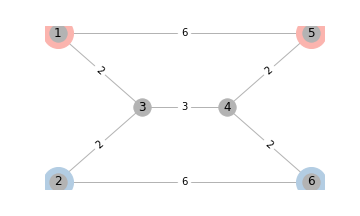
\includegraphics[width=8cm]{../resources/example_1_base.png}
  \caption{Representación de la red utilizada para el ejemplo de aplicación del problema. Los dos pares origen-destino se detallan con un color diferente. Cada arco tiene una etiqueta con el costo de usuario sobre la red de calles.}
  \label{fig:example1base}
\end{figure}

Podemos deducir de la Figura \ref{fig:example1base}, que el camino más corto para ambos pares origen-destino sobre la red de calles está compuesto por un solo arco de costo 6. El objetivo entonces es decidir dónde construir tecnología 1 tal que el costo de los caminos más cortos de uno o ambos pares origen-destino sea menor a 4 unidades (dada la función de transferencia de demanda), de manera que una cantidad $D$ o $2D$ de demanda total pueda ser transferida a la bicicleta. Nótese que los valores posibles de demanda transferida total en este caso solo pueden ser $0$, $D$ y $2D$. Si decidimos utilizar tecnología 1 en alguno de los arcos (1, 5) o (2, 6), digamos el primero, entonces nos aseguramos que la demanda del par origen-destino (1, 5) será transferida a la bicicleta, ya que el costo del camino más corto pasa a ser $3$. Con el presupuesto remanente de valor $5$, solamente podremos construir tecnología 1 en a lo sumo dos de los arcos (2, 3), (3, 4) y (4, 6). No es difícil ver que a lo sumo podremos mejorar el costo del camino más corto a $4.5$ para el par origen-destino (2, 6). La demanda transferida total en este caso es entonces de $D$.

La solución óptima consiste en construir tecnología 1 en todos los arcos del grafo menos los (1, 5) y (2, 6). Esto permite que ambos pares origen-destino tengan un nuevo recorrido como camino más corto, de costo $3.5$, lo que permite, según la función de transferencia de demanda, transferir $2D$ unidades de demanda. Esta solución se puede observar gráficamente en la Figura \ref{fig:example1solution}. El hecho de que los caminos más cortos circulen únicamente por arcos donde hay tecnología 1 es casual y pueden existir, en otras instancias, soluciones óptimas cuyos flujos circulen en parte por la red de calles.

\begin{figure}[h!]
  \centering
  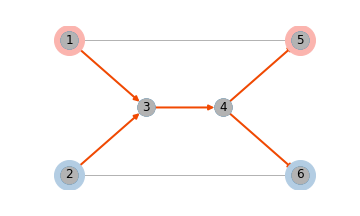
\includegraphics[width=8cm]{../resources/example_1_infras.png}
  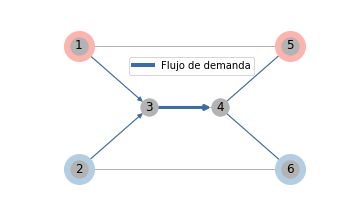
\includegraphics[width=8cm]{../resources/example_1_flows.png}
  \caption{Representación de la solución óptima en el grafo. Arriba se muestra en naranja en cuáles arcos se construye la tecnología 1. Abajo, en azul, los flujos sobre los caminos más cortos para ambos pares origen-destino. Nótese que el ancho del arco en este caso da una noción de la cantidad flujo.}
  \label{fig:example1solution}
\end{figure}

\FloatBarrier
\clearpage
\section{Formulación matemática de dos niveles}

Presentamos la formulación matemática. Sean los siguientes conjuntos, parámetros y variables:

\begin{description}
  \item[$I$]: Conjunto índice de tipos de tecnologías de ciclovías, numeradas desde $0$ en adelante. Se cumple que a mayor valor del índice mejor es la tecnología para el usuario, es decir tiene menor costo de usuario, y mayor el costo de construcción. El índice 0 corresponde a la calle y representa la no construcción de infraestructura de ciclovía.
  \item[$A_n^+$]: Conjunto de arcos que salen del nodo $n \in N$, $A_n^+ \subseteq A$.
  \item[$A_n^-$]: Conjunto de arcos que entran al nodo $n \in N$, $A_n^- \subseteq A$.
  \item[$C_{ai}$]: Parámetro que modela el costo de usuario de atravesar el arco $a \in A$ utilizando la tecnología $i \in I$, $C_{ai} > 0$.
  \item[$H_{ai}$]: Parámetro que modela el costo de construcción de la tecnología $i \in I$ sobre el arco $a \in A$, $H_{ai} \geq 0$.
  \item[$B$]: Parámetro que contiene el valor de presupuesto de construcción de infraestructura de ciclovía, expresado en las mismas unidades de los valores $H_{ai}$.
  \item[$\theta_{nk}$]: Parámetro que vale 1 si $n \in N$ es el origen del par origen-destino $k \in OD$, -1 si es el destino y 0 en otro caso.
  \item[$y_{ai}$]: Variable binaria de primer nivel que determina si la tecnología $i \in I$ está activa, es decir construida, en el arco $a \in A$. La representamos con el vector $y$ en la maximización de primer nivel.
  \item[$x'_{ak}$]: Variable de segundo nivel que determina si el arco $a \in A$ es parte del camino más corto para el par origen-destino $k \in OD$. La representamos con el vector $x'$ en la minimización de segundo nivel.
  \item[$x_{ak}$]: Variable de primer nivel que toma el valor de $x'_{ak}$ en la solución óptima del problema de segundo nivel. La representamos con el vector $x$ en la minimización de primer nivel.
  \item[$w_k$]: Variable de primer nivel que contiene el valor del camino más corto para el par origen-destino $k \in OD$ una vez que se impactan las decisiones dadas por $y_{ai}$. La representamos con el vector $w$ en la maximización de primer nivel.
  \item[$f_k$]: Función que determina la demanda que utiliza la bicicleta como modo de transporte en función del costo del camino más corto para el par origen-destino $k \in OD$.
\end{description}

Definimos la siguiente formulación de programación matemática:

\begin{align}
  \max_{w,x,y}   & \sum_{k \in OD} f_k(w_k)                                                         & \label{eq:objective1lvl} \\
  \text{s.t.}\;  & \sum_{a \in A} \sum_{k \in OD} \sum_{i \in I} C_{ai}y_{ai}x_{ak} = w_k           & \forall k \in OD \label{eq:shortestpath} \\
                 & \sum_{a \in A} \sum_{i \in I} H_{ai}y_{ai} \leq B                                & \label{eq:respectbudget} \\
                 & \sum_{i \in I} y_{ai} = 1                                                        & \forall a \in A \label{eq:alwaysoney} \\
                 & y_{ai} \in \{0,1\}                                                               & \forall a \in A, i \in I \nonumber \\
                 & x \in \argmin_{x'} \sum_{a \in A} \sum_{k \in OD} \sum_{i \in I} C_{ai}y_{ai}x'_{ak}  & \label{eq:subproblem} \\
                 & \qquad \text{s.t.} \sum_{a \in A_n^+} x'_{ak} - \sum_{a \in A_n^-} x'_{ak} = \theta_{nk}   & \forall n \in N, k \in OD \label{eq:flowbalance} \\
                 & \qquad \modelspace x'_{ak} \geq 0                                                          & \forall a \in A, k \in OD \nonumber
\end{align}

Donde:

\begin{description}
  \item[(\ref{eq:objective1lvl})]: Función objetivo de nivel superior, es la suma de los valores de demanda para cada par origen-destino que decidieron usar la bicicleta.
  \item[(\ref{eq:shortestpath})]: Restricción que determina el costo del camino más corto dado en el primer nivel, utilizada para facilitar la lectura del modelo.
  \item[(\ref{eq:respectbudget})]: Restricción de presupuesto sobre las tecnologías de ciclovías que pueden ser construidas.
  \item[(\ref{eq:alwaysoney})]: Restricción que requiere que una y solo una tecnología esté activa en cada arco.
  \item[(\ref{eq:subproblem}) y (\ref{eq:flowbalance})]: Función objetivo del segundo nivel y restricción de balance de flujo. Resuelven el problema del camino más corto para cada par origen-destino modelando el comportamiento de los usuarios.
\end{description}

\section*{Discusión sobre la formulación}

La formulación (\ref{eq:objective1lvl})-(\ref{eq:flowbalance}) denota un problema de programación binivel, o {\it BLPP} de sus siglas en inglés. Los problemas de primer y segundo nivel son llamados también líder y seguidor respectivamente. Estos nombres nos dan una idea de la jerarquía y de la naturaleza de esta formulación. Las variables relevantes del problema líder son las $y_{ak}$ que modelan los tipos de tecnologías construidos en cada arco y una vez que el líder selecciona un valor del vector $y = \left( y_{ak}: a \in A, k \in OD \right)$, estas variables se tornan constantes para el problema seguidor. La naturaleza secuencial de las decisiones implica que las variables de segundo nivel $x'_{ak}$ se pueden ver en función de $y$, es decir, $x' = x'(y)$, aunque en general no se usa esta notación \parencite{bardbook}. Omitimos en esta discusión las variables $w_k$ por ser un agregado de las variables $x_{ak}$ sobre $a \in A$.

Vale le pena mencionar que buscamos resolver en última instancia un problema de optimización lineal para poder acceder a métodos eficientes de resolución y aplicar el modelo a instancias de gran tamaño, como lo son las instancias reales. La formulación planteada en su estado actual no lo es por las ecuaciones (\ref{eq:shortestpath}) y (\ref{eq:subproblem}), y depende de la formulación explícita de las funciones $f_k$, $k \in OD$. Profundizaremos al respecto en el Capítulo \ref{sect:problemresolution}, página \pageref{sect:problemresolution}.

% \subsection{Costos y presupuesto}

Los parámetros más relevantes de la formulación son los que modelan los costos de usuario $C_{ai}$ y costos de construcción $H_{ai}$ para cada par de arcos y tipos de tecnologías de cilcovías. Para el problema de primer nivel, las decisiones sobre cuáles tecnologías construir están limitadas por el costo de construcción total, restricción (\ref{eq:respectbudget}). Las unidades de los costos de construcción por arco y tecnología $H_{ai}$ y presupuesto total $B$ son las mismas y pueden estar expresadas en cualquier unidad monetaria o valor que les de un carácter de bien económico. Por otro lado, los costos de usuario $C_{ai}$ son relevantes para el problema de segundo nivel, ya que es en función de estos que se realiza la optimización. El carácter de estos también es económico, porque dado un bien, por ejemplo trasladarse entre dos puntos de la red, a menor costo mejor; pero su interpretación está orientada a utilidad o beneficio que le brinda al usuario. Hay una relación entre los costos de construcción y los costos de usuario respecto a las tecnologías $I$ y es que a mayor costo de construcción (mejor tecnología) menor es el costo de usuario, considerado por unidad de distancia. Por ejemplo, construir una ciclovía pavimentada exclusiva para los ciclistas es más deseable para estos (y más costoso de construir) que una ciclovía que consiste en una sección de la calle reservada para el tránsito en bicicleta.

% \subsection{Modelado de tecnologías y caminos de los usuarios}

En la formulación del problema de primer nivel, la restricción (\ref{eq:alwaysoney}) pudo haber sido escrita de manera que a lo sumo una tecnología esté activa por arco, es decir, dejar la posibilidad de que no haya infraestructura en un arco. Esto se puede ver de diferentes maneras. Pensando en la realidad modelada, un ciclista podría circular prácticamente por cualquier calle sin problemas, entonces para que las instancias de la formulación (\ref{eq:objective1lvl})-(\ref{eq:flowbalance}) sean semánticamente correctas debería existir una tecnología $i_{base} \in I$ cuyo costo de construcción $H_{ai_{base}}$ sea 0 en todos de los arcos $a \in A$. Utilizamos el índice 0 para dicha tecnología, es decir $i_{base} = 0$. Desde un punto de vista formal, si no se requiere que en cada arco haya siempre una tecnología activa, se complejiza la formulación al representar de dos maneras los costos de usuario: por un lado, el costo de usuario de circular por la calle que es siempre permitido y por otro el costo de circular por una de las tecnologías especializadas si está activa. Por otro lado, si dejamos la posibilidad de que no haya tecnología activa en un arco, deberíamos agregar al problema de segundo nivel una restricción que evite flujos en arcos donde no hay infraestructura activa, es decir: $x_{ak} \leq \sum_{i \in I} y_{ai}, \forall a \in A, k \in OD$. Con esta restricción, el problema de segundo nivel puede no tener solución factible cuando las tecnologías seleccionadas por el primer nivel no induzcan un subgrafo que conecta todos los pares origen-destino, cosa que no es deseable desde el punto de vista de la validez del modelo binivel, ver demostraciones en el Apéndice \ref{sect:apendixbilevelvalidation}, página \pageref{sect:apendixbilevelvalidation}.

Asumiremos de aquí en adelante que las instancias del problema están bien definidas, esto significa que:

\begin{enumerate}
  \item {$G$ es conexo}
  \item {$\forall k \in OD$ existe un camino $S_k \in G$ con costo de construcción cero, es decir $\sum_{a \in S_k} H_{ai_0} = 0$}, donde $i_0$ es el tipo de tecnología de inversión nula.
\end{enumerate}

% \subsection{Modelado de la atracción de demanda}

Son de nuestro particular interés para la formulación los parámetros que representan la demanda y funciones de transferencia de demanda entre modos. Incurrimos en una simplificación que reduce varios modos de transporte (por ejemplo transporte público, taxi o privado) a uno, y consideramos la transferencia desde este modo agregado a la bicicleta. Por lo tanto, las funciones de transferencia de demanda son funciones de $\mathbb{R}^+$ en $\mathbb{R}^+$, cuyos valores del dominio están expresados en unidad del costo de usuario y sus valores del codominio en unidad de demanda que se transfiere de un modo a otro.

El modelo busca determinar la mayor transferencia de demanda entre dos modos de transporte. Para esto, consideramos que sobre la tecnología base la demanda transferida es cero, es decir, que el costo del camino más corto utilizando la bicicleta únicamente sobre la tecnología base no induce transferencia de demanda. Suponemos que partimos de un conjunto de demanda insatisfecha por la tecnología de ciclovías base, pero potencial, si las condiciones mejoran.

En el caso más general, la decisión de utilizar la bicicleta es multifactorial y depende principalmente de tres tipos de factores \parencite{ortuz2011}:

% Modeling Transport, Ortuzar 2011. Pag. 208
\begin{enumerate}
  \item{
      Características del viajante
        \begin{itemize}
          \item{Edad}
          \item{Nivel socio-económico}
          \item{Otros factores como utilización de auto para el trabajo, llevar niños a la escuela, etc.}
        \end{itemize}
  }
  \item{
      Características del viaje
        \begin{itemize}
          \item{Propósito}
          \item{Momento del día}
        \end{itemize}
  }
\item{\label{bicycleusagefactors}
      Características cuantitativas y cualitativas de las facilidades de transporte
      \begin{itemize}
          \item{Disponibilidad de transporte público}
          \item{Infraestructuras de ciclovías}
          \item{Costo del transporte público y combustibles}
          \item{Comodidad y conveniencia}
          \item{Seguridad y protección}
      \end{itemize}
  }
\end{enumerate}

En este trabajo nos concentramos en el punto \ref{bicycleusagefactors}, exclusivamente en los factores que pueden ser favorecidos por la presencia de ciclovías: infraestructura de ciclovías, comodidad y conveniencia, seguridad y protección. Cada tipo de tecnología de ciclovías puede afectar estos factores de distinta manera, pero siempre los modelamos como un único valor para cada arco mediante el parámetro $C_{ai}$. Sobre los otros factores, asumimos que solo consideramos el universo de demanda que es transferible a la bicicleta. Esto nos ahorra considerar aspectos como si el viaje se hace de noche o si el trabajo requiere un vehículo automotor.

El mecanismo de agregar diferentes factores en un único valor es el concepto de utilidad que se utiliza en los modelos probabilísticos de \textcite{ortuz2011, Pacheco2021}. A diferencia de dichos trabajos, en los que se buscan mayores niveles de utilidad, en el nuestro, al modelarlo como un costo, tenemos que menores valores son más deseables.

El modelado de la red de calles y los distintos tipos ciclovías lo realizamos de manera que sobre la red original puedan implantarse infraestructuras de ciclovías que modifican el costo de usuario de atravesar los arcos de la red. Luego configuramos el costo de usuario en cada arco dependiendo de la tecnología activa del arco. El mismo enfoque se utilizó en \parencite{Lin2013, Zhu2019}. Por otro lado, en \parencite{baya2021} el modelado de diferentes tecnologías de ciclovías se implementó como un grafo multicapas donde cada capa replica la red original. La primera capa es la red de calles, la siguiente capa corresponde a la tecnología de tipo 1 y así sucesivamente. Además, cada nodo está conectado con sus nodos réplica en las capas que corresponden a otras tecnologías. Mediante variables de activación permiten que solo una tecnología esté activa en cada arco de lo que representa la red original. Este diseño permite identificar los flujos que cambian de tipo de ciclovía durante un trayecto con el objetivo de penalizar dicho cambio. Notar que este enfoque también es aplicable a nuestro problema. La diferencia entre nuestro modelado y el de \textcite{baya2021} es que el primero modela los diferentes tipos de tecnología a nivel de formulación y el segundo a nivel de los datos.

  \chapter{Resolución del problema}
\label{sect:problemresolution}

Si bien la formulación binivel (\ref{eq:objective1lvl})-(\ref{eq:flowbalance}) expresa de forma natural lo que queremos resolver, en la práctica los BLPP son de difícil resolución. Ya se ha demostrado en \textcite{bardbook} que, incluso el BLPP lineal con variables continuas, es un problema NP-Hard. Además, los métodos existentes para su transformación a formulaciones de un nivel no son directos. En el Apéndice \ref{sec:kkttransform} mencionamos la metodología más común pero con cierto costo analítico y complejidad de resolución adicional, que consiste en sustituir el problema del segundo nivel por las condiciones de optimalidad de Karush-Kuhn-Tucker (KKT). Esta transformación no necesariamente resulta en un modelo eficiente, ya que necesariamente agrega variables binarias para linealizar restricciones no lineales, aún en el caso en el que el modelo binivel original utilice todas sus variables continuas. En \textcite{kara2004} se plantea una formulación binivel cuyo problema de segundo nivel es el mismo que en nuestro trabajo. En ese caso lo resuelven mediante la transformación de KKT con la consecuencia de que además de las variables binarias agregadas por la transformación debieron imponer integralidad en las variables que modelan el flujo dado que se pierde la unimodularidad, propiedad que presentan algunos problemas de optimización de flujos en redes por la cual se pueden obtener valores óptimos enteros en las variables de flujo relajando la restricción de integralidad dichas variables \parencite{shrijver1986}.

En este trabajo tomamos un camino alternativo reescribiendo la formulación binivel como una de un nivel, basándonos en sus características estructurales y en los valores que tienen sentido para sus parámetros. Previo a esta reestructura debemos adaptar la formulación binivel de manera de que todas sus ecuaciones sean lineales.

Como repaso de la complejidad en tiempo de los problemas de optimización lineal de un nivel, tenemos que los problemas lineales con variables continuas pertenecen a la clase P mientras que los problemas lineales enteros mixtos pertenecen a la clase NP \parencite{dimitris1998}. Sabemos que nuestro problema es NP-Hard, por lo tanto, podemos advertir que no encontraremos en este trabajo un método exacto eficiente para su resolución óptima.

\section{Quitando producto de variables}
\label{sect:variableproductremoval}

Proponemos la siguiente formulación del problema de segundo nivel:

\begin{align}
  \min_{h',x'} & \sum_{k \in K} \sum_{a \in A} \sum_{i \in I} C_{ai} h'_{aki}         & \label{eq:subproblemrefeq1} \\
  \text{s.t.}  & \sum_{a \in A_n^+} x'_{ak} - \sum_{a \in A_n^-} x'_{ak} = \theta_{nk} & \forall n \in N, k \in OD \\
               & 0 \leq h'_{aki} \leq y_{ai}                                          & \forall a \in A, k \in OD, i \in I \\
               & \sum_{i \in I} h'_{aki} = x'_{ak}                                     & \forall a \in A, k \in OD \label{eq:subproblemrefeq4}
\end{align}

La formulación (\ref{eq:subproblemrefeq1})-(\ref{eq:subproblemrefeq4}) es equivalente a la formulación del problema de segundo nivel (\ref{eq:subproblem})-(\ref{eq:flowbalance}) ya que desagrega los flujos para cada tecnología, además de para cada par origen-destino y arco, en la nueva variable $h'_{aki}$. Esto es lo que se modela con el producto $y_{ai} x'_{ak}$. Luego, reemplazando en el problema binivel la variable $x_{ak}$ por $h_{aki}$ y la ecuación (\ref{eq:shortestpath}) por

\begin{equation*}
  \sum_{a \in A} \sum_{i \in I} C_{ai} h_{aki} = w_k,\; \forall k \in OD,
\end{equation*}

 entonces el problema es equivalente con la ventaja de que eliminamos el producto $x_{ak}y_{ai}$ en la formulación de primer nivel.

\section{Formulación alternativa de un nivel}
\label{sect:singlelevelformulation}

Proponemos una formulación alternativa de un nivel que puede ser resuelta por un solver MILP convencional y no incurre en el agregado de nuevas variables. Sobre esta formulación haremos pruebas empíricas que muestran su validez respecto a las características de una solución (definidas en \ref{sect:solutioncharacteristics}). Esta formulación resuelve el mismo problema y podemos obtener de ella tanto un valor de demanda transferida como el conjunto de decisiones de cuáles tecnologías construir y dónde.

La idea surge partiendo de la formulación binivel, quitando el subproblema y agregando sus restricciones al problema de primer nivel bajo el argumento de que las funciones $f_k$ deben ser estrictamente decrecientes para que el problema tenga sentido semánticamente, ya que a mayor costo de usuario menor debería ser la demanda transferida. Entonces para maximizar el objetivo de nuestro problema, $\sum_{j \in OD}f_k(w_k)$, necesitamos que los valores de los costos de los caminos más cortos $w_k, k \in OD$, sean lo más chico posible y, por lo tanto, logramos minimizar también el costo de usuario.

La formulación resultante es la siguiente:

\begin{align}
  \max_{h,w,x,y}          & \sum_{k \in OD} f_k(w_k)                                    & \label{eq:objectivealt} \\
  \text{s.t.}\; & \sum_{a \in A} \sum_{i \in I} C_{ai}h_{aki} = w_k           & \forall k \in OD \label{eq:shortestpathalt} \\
                & \sum_{a \in A} \sum_{i \in I} H_{ai}y_{ai} \leq B           & \label{eq:respectbudgetalt} \\
                & \sum_{i \in I} y_{ai} = 1                                   & \forall a \in A \label{eq:alwaysoneyalt} \\
                & \sum_{i \in I} h_{aki} = x_{ak}                             & \forall a \in A, k \in OD \\
                & h_{aki} \leq y_{ai}                                         & \forall a \in A, k \in OD, i \in I \\
                & \sum_{a \in A_n^+} x_{ak} - \sum_{a \in A_n^-} x_{ak} = \theta_{nk}   & \forall n \in N, k \in OD \label{eq:flowbalancealt} \\
                & x_{ak} \geq 0, h_{aki} \geq 0, y_{ai} \in \{0,1\}                     & \nonumber
\end{align}

Es importante notar que si las funciones son decrecientes (no estrictamente), entonces puede haber valores de costos de caminos más cortos que no tienen incentivo a decrecer si no se logra mayor transferencia de demanda. Esto puede tener implicancias respecto a la ciclovía que se decida construir pero no sobre el valor objetivo del problema. Realizaremos una discusión más profunda al respecto en la sección \ref{sect:formulationanalysis}.

\section{Modelado de transferencia de demanda}
\label{sect:transferfunctiondefs}

Lo que resta definir es cómo modelamos las funciones $f_k$. Nuestro objetivo es definir un mecanismo para que cualquier tipo de función pueda ser expresada como un problema de optimización lineal y que este se pueda acoplar a la formulación existente.

Podemos encontrar en la literatura soluciones al problema de transferencia de demanda. En \textcite{laporte2007} y \textcite{marin2007} se modela la demanda transferida al transporte público de trenes desde el transporte privado. Consideran un parámetro $c^{PRIV}_k,\; k \in OD$ que modela el costo del transporte privado para un par origen-destino $k$. Luego, si la red de transporte público logra un costo menor, entonces se considera que toda la demanda del par origen-destino $k$ se transfiere a dicho modo, lo que se conoce como {\it all-or-nothing}. Utilizando nuestra notación, la demanda transferida para el par origen-destino $k$ en este esquema sería:

\begin{equation}
  \label{eq:allornothing}
  f_k(w_k) = \left\{ \begin{array}{lcr}
    d_k & \mbox{si}   & w_k < C^{PRIV}_k \\
          0 & \mbox{si no} &
  \end{array}
  \right.
\end{equation}

\subsection{Definición propuesta}

Consideramos que una función $f_k$ arbitraria debe poder modelar una transición gradual de la demanda entre modos de transporte cuya curva puede comportarse de diferentes formas como analizamos en el Capítulo \ref{sect:problemresults}. Asumiendo que las funciones $f_k$ son decrecientes, el enfoque que seguimos es representar cada una como una sucesión decreciente de puntos de quiebre, tal que para cada punto exista un valor asociado de cantidad de demanda transferida. Su representación gráfica es una función escalonada donde cada escalón es constante, ver Figura \ref{fig:fdrawexample}. Al momento de evaluar una función representada de esta manera, los puntos de quiebre son comparados contra el valor del camino más corto $w_k$ seleccionando el mínimo punto de valor mayor a $w_k$. Entonces, sea $w_k$ fijo, la demanda transferida para el par origen-destino $k$ es:

\begin{equation}
  \label{eq:deffks}
  f_k(w_k) = P_{j^*},\; j^* = \argmin_{j \in J} \{Q_j \geq w_k\},
\end{equation}

donde $Q_j$ son los puntos de quiebre en la unidad del costo del camino más corto, $J$ es un conjunto índice y $P_{j^*}$ es la cantidad de demanda que se transfiere.

Una ventaja de esta formulación es que puede ser integrada a la función objetivo de la formulación de nuestro problema (\ref{eq:objectivealt})-(\ref{eq:flowbalancealt}), de manera que la minimización queda en manos del objetivo del mismo problema.

Para modelar la función {\it argmin} en una formulación lineal como la que venimos trabajando es necesario utilizar variables de activación que permitan que sólo un valor del conjunto índice esté activo (para cada par origen-destino). Por ejemplo, si se usa $z_j,\; j \in J$, lo antedicho equivale a decir que $z_j \in \{0,1\}$ y $\sum_{j \in J} z_j = 1$. Luego queda en manos de la minimización elegir el $z_j$ activo óptimo.

Nótese que esta definición es una extensión de la {\it all-or-nothing} en (\ref{eq:allornothing}). Para modelarla basta considerar $J = \{0, 1\}$, $P_0 = 0, P_1 = d_k$ y $Q_0 = M, Q_1 = C^{PRIV}_k$, donde $M$ es un número arbitrario grande, mayor a $C^{PRIV}_k$ y $d_k$ es la demanda para el par origen-destino $k$.

\begin{figure}[h!]
  \centering
  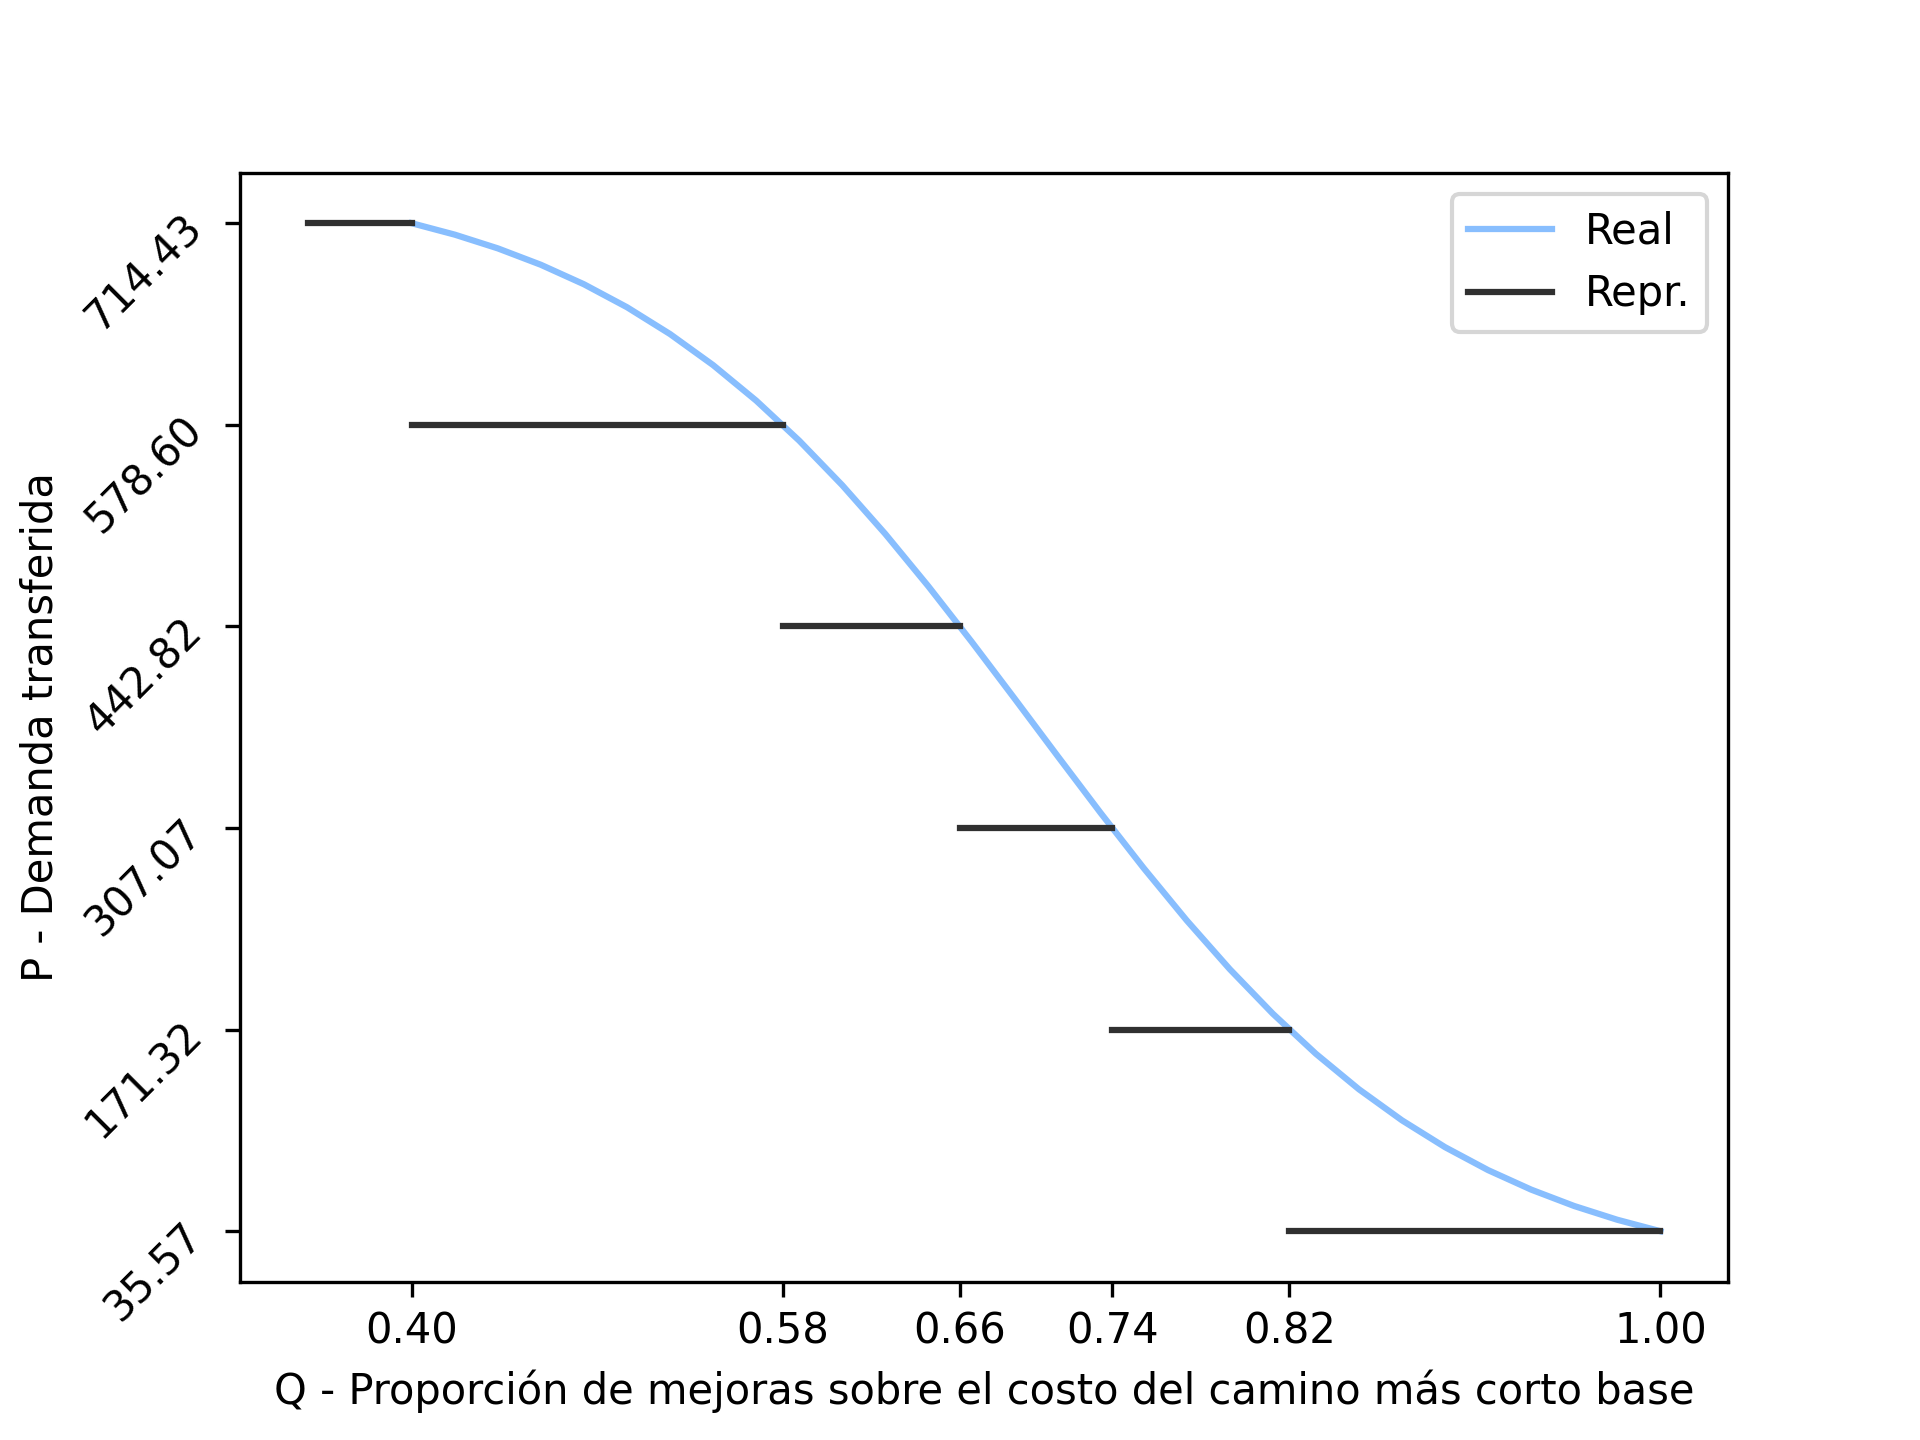
\includegraphics[width=10cm]{../resources/f_example.png}
  \caption{Ejemplo de una función arbitraria y su representación con el mecanismo planteado sobre una demanda total de 750 unidades y un costo del camino más corto base de 1000. Los puntos donde hacer los quiebres son arbitrarios.}
  \label{fig:fdrawexample}
\end{figure}

Una alternativa más precisa de esta representación es la definida en \textcite{crainic2021ch8} donde se presenta un marco para modelar funciones arbitrarias como funciones lineales de a partes con valores de pendiente no nulos entre puntos de quiebre. Esta representación es una generalización de la presentada en nuestro trabajo y permite representar de manera más precisa la función real al costo de mayor complejidad al momento de modelarla como problema de programación lineal. Según los autores, debido a la cantidad de variables y restricciones que se agregan con este método, es recomendable utilizar algoritmos especializados como la descomposición Dantzig-Wolfe.

\subsection{Formulación como problema de programación lineal}

La forma más simple de modelar $f_k$ (o simplemente $f$) es la denotada por (\ref{eq:fkv1eq1})-(\ref{eq:fkv1eq4}). Sea $W \in \mathbb{R}^+$ un valor fijo:

\begin{align}
  f(W) =\; & \max \sum_{j \in J} P_j y_j    & \label{eq:fkv1eq1} \\
           & s.t. \sum_{j \in J} y_j = 1   & \label{eq:fkv1eq2} \\
           & \;\;\; Q_j \geq W y_j         & \label{eq:fkv1eq3} \forall j \in J \\
           & \;\;\; y_j \in \{0,1\}        & \label{eq:fkv1eq4} \forall j \in J
\end{align}

El valor óptimo de esta formulación es el máximo valor $P_j \;|\; Q_j \geq W, j \in J$. La restricción (\ref{eq:fkv1eq3}) deja afuera los valores de $j \in J$ que no cumplen $Q_j \geq W$. Luego, como un único valor de $y_j$ puede estar activo se selecciona aquel que induce el valor máximo de $P_j$ dado que este último está en el objetivo. Sin embargo, esta formulación no puede ser integrada en su presente forma a la formulación (\ref{eq:objectivealt})-(\ref{eq:flowbalancealt}) sin perder linealidad dado que en la última $W$ es modelado con una variable ($w_k$), entonces el resultado sería un problema no lineal por la restricción (\ref{eq:fkv1eq3}). Por este motivo estudiamos dos formulaciones alternativas que logran solucionar esta situación. La idea en ambas es desagregar $W$ como la suma de nuevas variables y utilizar estas en la restricción (\ref{eq:fkv1eq3}) en lugar del producto $W y_j$.

\clearpage
\paragraph*{$f_k$ como problema lineal versión 1}

\begin{align}
  f(W) =\; & \max \sum_{j \in J} P_j y_j             & \label{eq:fkv3eq1}\\
           & s.t. \sum_{j \in J} y_j = 1            & \label{eq:fkv3eq2}\\
           & \;\;\; Q_j \geq w^{aux}_j              & \forall j \in J \label{eq:fkv3eq3} \\
           & \;\;\; w^{aux}_j \leq M y_j            & \forall j \in J \label{eq:fkv3eq4} \\
           & \;\;\; w^{sink}_j \leq M (1 - y_j)     & \forall j \in J \label{eq:fkv3eq5} \\
           & \;\;\; w^{sink}_j + w^{aux}_j = W      & \label{eq:fkv3eq6} \forall j \in J\\
           & \;\;\; y_j \in \{0,1\}                 & \label{eq:fkv3domainy} \forall j \in J \\
           & \;\;\; w^{aux}_j, w^{sink}_j \geq 0    & \label{eq:fkv3eq7} \forall j \in J
\end{align}

Se desagrega $W$ para cada $j$ en $w^{sink}_j + w^{aux}_j$ de manera que uno de los dos tenga el valor de $W$, esto se logra con las restricciones (\ref{eq:fkv3eq4}), (\ref{eq:fkv3eq5}) y (\ref{eq:fkv3eq6}). Entonces, mediante la restricción (\ref{eq:fkv3eq2}), se cumple que únicamente el $w^{aux}_j$ cuyo $y_j$ esté activo tendrá el valor de $W$, mientras que para el resto de los $j$ las variables $w^{sink}_j$ habrán tomado dicho valor. Las mencionadas restricciones sirven para activar $y_i$ y utilizan un parámetro $M \geq W$ arbitrario Las variables $w^{sink}_j$ sirven para absorber el valor de $W$ cuando $y_j$ está inactiva, de manera que se pueda cumplir la restricción (\ref{eq:fkv3eq3}) cuando $W$ es mayor a $Q_j$.

\paragraph*{$f_k$ como problema lineal versión 2}

\begin{align}
  f(W) =\; & \max \sum_{j \in J} P_j y_j             & \label{eq:fkv2eq1}\\
           & s.t. \sum_{j \in J} y_j = 1            & \label{eq:fkv2eq2}\\
           & \;\;\; Q_j \geq w^{aux}_j              & \forall j \in J \label{eq:implfkoriginalineq} \\
           & \;\;\; w^{aux}_j \leq M y_j            & \forall j \in J \label{eq:yactivation1} \\
           & \;\;\; \sum_{j \in J} w^{aux}_j = W    & \label{eq:activatewaux} \\
           & \;\;\; y_j \in \{0,1\}                 & \label{eq:fkv2domainy} \forall j \in J\\
           & \;\;\; w^{aux}_j \geq 0                & \label{eq:fkv2eq6} \forall j \in J
\end{align}

\clearpage
En este caso se desagrega $W$ como suma de $|J|$ variables $w^{aux}_j$ de manera que solo una de ellas esté activa y tenga el valor de $W$. Para activar $y_j$ se agrega la restricción (\ref{eq:yactivation1}) utilizando, igual que en la formulación anterior, un parámetro $M \geq W$. Finalmente, las restricciones (\ref{eq:fkv2eq2}) y (\ref{eq:activatewaux}) logran que solo uno de los $w^{aux}_j$ tome el valor de $W$ y el resto sean 0.

\subsection{Discusión de las formulaciones de transferencia de demanda}

Según definimos $f_k(W)$ en (\ref{eq:deffks}), sea $p = f_k(W)$, entonces se debe cumplir que:

\begin{enumerate}[(a)]
  \item {\label{deffpt1} $p$ es exactamente uno de los valores del conjunto de valores $P_j$, es decir: $p \in \{P_j\}_{j \in J}$}
  \item {\label{deffpt2} Sea $\hat{j} = j \;|\; p = P_j$. Se cumple que el valor $Q$ del punto de quiebre asociado a $\hat{j}$ no es menor que el costo del camino más corto $W$, es decir: $Q_{\hat{j}} \geq W$.}
  \item {\label{deffpt3} Dado el $\hat{j}$ anterior, entonces no existe un punto de quiebre $Q_j \; \forall j \in J\setminus\{\hat{j}\}$ que sea no mayor al punto de quiebre $Q_{\hat{j}}$ y mayor o igual al costo del camino más corto, es decir: $\not{\exists}\; Q_j\; \forall j \in J\setminus\{\hat{j}\} \;|\; Q_j \in  [W, Q_{\hat{j}}]$}.
\end{enumerate}

Es de nuestro interés analizar la correctitud de las formulaciones respecto a las propiedades mencionados. Para la versión 1, tenemos que la propiedad \ref{deffpt1} se cumple en la función objetivo donde se establece el valor objetivo como la suma sobre el conjunto $\{P_j\}_{j \in J}$, además la restricción (\ref{eq:fkv3eq2}) establece que solo uno de esos valores puede estar activo en la suma del objetivo dado el dominio de la variable $y_j$. Luego, la propiedad \ref{deffpt2} se cumple dado que $y_{\hat{j}} = 1$ por la propiedad anterior, entonces $w_{\hat{j}}^{aux} = W$ por restricciones (\ref{eq:fkv3eq4}), (\ref{eq:fkv3eq5}) y (\ref{eq:fkv3eq6}) y la restricción (\ref{eq:fkv3eq3}) verifica la propiedad en cuestión. Finalmente, la propiedad \ref{deffpt3} se cumple por el hecho de que la función objetivo es una maximización y que $f(W)$ es una función estrictamente decreciente, entonces, si existiera un $Q_a \in \{Q_j\}_{j \in J} \;|\; Q_a < Q_{\hat{j}} \;\text{y}\; Q_a \geq W, a \in J$, existe un valor $P_a > P_{\hat{j}}$, lo que contradice el hecho de que el objetivo sea una maximización.

Podemos utilizar las mismas justificaciones de las propiedades \ref{deffpt1} y \ref{deffpt3} para la versión 2 de la formulación. Luego, la propiedad \ref{deffpt2} se cumple dado que $y_{\hat{j}} = 1$ por las propiedades anteriores y considerando que $w^{aux}_{\hat{j}} = W$ por las restricciones (\ref{eq:fkv2eq2}), (\ref{eq:yactivation1}) y (\ref{eq:activatewaux}) tenemos que la condición se cumple en la restricción (\ref{eq:implfkoriginalineq}).

\subsection{Valores posibles de $P_j$ y $Q_j$}

Los valores que pueden ser utilizados para los conjuntos $Q$ y $P$ son cualquier subconjunto discreto del dominio de la función de transferencia de demanda y su valor funcional, respectivamente. Dada una instancia del problema y un par origen destino $k$, llamamos $\underline{W}$ al costo del camino más corto suponiendo que las mejores tecnologías se pueden construir y $\overline{W}$ al costo del camino más corto sobre el grafo base (sin infraestructura de ciclovía especializada)\footnote{En realidad, $\overline{W}$ es el mínimo valor para el que $f_k$ es mínimo, podría ser cualquier número arbitrariamente grande.}. Entonces $Q_j \in [\underline{W}, \overline{W}],\; \forall j \in J$. Los valores de $Pj$ son la cantidad de demanda que se transfiere para cada $Q_j$, es decir $P = \{f_k(Q_j):\; j \in J\}$. El conjunto índice $J$ determina la precisión con que se representa la función $f_k$ y el orden en que define los puntos de quiebre es el siguiente: sea $J = \{1, 2, .. , J_{max}\}$, entonces $P_j < P_{j+1}$ y $Q_j > Q_{j+1}$, es decir, a mayor valor del índice $j$ mayor es el valor de demanda transferida y mejor es el camino para el usuario.

Además, entendemos que tiene sentido que el dominio de $f_k$ sean valores de costos de usuario de camino más cortos que van desde aquel para el cual toda la demanda se transfiere hasta aquel para el cual no hay demanda transferida. Es decir, que el mínimo de $f_k$ sea 0 y que el máximo sea la demanda total del par $k$ ($d_k$), esto es $f_k(\overline{W}) = 0$ y $f_k(\underline{W}) = d_k$. Esto quiere decir que si no hay infraestructura de ciclovías o la infraestructura construida no afecta el costo del camino más corto entonces no debe haber transferencia de demanda. Por otro lado, si la mejor tecnología posible es construida de manera que el costo del camino más corto disminuya a $\underline{W}$ entonces toda la demanda se transfiere. Lo anterior es consistente con la hipótesis de que trabajamos exclusivamente con la demanda transferible a la bicicleta dejando afuera la que ya utiliza dicho medio de transporte, la que en ningún caso la utilizaría y la que requiere de costos de usuario demasiado bajos en comparación con lo que puede ofrecer la mejor tecnología de ciclovía. Por lo tanto, en la definición de una función $f_k, k \in OD$, tienen relevancia aspectos como el grafo base y el costo del camino más corto sobre él para el par origen-destino $k$ y las tecnologías de ciclovías que pueden ser construidas y cómo afectan al costo de usuario al ser activadas.

Una forma posible de establecer los valores de $J$, $P_j$ y $Q_J$ es: dada una función $f_k$, tomando $N$ valores equidistantes entre $[\underline{W}, \overline{W}]$ obtendremos $Q_j$ y tomando el valor funcional de esos puntos obtendremos $P_j$, luego $J=\{1,..,N\}$.

\section{Formulación integrada}
\label{sect:alltogether}

Luego del análisis hecho en las secciones \ref{sect:variableproductremoval}, \ref{sect:singlelevelformulation} y \ref{sect:transferfunctiondefs}, ensamblamos la formulación MILP de un nivel de manera explícita. Dado que tenemos dos variantes del modelado de las funciones de transferencia de demanda entonces también tendremos dos variantes de esta formulación. Aquí presentamos la formulación completa utilizando la versión 2 del modelado de las funciones de transferencia, siendo la otra muy similar. Fundamentalmente sobre estas dos variantes trabajamos en lo que sigue.

Además de las definiciones en la formulación inicial (\ref{eq:objective1lvl})-(\ref{eq:flowbalance}), agregamos las siguientes, algunas de las cuales ya las mencionamos, pero las incluimos para facilitar la lectura:

\begin{description}
  \item[$J$]: Conjunto índice utilizado en los conjuntos $P$ y $Q$.
  \item[$P_{kj}$]: Parámetro que determina la cantidad de demanda transferida para el par origen-destino $k \in OD$ y el índice $j \in J$.
  \item[$Q_{kj}$]: Parámetro que contiene el punto de quiebre para determinar la demanda transferida para el par origen-destino $k \in OD$ e índice $j \in J$.
  \item[$M$]: Número positivo muy grande.
  \item[$z_{kj}$]: Variable binaria que determina si la demanda transferida para el par origen-destino $k \in OD$ es la de índice $j \in J$.
  \item[$h_{aki}$]: Variable no negativa que determina el flujo que pasa por el arco $a \in A$, para el par origen-destino $k \in OD$ utilizando la tecnología $i \in I$.
  \item[$w^{aux}_{kj}$]: Variable no negativa que contiene el valor de $w_{k}$ si $z_{kj}$ está activa y de lo contrario cero.
\end{description}

La formulación que resulta de la integración de (\ref{eq:objectivealt})-(\ref{eq:flowbalancealt}) que define la formulación de un nivel, de (\ref{eq:subproblemrefeq1})-(\ref{eq:subproblemrefeq4}) que quita el producto de variables y de (\ref{eq:fkv2eq1})-(\ref{eq:fkv2eq6}) que define la versión 2 de las funciones de transferencia de demanda es la siguiente:

\begin{align}
  \max_{h,k,x,y,w,z} & \sum_{k \in OD} \sum_{j \in J} P_{kj} z_{kj}                          & \label{eq:objectivefinalalt} \\
  \text{s.t.}\; & \sum_{a \in A} \sum_{i \in I} C_{ai}h_{aki} = w_k                     & \forall k \in OD \label{eq:shortestpathaltfinal} \\
                & Q_{kj} \geq w^{aux}_{kj}                                              & \forall j \in J, k \in OD \label{eq:breakpointsalt} \\
                & w^{aux}_{kj} \leq M z_{kj}                                            & \forall j \in J, k \in OD \\
                & \sum_{j \in J} w^{aux}_{kj} = w_k                                     & \forall k \in OD \\
                & \sum_{j \in J} z_{kj} = 1                                             & \forall k \in OD \label{eq:singularbreakpointalt} \\
                & \sum_{a \in A} \sum_{i \in I} H_{ai}y_{ai} \leq B                     & \label{eq:respectbudgetaltfinal} \\
                & \sum_{i \in I} y_{ai} = 1                                             & \forall a \in A \label{eq:alwaysoneyaltfinal} \\
                & \sum_{a \in A_n^+} x_{ak} - \sum_{a \in A_n^-} x_{ak} = \theta_{nk}   & \forall n \in N, k \in OD \label{eq:flowbalancealtfinal} \\
                & \sum_{i \in I} h_{aki} = x_{ak}                                       & \forall a \in A, k \in OD \label{eq:flowactivationalt} \\
                & h_{aki} \leq y_{ai}                                                   & \forall a \in A, k \in OD, i \in I \label{eq:respectinfraalt} \\
                & z_{kj} \in \{0,1\}                                                    & \forall k \in OD, j \in J \nonumber \\
                & y_{ai} \in \{0,1\}                                                    & \forall a \in A, i \in I \nonumber \\
                & h_{aki} \geq 0                                                        & \forall a \in A, k \in OD, i \in I \nonumber
\end{align}

Donde las nuevas ecuaciones son:

\begin{description}
  \item[\ref{eq:objectivefinalalt}]: Función que suma los valores de demanda transferida $P_{kj}$ correspondiente a los puntos de quiebre activos.
  \item[\ref{eq:breakpointsalt}]: Restricción que determina que los puntos de quiebre activos, son aquellos cuyo costo es menor o igual al del camino más corto.
  \item[\ref{eq:singularbreakpointalt}]: Restricción que permite solo un punto de quiebre activo para cada par origen-destino $k \in OD$.
  \item[\ref{eq:flowactivationalt}]: Restricción que fija el valor del flujo por arco por par origen-destino en base al flujo por arco, par origen-destino y tecnología.
  \item[\ref{eq:respectinfraalt}]: Restricción que limita el flujo desagregado por arco y tecnología ($h_{aki}$) a la tecnología activa en el arco. El flujo por el arco $a \in A$, para el par origen-destino $k \in OD$ y la tecnología $i \in I$ puede estar activo si la tecnología $i$ está activa.
\end{description}

\section{Análisis de la formulación propuesta}
\label{sect:formulationanalysis}

En esta sección analizamos las dos variantes de la formulación de un nivel (\ref{eq:objectivefinalalt})-(\ref{eq:respectinfraalt}) con pequeñas variantes adicionales y mostramos su validez de manera experimental.

Como mecanismo de validación, utilizamos las características que debe cumplir una solución, mencionadas al principio en la sección \ref{sect:solutioncharacteristics}, página \pageref{sect:solutioncharacteristics}. Comprobando dichas condiciones sobre las soluciones obtenidas por las formulaciones estudiadas podemos tener confianza de que ellas resuelven el problema especificado originalmente. Este proceso también fue de utilidad verificar la implementación computacional durante su desarrollo.

% \subsection{Variantes de la formulación}

Durante la implementación y pruebas preliminares de la formulación (\ref{eq:objectivefinalalt})-(\ref{eq:respectinfraalt}) observamos que en algunos casos los flujos no eran consistentes con la hipótesis del comportamiento de los usuarios, es decir, no iban por el camino más corto entre origen y destino. La explicación es que las funciones $f_k$ son constantes entre dos valores consecutivos de $Q_{kj}$ lo cual causa que en dicho dominio no exista incentivo para optimizar el costo del camino más corto. Para corregir esto consideramos dos opciones, que en definitiva cambian nuestra formulación de un objetivo único a una multiobjetivo donde el objetivo primario sigue siendo el de maximizar la demanda transferida total (\ref{eq:objectivefinalalt}) y el secundario se presenta a continuación en dos variantes.

En la primera opción agregamos variables de holgura $r_{kj} \geq 0$ que modelan la diferencia entre el punto de quiebre $Q_{kj}$ activo y el costo del camino más corto para un par origen-destino $k$, es decir $w^{aux}_{kj}$. Dichas variables también son agregadas a la función objetivo como objetivo adicional lo que incentiva a las variables $w^{aux}_{kj}$ a decrecer en favor del aumento de $r_{kj}$. Esto cambia el modelado de las funciones $f_k$ en la ecuación (\ref{eq:breakpointsalt}) que queda de la siguiente manera:

\begin{equation}
  \label{eq:multipleobj1breakpoint}
  Q_{kj} z_{kj} - r_{kj} = w^{aux}_{kj}
\end{equation}

Vale la pena notar que esta restricción se encuentra en ambas versiones de las formulaciones de las funciones de transferencia de demanda, por lo tanto, en ambos casos se aplica esta variante.

Luego, sea el parámetro $\beta \geq 0$, entonces la función multiobjetivo 1 es la siguiente:

\begin{equation}
  \label{eq:multipleobj1}
  \sum_{k \in OD} \sum_{j \in J} \left( P_{kj}z_{kj} + \beta r_{kj} \right)
\end{equation}

Otra forma de abordar esta situación es vincular los objetivos de los problemas de primer y segundo nivel en (\ref{eq:objective1lvl})-(\ref{eq:flowbalance}). Dado que los dos objetivos optimizan en direcciones contrarias entonces el coeficiente del objetivo añadido, que originalmente era una minimización, necesita ser un valor negativo. Sea el parámetro $\rho \geq 0$, entonces podemos expresar la función multiobjetivo 2 como:

\begin{equation}
  \label{eq:multipleobj2}
  \sum_{k \in OD} \left[ -\rho w_k + \sum_{j \in J} P_{jk}z_{kj} \right]
\end{equation}

Notar que al modificar el objetivo del problema estamos, estrictamente hablando, solucionando otro problema. Sin embargo, a los efectos prácticos podemos en este caso encontrar valores de los pesos relativos de cada objetivo añadido de manera de que las versiones multiobjetivo resuelvan correctamente nuestro problema en términos de demanda transferida óptima y se pueda calcular la demanda transferida total con posterioridad a la resolución. Dicho de otra manera, para cada peso $\beta$ y $\rho$ existe un intervalo $[0, \beta_{max}]$ y $[0, \rho_{max}]$ respectivamente, en el que el valor computado de demanda transferida es la misma e igual al valor objetivo de la formulación de un único objetivo (\ref{eq:objectivefinalalt})-(\ref{eq:respectinfraalt}). Tenemos diferentes interpretaciones para cada objetivo auxiliar. En el caso de la formulación multiobjetivo 1, dado que ambos objetivos tienen el mismo signo, lo que tiene que suceder, intuitivamente, es que el valor del objetivo auxiliar sea intrascendente respecto a los saltos posibles en los puntos de quiebre para cada par origen destino, lo que permite que ambos objetivos puedan comportarse de manera independiente. En el caso de la formulación multiobjetivo 2, dado que los objetivos tienen signos opuestos, no hay límites en el valor máximo de $\rho$, por lo que diremos que $\rho_{max} > 0$.

Las soluciones obtenidas por las versiones multiobjetivo son potencialmente mejores, respecto a la ciclovía resultante, en comparación al modelo binivel en términos de la red de ciclovía resultante. Esto se debe a que estamos adicionando un objetivo secundario para obtener valores óptimos de los caminos y al ser éste parte del objetivo del MILP el modelo intentará obtener una asignación de tecnologías activas que minimicen este valor. Por el otro lado, la formulación binivel no necesariamente busca esto, ya que el único objetivo es maximizar la demanda transferida mientras que los flujos óptimos son solo información que permite llegar al objetivo. Podemos utilizar la transformación de KKT del Apéndice \ref{sec:kkttransform} para visualizar esto: esta transformación sustituye el subproblema por un sistema de ecuaciones que se agregan como restricción al problema de primer nivel, entonces el problema transformado busca maximizar la demanda transferida total sobre un espacio de soluciones factibles compuesto por las variables $(y, x)$ donde $y$ es la asignación de infraestructuras que no exceden el presupuesto y $x$ son los flujos que inducen caminos óptimos. Si hay dos valores $(y_1, x_1)$ e $(y_2, x_2)$ que inducen la misma cantidad de demanda transferida, no hay ninguna condición en esta última transformación que permita decidir una sobre la otra mientras que en las multiobjetivo se elegirá aquella con caminos más cortos.

\subsection{Ejemplo - Comparativa de variantes de un objetivo y multiobjetivo}
\label{sect:example2}

Este ejemplo busca ilustrar por qué es necesario agregar nuevos objetivos a la función objetivo de formulación (\ref{eq:objectivefinalalt})-(\ref{eq:respectinfraalt}) de forma de optimizar no solo la demanda transferida, sino que también obtener una buena decisión de ubicación y tipo de tecnología de ciclovías.

Para este ejemplo utilizaremos como base la red descrita en la Tabla \ref{table:example2arccosts} y en la Figura \ref{fig:example2base}. Consideramos dos tipos de tecnologías, la base o red de calles y la tecnología 1, que reduce el costo de usuario de la primera a la mitad; un par origen-destino, $(1, 6)$ con demanda $D$, un presupuesto de 5 y la siguiente función de transferencia de demanda:

$$
  f(x) = \left\{ \begin{array}{lcr}
          D & \mbox{si}   & x \leq 4.5 \\
          0 & \mbox{si no} &
        \end{array}
        \right.
$$

\begin{table}[h!]
  \centering
  \begin{tabular}{ccScc}
    \toprule
      Arco & CU base & {CU 1} & CC base & CC 1 \\
    \midrule
      (1, 2) & 3 & 1,5 & 0 & 3 \\
      (1, 3) & 3 & 1,5 & 0 & 3 \\
      (1, 5) & 4 & 2   & 0 & 4 \\
      (2, 3) & 2 & 1   & 0 & 2 \\
      (2, 4) & 3 & 1,5 & 0 & 3 \\
      (3, 2) & 3 & 1,5 & 0 & 3 \\
      (3, 4) & 2 & 1   & 0 & 2 \\
      (3, 5) & 2 & 1   & 0 & 2 \\
      (4, 5) & 4 & 2   & 0 & 4 \\
      (4, 6) & 2 & 1   & 0 & 2 \\
      (5, 4) & 4 & 2   & 0 & 4 \\
      (5, 6) & 2 & 1   & 0 & 2 \\
    \bottomrule
  \end{tabular}
    \caption{Costos de usuario (CU) y de construcción (CC) para cada tecnología de ciclovía.}\label{table:example2arccosts}
\end{table}

\begin{figure}[h!]
  \centering
  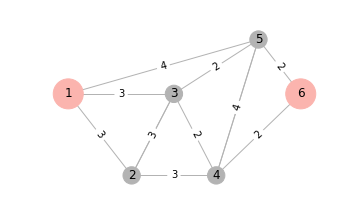
\includegraphics[width=8cm]{../resources/example_2_base.png}
  \caption{Red utilizada para el ejemplo de beneficio de variantes multiobjetivo. Los arcos están ponderados por el costo de usuario de la red de calles que coincide con el costo de construcción de la tecnología 1. El camino más corto sobre el grafo base es el (1, 5), (5, 6) de costo 6.}
  \label{fig:example2base}
\end{figure}

\FloatBarrier

Presentamos dos soluciones: la S utilizando la variante de un único objetivo (\ref{eq:objectivefinalalt})-(\ref{eq:respectinfraalt}) y la SM utilizando cualquiera de las variantes multiobjetivo (ecuaciones (\ref{eq:multipleobj1}) o (\ref{eq:multipleobj2})).

La solución S, representada en la Figura \ref{fig:example2solv2}, tiene las siguientes características:

\begin{itemize}
  \item{Demanda transferida total: $D$}
  \item{Tecnología de tipo 1 construida en arcos (1, 3) y (4, 6)}
  \item{Presupuesto utilizado: 5}
  \item{El camino más corto es (1, 3), (3, 4), (4, 6) con costo 4,5}
\end{itemize}

Mientras que la solución SM, en la Figura \ref{fig:example2solv1}, tiene las siguientes características:

\begin{itemize}
  \item{Demanda transferida total: $D$}
  \item{Tecnología de tipo 1 construida en el arco (1, 5)}
  \item{Presupuesto utilizado: 4}
  \item{El camino más corto es (1, 5), (5, 6) con costo 4}
\end{itemize}

Observamos que la solución SM es mejor en términos de la infraestructura de ciclovía a construir que la de un único objetivo, ya que el costo de usuario resultante disminuyó en mayor cantidad y el presupuesto utilizado fue menor, aunque esto último es circunstancial. Para analizar la causa, primero debemos definir los puntos de quiebre de esta instancia. Dada la simplicidad de la función de transferencia de demanda podemos utilizar solo dos puntos de quiebre, entonces $J = \{0, 1\}$, $Q = \{6, 4.5\}$ y $P = \{0, D\}$. Omitiremos los índices $k$ del par origen-destino dado que existe uno solo. Tenemos que el $z_j$ activo, que determina el valor de demanda transferida, es aquel con $j = 1$ dado que sabemos que la demanda transferida es $D$.

Considerando la opción multiobjetivo 1 (\ref{eq:multipleobj1}), tenemos de la restricción (\ref{eq:multipleobj1breakpoint}) que $r_1 = Q_1 - w^{aux}$, y siendo $w^{aux} = w$ por ser el punto de quiebre activo, entonces $r_1 = 4.5 - w$ y el valor objetivo es $D + r_1$. Aplicando las soluciones a estas ecuaciones tenemos que para la solución S se cumple que $r_1 = 0$ y para SM se cumple que $r_1 = 0.5$. Por lo tanto, la presencia de $r_{kj}$ en el objetivo ayuda a elegir la solución SM sobre la S en este caso.

Si utilizamos la formulación multiobjetivo 2 (\ref{eq:multipleobj2}), tenemos que el valor objetivo evaluado en la solución S es $D - 4.5$ y en la solución SM es de $D - 4$, por lo tanto, la solución SM también es mejor según esta formulación.

Vale la pena aclarar que la solución SM es, para la versión de un único objetivo, tan buena como la S. En general, asumiendo que los pesos $\beta$ y $\rho$ fueron elegidos de acuerdo a la sección anterior (\ref{sect:formulationanalysis}), las soluciones obtenidas por las versiones multiobjetivo también son soluciones óptimas de la de un único objetivo.

Finalizamos este ejemplo comentando que ambas soluciones S y SM satisfacen las condiciones o características de una solución definidas en la sección (\ref{sect:solutioncharacteristics}), página \pageref{sect:solutioncharacteristics}.

\begin{figure}[h!]
  \centering
  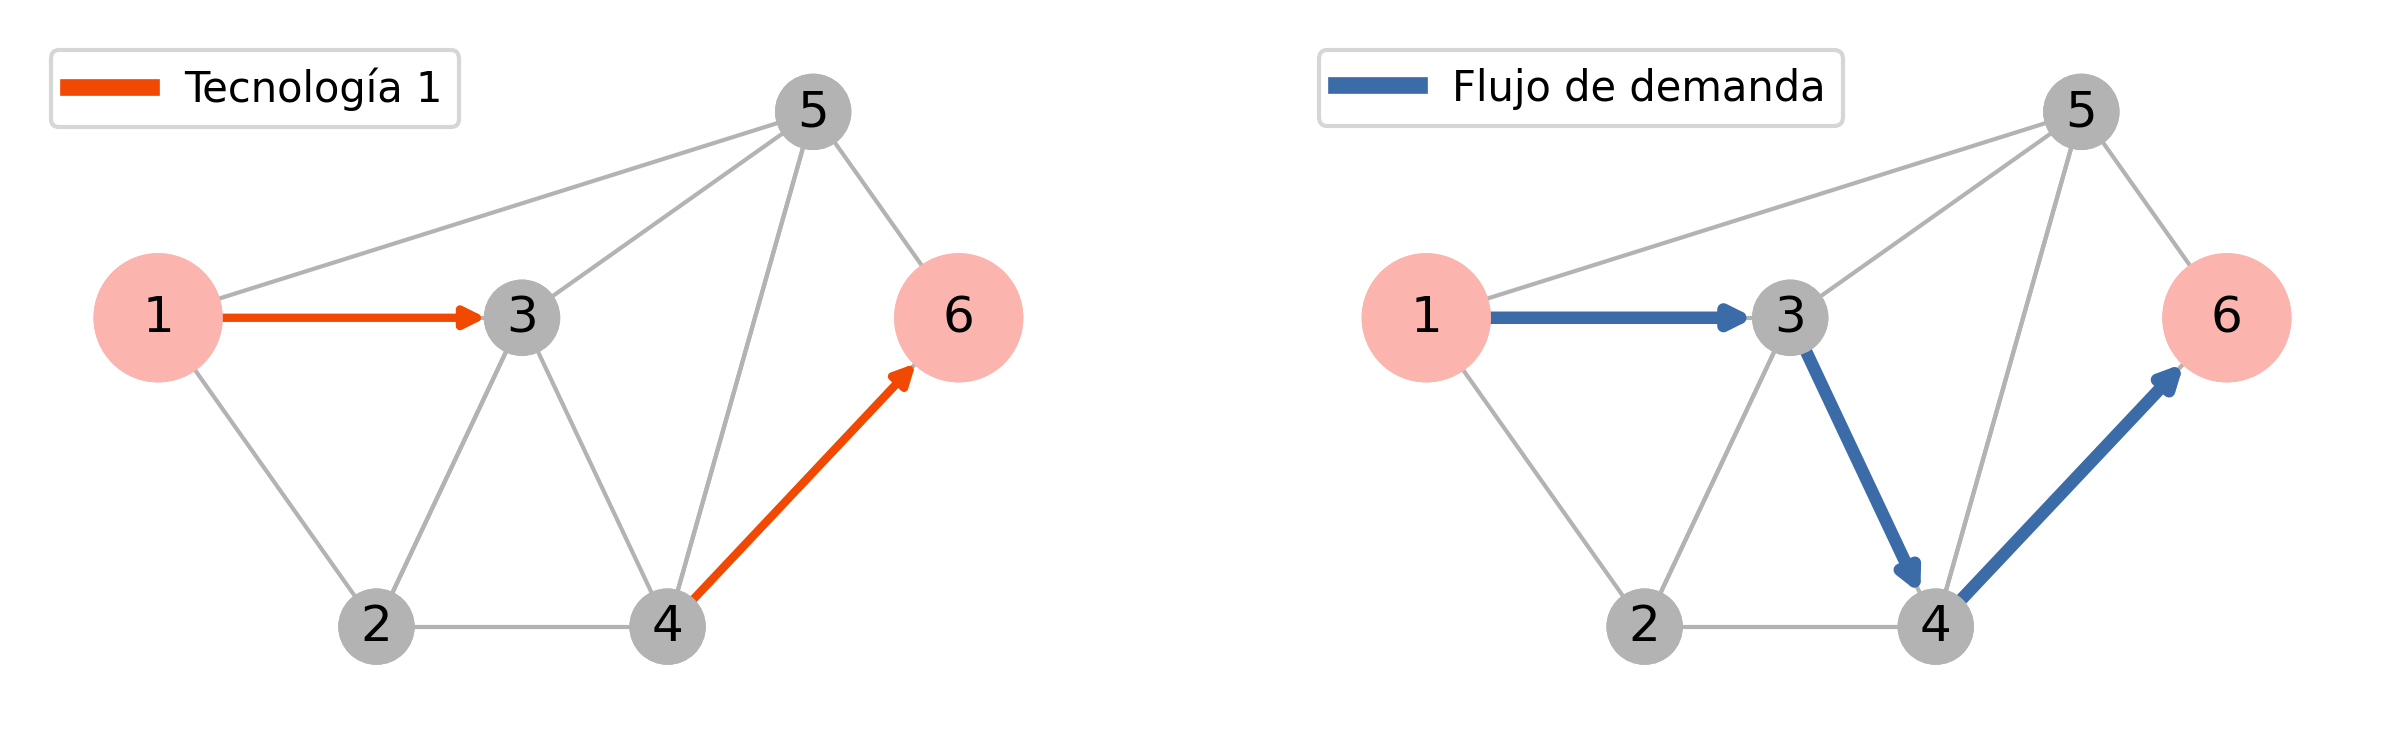
\includegraphics[width=\linewidth]{../resources/example_2_sol_v2.png}
  \caption{Representación de la solución S. A la izquierda se resaltan los arcos donde se construye la tecnología 1. A la derecha se observa el camino más corto sobre la red resultante.}
  \label{fig:example2solv2}
\end{figure}

\begin{figure}[h!]
  \centering
  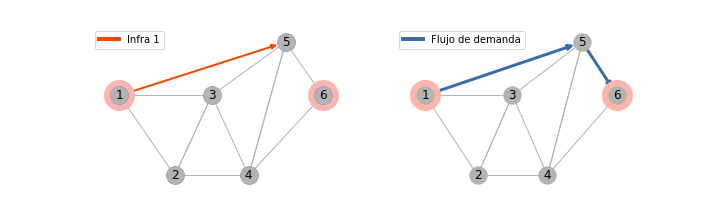
\includegraphics[width=\linewidth]{../resources/example_2_sol_v1.png}
  \caption{Solución SM. A la izquierda se resalta el arco donde se construye la tecnología 1 mientras que a la derecha se muestra el camino más corto, que coincide con el de la red base.}
  \label{fig:example2solv1}
\end{figure}

\FloatBarrier
\section{Análisis experimental}

El procedimiento de validación experimental consistió en generar instancias aleatorias, solucionarlas con las diferentes versiones y verificar que se cumplan las condiciones sobre las soluciones. Las diferentes alternativas fueron sobre la formulación de un nivel, dadas por las dos implementaciones de las $f_k$, las dos versiones multiobjetivo y la versión de un único objetivo. Consideraremos en principio parámetros $\beta = 1$ y $\rho = 1$ dado que obtuvimos resultados correctos con esta asignación en una ronda de pruebas preliminares.

Utilizamos la instancia de Sioux-Falls como grafo base, dada su amplia adopción en literatura relativa al tema \parencite{Liu2019}, datos que dejamos disponibles en el Apéndice \ref{sect:siouxfallsdata}. El costo de usuario de la tecnología base se tomó igual al largo del arco así como el costo de construcción de la tecnología 1. Consideramos en total tres tipos de tecnologías incluyendo la base, es decir $I = \{0, 1, 2\}$. Los costos de usuario y construcción se calcularon a partir de los costos de usuario base y de construcción para la tecnología 1, respetando la hipótesis de que a mayor nivel de tecnología mayor menor es el costo de usuario y mayor el de construcción. Este cálculo lo explicamos en la sección \ref{sect:dataspecification} y también lo dejamos especificado en el Apéndice \ref{sect:costcalculation}, página \pageref{sect:costcalculation}.

Para cada instancia, se sortearon entre 1 y 14 pares origen-destino y entre 2 y 10 valores de $P$ y $Q$ aleatorios cumpliendo con la hipótesis de modelar una función decreciente.
De esta manera generamos y probaron 1000 instancias para cada una de las seis variantes de las formulaciones. Nos interesa verificar si las soluciones cumplen con las características definidas en \ref{sect:solutioncharacteristics}, a saber: 1) que el costo de los caminos más cortos sobre la red resultante, es decir con infraestructura de ciclovía, es menor o igual al costo sobre la red sin infraestructura; 2) que el presupuesto excedente no es suficiente para construir infraestructura que mejore el costo del camino más corto de algún par origen-destino; 3) y que el costo del camino más corto sobre la red resultante no induce una demanda transferida distinta de la resultante. Ademas fue de nuestro interés comparar los valores de demanda transferida total y tiempos de ejecución.

\FloatBarrier
\subsection{Resultados}

\begin{table}[h!]
  \centering
  \begin{tabular}{cccSS}
    \toprule
      \shortstack{Versión \\ formulación} & Versión $f_k$ & Multiobj. & {Cant. Incump.} & \shortstack{Tiempo \\ Promedio (s)} \\
    \midrule
    v1 & v2 & 1  & 0   & 9,34    \\
    v2 & v2 & No & 76  & 22,94   \\
    v3 & v1 & 1  & 0   & 539,78  \\
    v4 & v1 & No & 67  & 495,80  \\
    v5 & v2 & 2  & 0   & 11,92   \\
    v6 & v1 & 2  & 0   & 283,93  \\
    \bottomrule
  \end{tabular}
  \caption{Comparativa agregada de ejecuciones sobre instancias aleatorias utilizando la red Sioux-Falls. La columna Multiobjetivo indica que versión multiobjetivo utilizada o si fue de un único objetivo (valor No). Los incumplimientos de una solución fueron computados en una unidad si la solución no cumplía al menos uno de las condiciones. En las versiones v2 y v4 los incumplimientos detectados corresponden únicamente a la condición \ref{budgetexcess} de las características de una solución.}\label{table:resumenejecuciones}
\end{table}

En las pruebas no detectamos diferencias en términos de los valores de demanda transferida total entre las diferentes formulaciones a excepción de una instancia. En las versiones v1 y v3, encontramos que la presencia de variables $r_{kj}$ en el objetivo puede resultar en una solución que induce menor valor de demanda transferida total en comparación a las otras formulaciones cuando se cumple que el valor de demanda transferida para un par origen-destino $k$ es comparable a la magnitud de $r_{kj}$, dado que $z_{kj}$ está activa. Por ejemplo, si para un par origen-destino se puede optimizar el camino más corto de manera de transferir cierta cantidad de demanda adicional, pero esto afecta la variable $r_{kj}$ de manera que la diferencia con el siguiente punto de quiebre es mayor que el nuevo salto en demanda transferida, entonces el modelo elige no realizar la mejora.

También observamos que en las versiones v2 y v4, que optimizan un único objetivo, se ve afectada en algunos casos la validez del ítem \ref{budgetexcess} de la característica de una solución. Esto se explica en casos en que la construcción de infraestructura en un arco puede mejorar el costo del camino más corto, pero no lo suficiente para afectar la cantidad de demanda transferida, lo cual implica que las decisiones de las tecnologías a construir pueda ser peor que en las otras variantes en el sentido del costo del camino más corto, como mostramos en el ejemplo \ref{sect:example2}. A diferencia del ejemplo, sin embargo, el presupuesto excedente es suficientemente para mejorar el camino de algún par origen-destino, lo que causa el incumplimiento.

A pesar de la diferencia encontrada en el valor de demanda transferida en un caso para las versiones v1 y v3, consideramos que aquellas multiobjetivo son las candidatas a ser elegidas como versión final dado que nos interesa tanto el valor objetivo como las decisiones en términos de la infraestructura ciclovía. Las diferencias en los valores de demanda transferida pueden ser corregidas como mostramos a continuación en una siguiente ronda de ejecuciones ajustando el peso $\beta$ del objetivo secundario.

El siguiente aspecto que tuvimos en cuenta es el tiempo de ejecución. El tiempo de ejecución promedio nos da una medida gruesa para comparar y descartar algunas versiones, considerando que las instancias de prueba son chicas y deberían ser de fácil resolución\footnote{El ser fácil está directamente relacionado a la cantidad de tiempo.}. Las versiones v3, v4 y v6, que utilizan la formulación v1 de $f_k$ tienen un tiempo de ejecución promedio significativamente más alto que las demás (Tabla \ref{table:resumenejecuciones}), que utilizan la otra versión. Nos interesó determinar si esta diferencia se da por algún tipo de instancia particular y si alguna versión se desempeña mejor en términos de tiempo de ejecución cuando quitamos las posibles instancias anormales en caso de que existan. En la Figura \ref{fig:runtimecomparison} se puede comparar el tiempo de ejecución de las versiones en todas instancias ejecutadas. Las versiones con mayor tiempo de ejecución promedio (v3, v4 y v6) muestran un peor comportamiento en general en comparación con las otras. También comparamos las dos versiones con menor tiempo promedio de ejecución, donde observamos que la v1 es en la mayoría de los casos la más rápida. Para las instancias más sencillas (primeros tres quintiles de las instancias, ver Figura \ref{fig:firstfourquintiles}), los tiempos de ejecución no varían demasiado entre formulaciones y solo hacia el cuarto quintil se notan diferencias aunque estas son de algunos segundos.

\begin{figure}[h!]
  \centering
  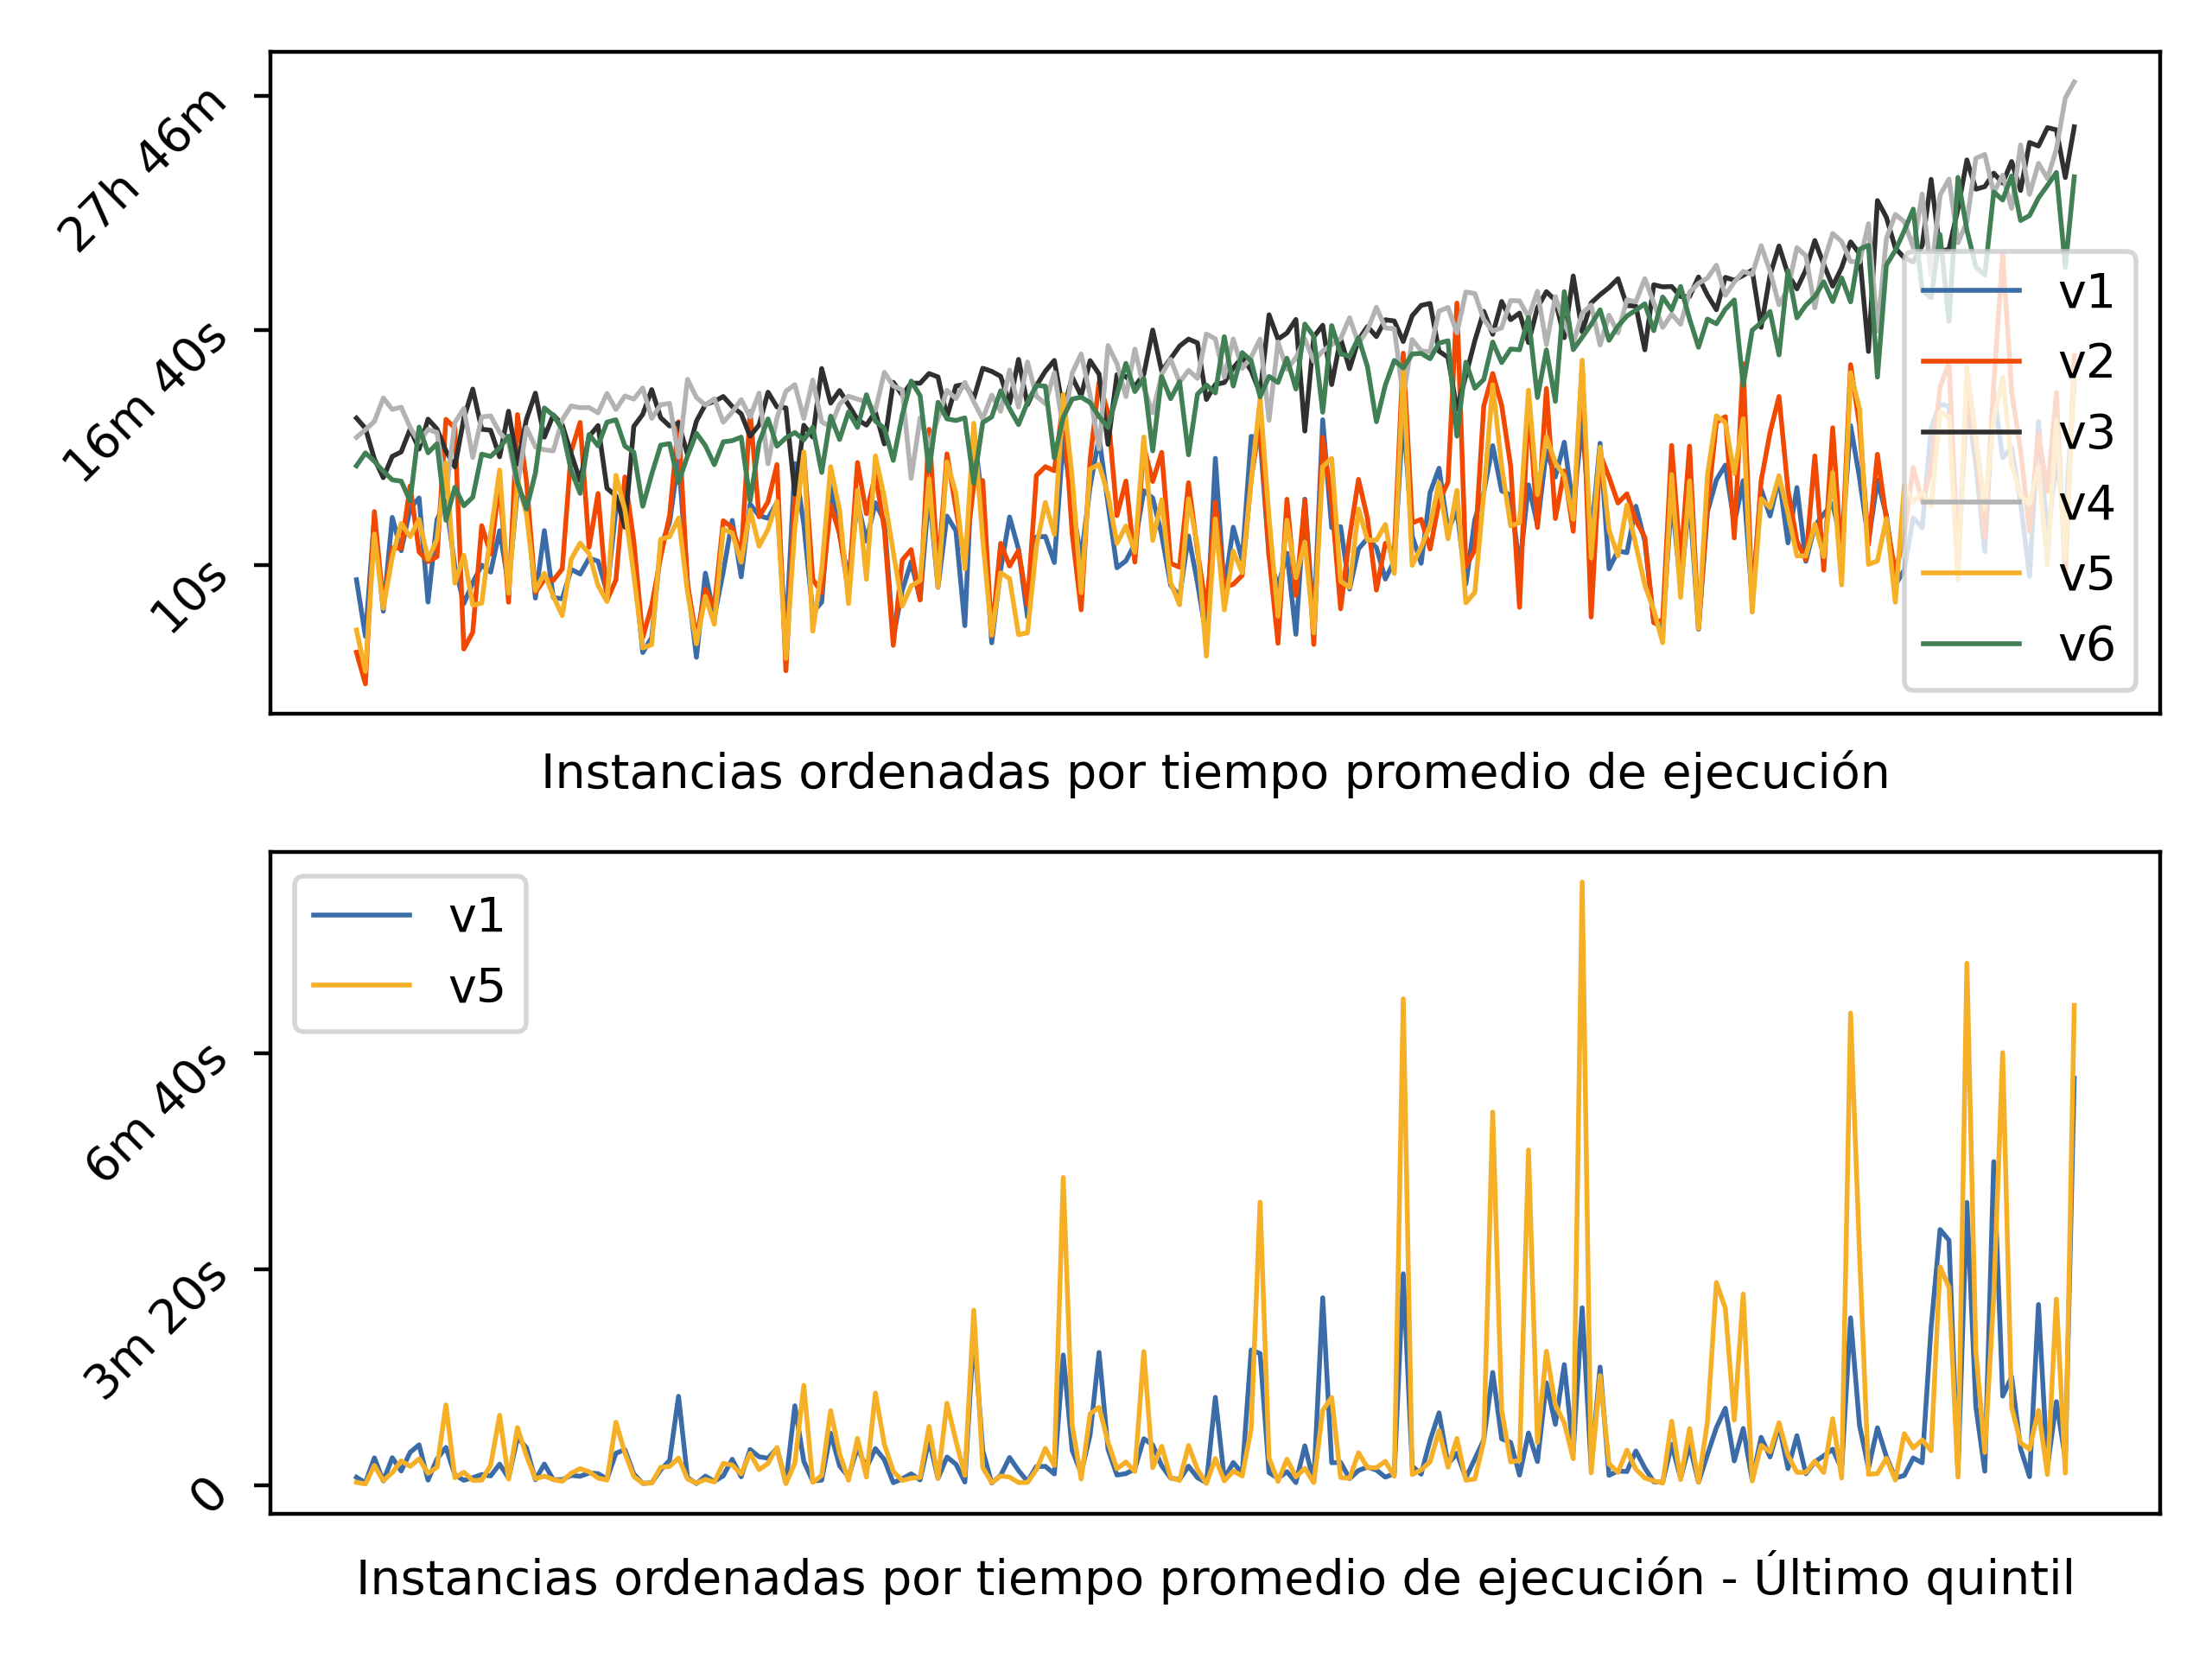
\includegraphics[width=12cm]{../resources/run_time_comparison.png}
  \caption{Comparativa del tiempo de ejecución de todas las versiones. Las instancias, en las abscisas, fueron ordenadas de forma creciente según el tiempo promedio de ejecución de todas las versiones. En la gráfica superior, la escala es logarítmica, dado que los valores a comparar oscilan entre pocos segundos y casi treinta horas. En la segunda gráfica la escala es lineal, tomamos la última quinta parte de las instancias ordenadas y las dos versiones con menor tiempo de ejecución para mostrar de manera más legible la escasa diferencia entre ellas en las instancias más difíciles.}
  \label{fig:runtimecomparison}
\end{figure}

\begin{figure}[h!]
  \centering
  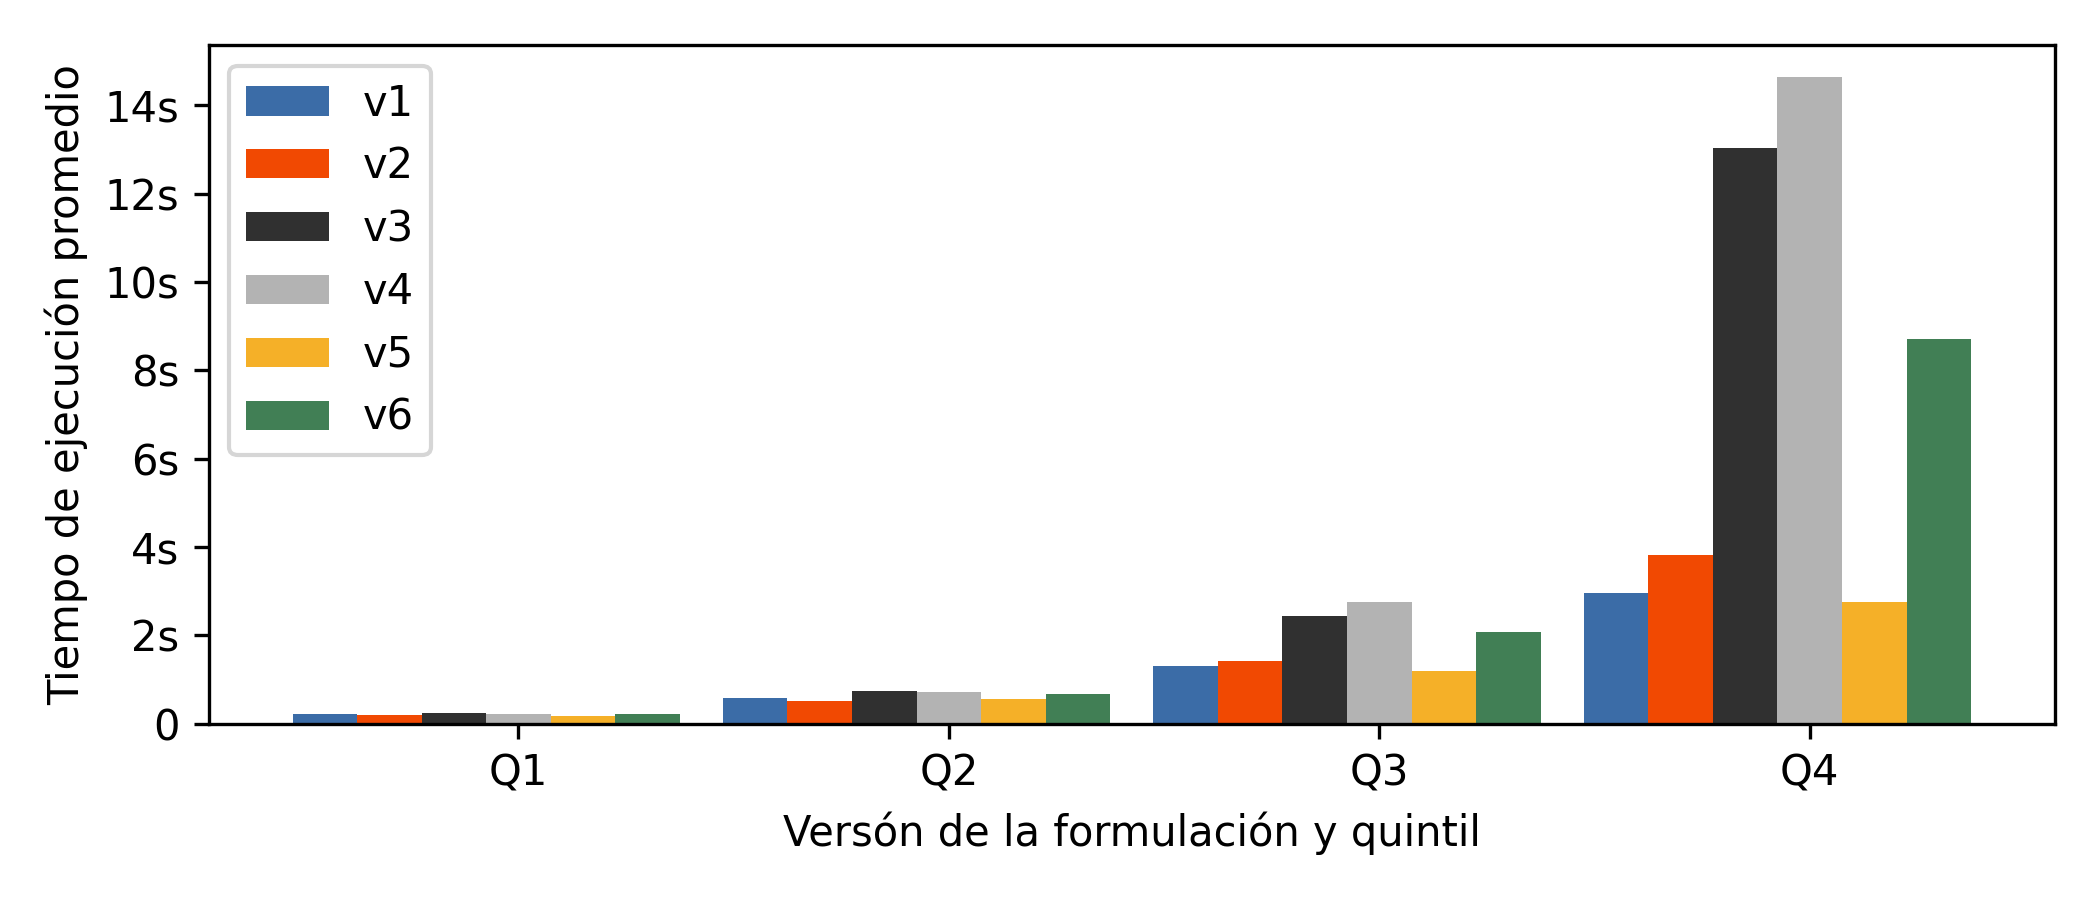
\includegraphics[width=12cm]{../resources/run_time_comparison_by_quintile.png}
    \caption{Comparativa del tiempo de ejecución de todas las versiones en tiempo promedio para los cuatro primeros quintiles. El tiempo promedio considerado es acumulado sobre los quintiles anteriores. El último quintil está omitido dado que los tiempos de ejecución se disparan para algunas instancias.}
  \label{fig:firstfourquintiles}
\end{figure}

Para solucionar la diferencia en demanda transferida cambiamos el valor del parámetro $\beta$ en (\ref{eq:multipleobj1}) de manera que se disminuye el efecto de las variables de $r_{kj}$ en la función objetivo de la formulación v1. El nuevo valor de $\beta$ es calculado para cada instancia y corresponde al factor mínimo entre los valores que hacen, para cada par origen-destino, que el costo del camino más corto para dicho par sea menor a la menor cantidad de demanda que se transfiere de un punto de quiebre a otro. Es decir, para cada $k \in OD$, buscamos un número $\beta_k$ que satisfaga: $\beta_k W_k \leq \min_{j \in J \setminus \{0\}} \{ P_{kj} - P_{k(j-1)} \}$, donde $W_k$ es el costo del camino más corto sobre el grafo base para el par origen-destino $k$. Luego tomamos $\beta = \min_{k \in OD} \{\beta_k\}$.

Ejecutamos nuevas pruebas comparando las tres versiones más rápidas: v1, v2 y v5. Esta vez generamos 1000 nuevas instancias aleatorias con cuatro tecnologías, lo que le da mayor complejidad. Nótese que si bien la v2 tiene incumplimientos, estos no implican que las soluciones sean erróneas a los efectos de la demanda transferida total.

% La versión v1 modificada sobre las instancias de la primera ronda no genero soluciones con incumplimientos y su tiempo de ejecución promedio
% fue 10,31 segundos

\begin{table}[h!]
  \centering
  \begin{tabular}{cSS}
    \toprule
      Versión & {Cant. Incump.} & \shortstack{Tiempo \\ Promedio (s)} \\
    \midrule
    v1 & 0   & 79,71   \\
    v2 & 119 & 282,11  \\
    v5 & 0   & 207,50  \\
    \bottomrule
  \end{tabular}
  \caption{Comparativa agregada de ejecuciones sobre la segunda ronda de instancias aleatorias sobre la red de Sioux-Falls.}\label{table:resumenreejecuciones}
\end{table}

Los nuevos resultados se encuentran resumidos en la Tabla \ref{table:resumenreejecuciones}. En esta ronda de pruebas no detectamos diferencias en términos de la demanda transferida total y verificamos que la diferencia en la instancia problemática de la primera ronda fue solucionada. En términos de tiempo de ejecución, los resultados se encuentran en las Figuras \ref{fig:runtimecomparisonrerun} y \ref{fig:firstfourquintilesrerun}. Observamos que se mantiene el comportamiento de la ronda de pruebas anterior y la v1 sigue siendo más rápida. También observamos que el desempeño de v5 se degradó de peor manera. Dados los resultados, decidimos continuar el resto de este trabajo con la versión v1 de la formulación.

\begin{figure}[h!]
  \centering
  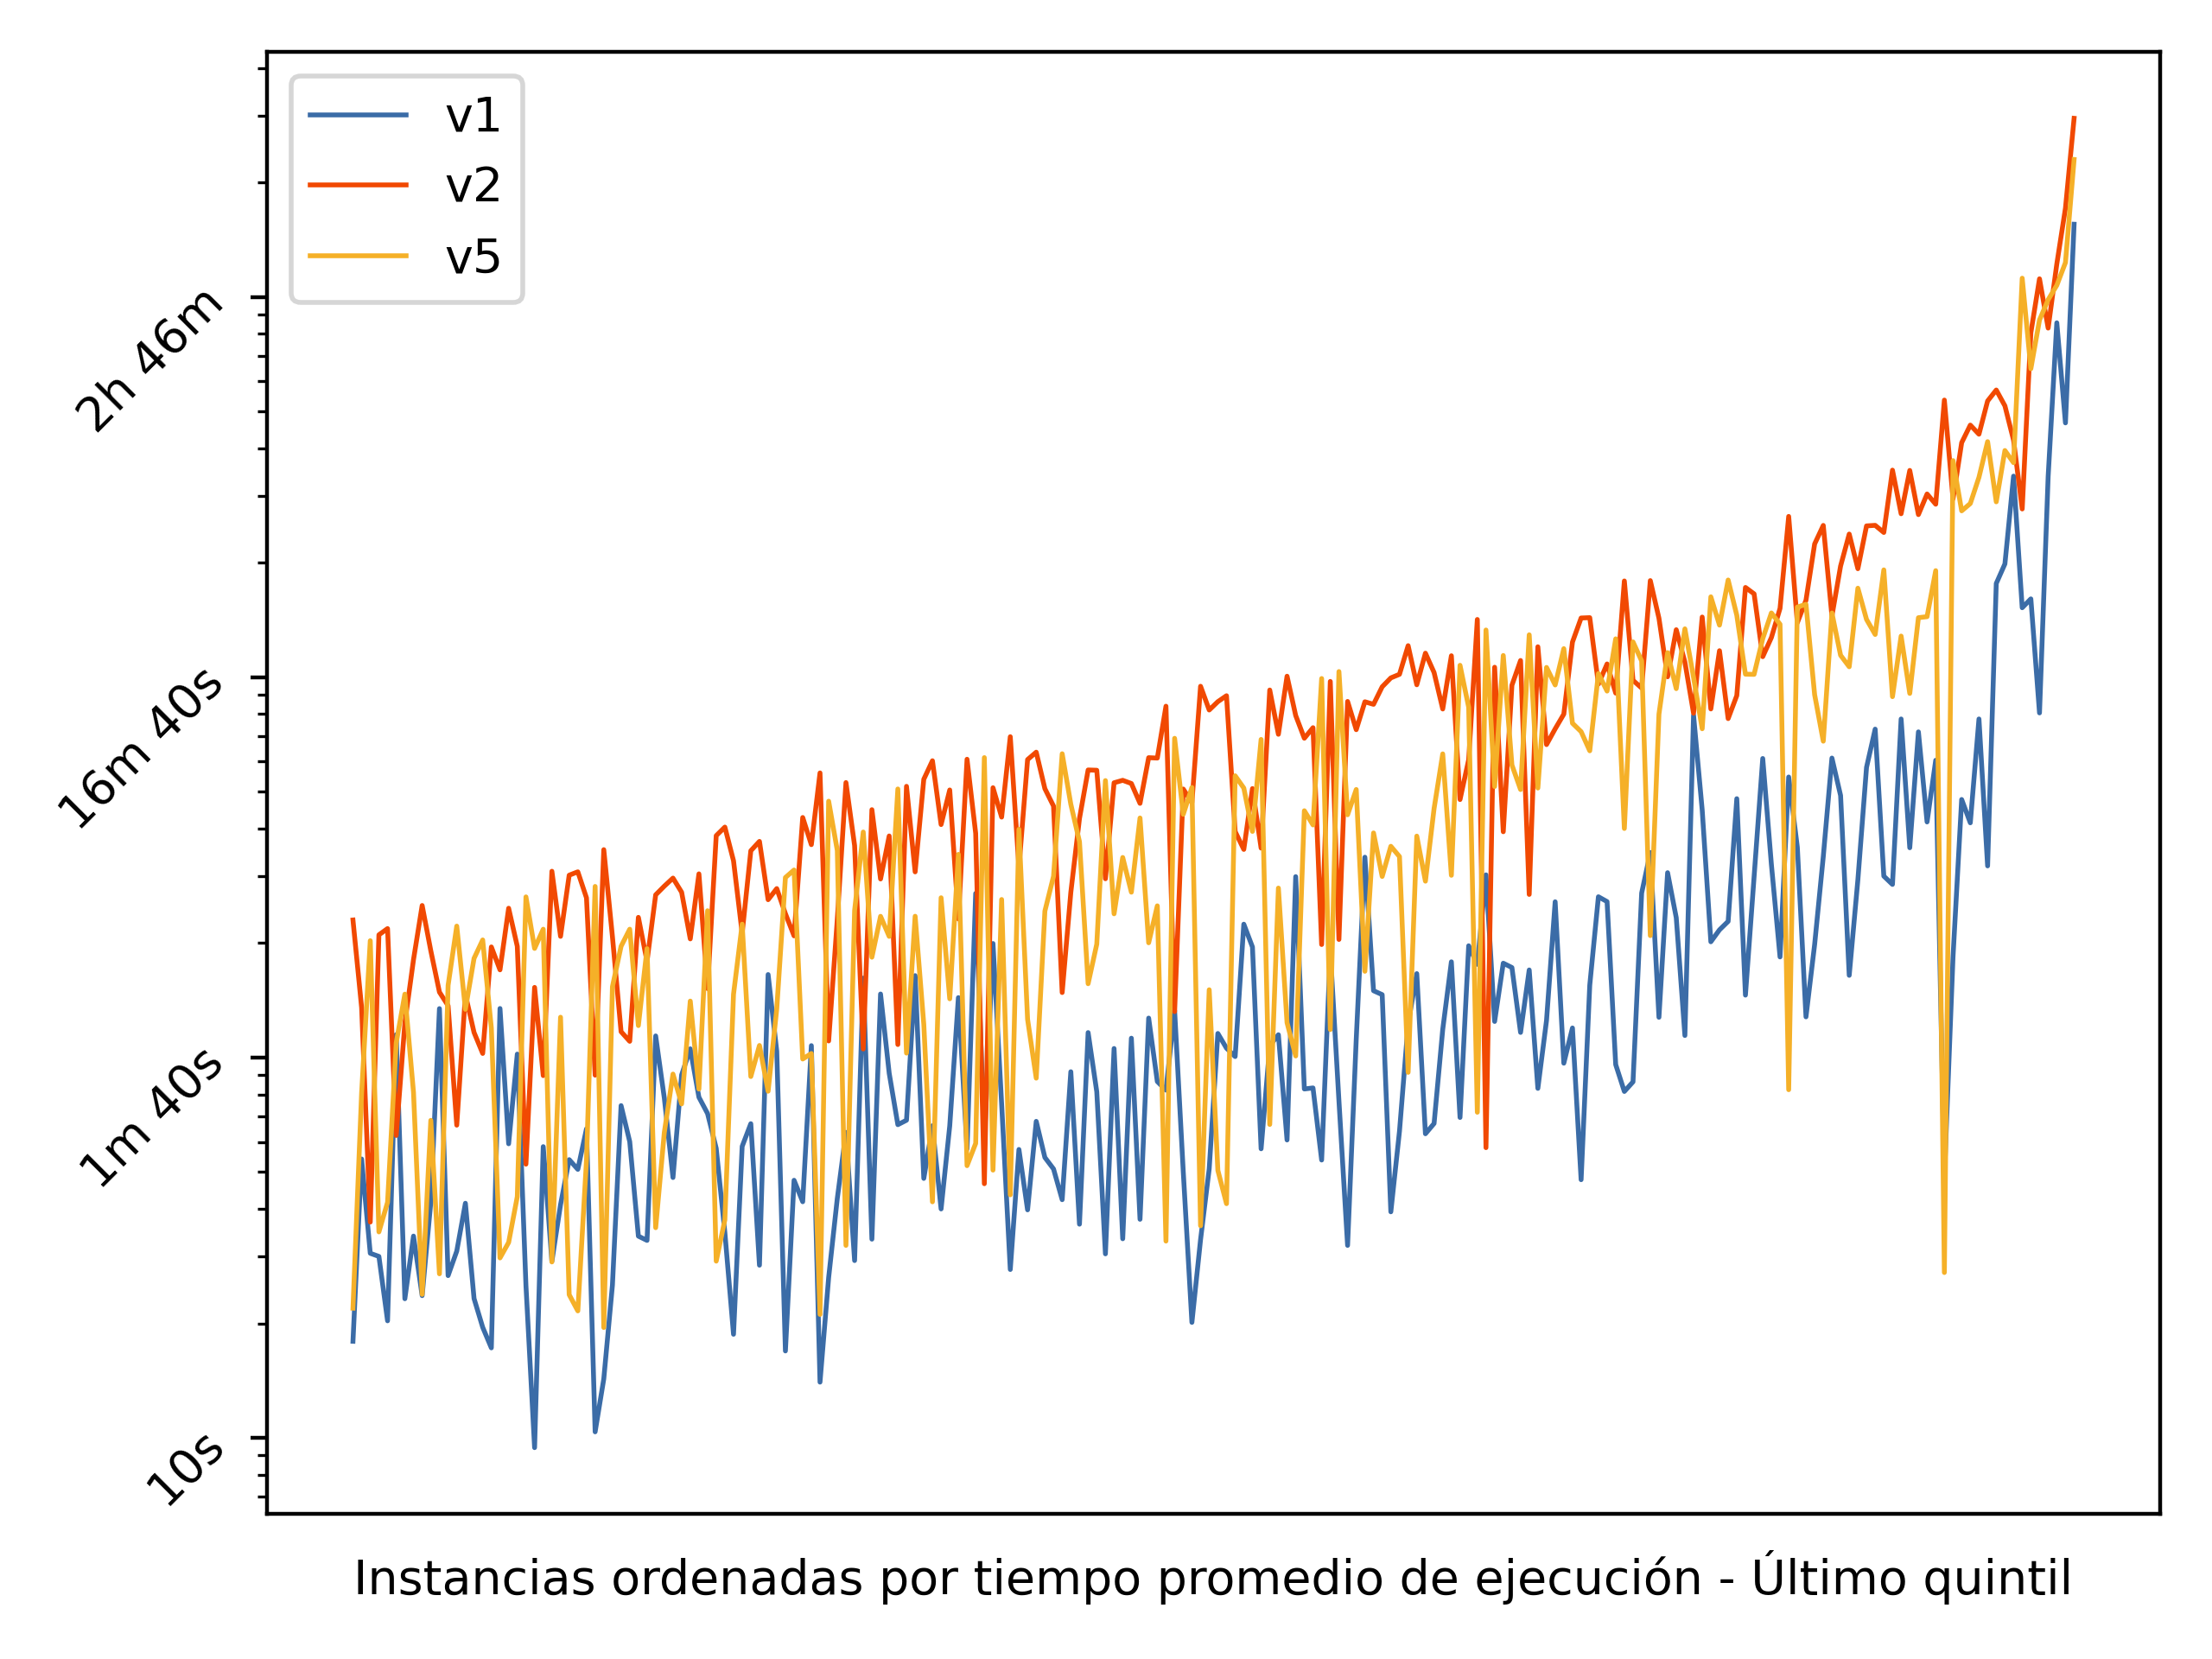
\includegraphics[width=12cm]{../resources/run_time_comparison_rerun.png}
  \caption{Comparativa del tiempo de ejecución sobre la segunda ronda de instancias en los tres mejores modelos de la primera ronda. La escala es logarítmica en el eje de las ordenadas.} \label{fig:runtimecomparisonrerun}
\end{figure}

\begin{figure}[h!]
  \centering
  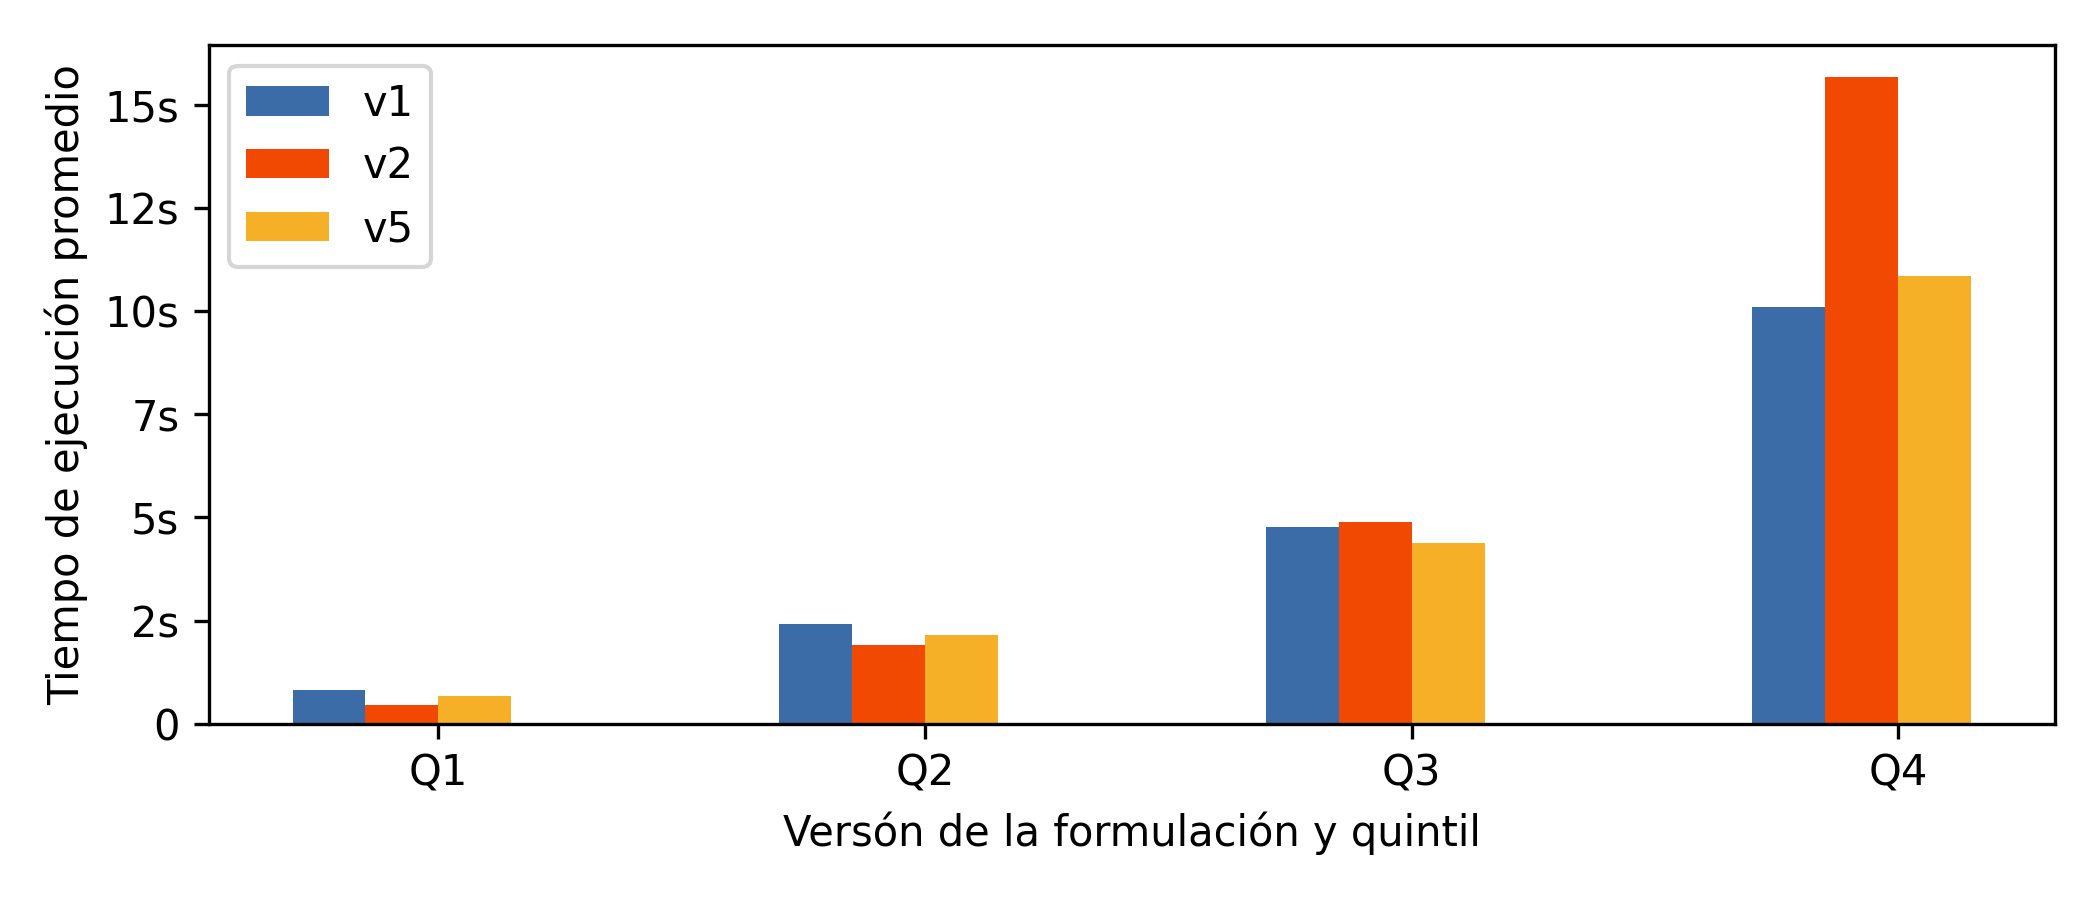
\includegraphics[width=12cm]{../resources/run_time_comparison_by_quintile_rerun.png}
  \caption{Comparativa del tiempo de ejecución sobre la segunda ronda de instancias en los cuatro primeros quintiles. Las instancias fueron ordenadas por tiempo promedio de ejecución.} \label{fig:firstfourquintilesrerun}
\end{figure}

  \chapter{Experimentos computacionales}
\label{sect:problemresults}

En este capítulo ponemos a prueba el modelo resultante del capitulo \ref{sect:problemresolution}. Para empezar estudiamos el comportamiento del modelo frente a perturbaciones en alguno de sus parámetros específicos del problema, es decir modelado de la transferencia de demanda, presupuesto y tecnologías de ciclovías, sobre la red de Sioux-Falls de manera de poder realizar pruebas en tiempo razonable. En particular, analizamos los resultados respecto a la demanda transferida total y a las decisiones que se toman sobre las ciclovías a construir. Luego aplicamos el modelo a una instancia de tamaño realista que modela la ciudad de Montevideo. Antes de presentar los resultados, discutimos el criterio con el que elegimos los valores de costos de construcción de las diferentes tecnologías de ciclovía, costos de usuario por tecnología, funciones de transferencia de demanda y valores de presupuesto.

\section{Especificación de datos}
\label{sect:dataspecification}

Nuestro problema requiere la disponibilidad de parámetros que en la práctica no son fáciles de estimar de forma realista como los costos usuario y construcción por tipo de tecnología y transferencia de demanda en función del costo de usuario. En esta sección definimos algunos criterios que utilizamos para especificarlos en base a trabajos de la literatura. En la siguiente, analizamos qué efectos tienen las perturbaciones sobre las soluciones.

La cantidad y tipos de tecnologías de ciclovía varían de un contexto a otro tanto en su disponibilidad como en sus costos y por lo tanto es difícil estimar estos últimos de manera general sin llegar a un análisis caso a caso. Por ejemplo en la ciudad de Montevideo podemos encontrar tres tipos \footnote{Mapa interactivo: \url{https://montevideo.gub.uy/mapa-montevideo-en-bici}}: el más básico consiste en imponer un límite superior de velocidad para los vehículos automotores (30 km/h) y cartelería resaltando cierta calle o zona como habilitada para el tránsito en bicicleta. Un segundo tipo consiste en utilizar una fracción de la calle como senda específica para bicicletas que puede ir en uno o ambos sentidos. Y el tercer tipo consta de una bicisenda construida específicamente para bicicletas generalmente en canteros y parques.

Los costos de construcción pueden variar según la ubicación y tipo de ciclovía, congestión del área de la ciudad y su afectación por las obras, precios de insumos externos como el petróleo y cuestiones logísticas como reubicación de paradas de ómnibus y señales de tránsito, entre otros aspectos. Se puede encontrar información al respecto en el análisis \cite{typicalcostsofcylcing} que presenta diversos tipos de tecnologías y los principales factores que afectan el costo de construcción como trabajo dentro de un programa de incentivo del transporte en bicicleta en Inglaterra. En base a dicho trabajo simplificamos y generalizamos el cálculo de los cotos de construcción para cada tipo de tecnologías de la siguiente manera: la tecnología de tipo $i + 1$ cuesta el doble que la tecnología de tipo $i$. Esto también es consistente con la información disponible para la ciudad de Montevideo \footnote{Información obtenida por comunicación personal con la Intendencia de Montevideo.}. Entonces, sean $l_a$ el largo del arco $a \in A$ y $CC_i$ el costo de construcción de la tecnología $i \in I$ por unidad de distancia, los costos de construcción por tecnología y arco quedan: $H_{ai} = l_a CC_i, \forall a \in A, i \in I$; donde $CC_i = 2 * CC_{i-1}, \forall i > 2$; $CC_1 = 1$ y $CC_0 = 0$.

Por otro lado, los costos de usuario de atravesar un arco varían en la práctica dependiendo de factores como ancho de la vía, pavimento, volumen y velocidad del tránsito, entre otros, que a su vez se ponderan por el largo del arco. En el documento \cite{blos2007} podemos encontrar el concepto de {\it Bicycle Level of Service} (BLOS), muy utilizado en la literatura, que agrupa estas consideraciones bajo un único valor. Para el cálculo del BLOS se tienen en cuenta los distintos aspectos que cuantificados en indicadores, son luego utilizados en una fórmula para calcular el puntaje de BLOS que se estratifican en 6 niveles del A al F.

Los aspectos que se consideran son los siguientes:

\begin{enumerate}
  \item{Ancho promedio de la banquina, presencia de ciclovía, porcentaje de la vía ocupada por estacionamiento}
  \item{Límite de velocidad de vehículos motorizados}
  \item{Volumen promedio de los vehículos motorizados}
  \item{Porcentaje de tránsito pesado (camiones)}
  \item{Condición del pavimento}
\end{enumerate}

\begin{table}[h!]
  \centering
  \begin{tabular}{cccc}
    \toprule
      Nivel & Puntaje BLOS & Tecnología & \shortstack{Proporción de mejora \\ sobre costo base} \\
    \midrule
      A     & $\leq 1.5$   & 5              & 0,4   \\
      B     & 1,5-2,5      & 4              & 0,52  \\
      C     & 2,5-3,5      & 3              & 0,64  \\
      D     & 3,5-4,5      & 2              & 0,76  \\
      E     & 4,5-5,5      & 1              & 0,88  \\
      F     & > 5,5        & 0              & 1     \\
    \bottomrule
  \end{tabular}
  \caption{Niveles de servicio definidos en el BLOS, menor puntaje BLOS representa mejores condiciones para el usuario. Para cada nivel definimos un tipo de tecnología y su correspondiente proporción de mejora sobre la tecnología base.}\label{table:blosscores}
\end{table}

En esta tesis nos enfocamos en la planificación estratégica de una red ciclovías sin asumir aspectos detallados para su diseño por lo tango ignoramos algunos factores tomados en cuenta para el cálculo del BLOS. Mediante la construcción de infraestructura de ciclovía solo podemos mejorar alguno de los siguientes aspectos: límite de velocidad de vehiculos motorizados, presencia de ciclovías y condiciones del pavimento.

Tomando como base el puntaje de BLOS estratificado de la Tabla \ref{table:blosscores}, siguiendo el cálculo en \cite{baya2021}, podemos traducir de forma aproximada los puntajes de BLOS a proporción de mejora sobre la tecnología base o red de calles utilizando la función $C_{infra}(i) = {28 - 3 (i + 1) \over 25}$ donde $i \in I = \{0,1,2,\ldots\}$ es el tipo de tecnología. Suponiendo que el nivel F de la escala de BLOS corresponde a tecnología base (o tecnología 0), la proporción de mejora de las tecnologías A-E correspondientes a los tipos de tecnologías 5,4,3,2 y 1 respectivamente se pueden observar en la misma tabla.

Incurrimos a la simplificación de considerar, al definir una instancia, la cantidad $T$ de tipos tecnologías posibles a utilizar y no cuáles, de manera que los tipos de tecnología utilizables sean $I = \{0,.., T - 1\}$. Dada una instancia del problema, llamamos $m$ a la proporción de mejora máxima que puede dar la mejor tecnología de entre las disponibles, es decir $m = C_{infra}(T - 1)$. El valor $m$ es de utilidad al definir las funciones de transferencia de demanda como veremos a continuación.

Respecto al comportamiento de los usuarios, suponemos que la demanda de todos los pares origen-destino se comporta de igual manera, lo cual tiene sentido al considerar una población determinada. Esto reduce la necesidad de especificar $|OD|$ funciones de transferencias de demanda a una sola. Es decir, para cada par origen destino $k$, tenemos que $f_k(w_k) = f({w_k \over S^{best}_k})d_k$, donde $d_k$ es la demanda máxima que se puede transferir, $S^{best}_k$ es el costo del camino más corto sobre la tecnología base y $f: [m, 1] \rightarrow [0, 1]$ modela la proporción de demanda transferida en función de la proporción del nuevo costo sobre el costo base $S^{best}_k$.

Partimos de \cite{shwe2014} en el que analizando una extensiva encuesta realizada en varios países aproxima la proporción de viajes hechos en bicicleta y el largo de infraestructura de ciclovía per cápita en la ciudad a una relación lineal. Tomando este resultado, utilizamos una función lineal decreciente como función de transferencia de referencia. Como alternativa, en \cite{ortuz2011} se menciona que el comportamiento de la demanda al momento de decidir entre dos modos se comporta como una función con forma de S, logística o sigmoide, por lo que también consideramos una función logística en nuestras pruebas. Por completitud analizamos otras funciones que podrían considerarse razonables: una con concavidad estrictamente positiva y otra con concavidad estrictamente negativa en el intervalo $[m, 1]$. La definición explícita se encuentra en la Sección \ref{sect:fspecification}.

Establecer valores de presupuesto realistas depende altamente de las condiciones políticas y económicas de cada localidad. Podemos encontrar en \cite{rios2015} y \cite{shwe2014} que factores de cubrimiento de la red de ciclovías en una ciudad de entre 10\% y 40\% del total de la red de calles de una ciudad están dentro de los parámetros normales. Seguimos este enfoque y especificamos el presupuesto como porcentaje del costo total de construir una infraestructura de ciclovía en toda la red tomando como referencia el costo de la tecnología 1, es decir la tecnología especializada más básica que sigue a la red de calles. Dado nuestro método para el cálculo de los costos de los tipos de tecnologías, esto implica que un presupuesto del 40\% es suficientemente para cubrir 20\% solo con la tecnología de tipo 2, 10\% solo con la tecnología de tipo 3; y en general un factor de $F\%$ cubre ${F \over {2^{i - 1}}}\%$ de la tecnología $i \in \{1,..,5\}$.

Finalmente, usamos el largo de los arcos como costo de usuario y costo de construcción de la tecnología 1. Esto nos da una medida suficientemente simple y general como para usar en cualquier instancia.

\section{Especificación de funciones de transferencia de demanda}
\label{sect:fspecification}

Las funciones de transferencia de demanda probadas fueron cuatro, ver Figura \ref{fig:fcatalog}. Si bien las funciones fueron creadas para este trabajo, las versiones lineal y logística están basadas y son consistentes con los trabajos de \cite{shwe2014} y \cite{ortuz2011} respectivamente. Las versiones con concavidad negativa y positiva fueron creadas para complementar el estudio y están compuestas de funciones logísticas desplazadas de manera de lograr la concavidad deseada en el intervalo $[m, 1]$.

Las expresamos parametrizadas por $m$, correspondiente a la proporción de mejora máxima alcanzable por la mejor tecnología, ya que es el mínimo valor que tiene sentido. Definimos las funciones en $[m, 1] \rightarrow [0, 1]$ de la siguiente manera:

\begin{definition}
  Lineal
  \begin{align}
      f(x) = {x -1 \over m - 1}
  \end{align}
\end{definition}

\begin{definition}
  Logística
  \begin{align}
      f(x) = {1 \over 1 + e^{2k_m(x - ({1 + m \over 2}))}}
  \end{align}
\end{definition}

\begin{definition}
  Concavidad negativa.
  \begin{align}
      f(x) = {2 \over 1 + e^{k_m(x - 1)}} - 1
  \end{align}
\end{definition}

\begin{definition}
  Concavidad positiva.
  \begin{align}
      f(x) = {2 \over 1 + e^{k_m(x - m)}}
  \end{align}
\end{definition}

El parámetro $k_m$ determina la pendiente de las funciones basadas en la función logística y es utilizado para que los valores funcionales en los extremos de $(m, 1)$ estén cerca de $1$ y $0$ respectivamente. Fue determinado de manera experimental y se calcula como $k_m = {3 \over 1 - m}$. Al utilizar estas funciones fue necesario normalizar el codominio de manera que abarque el intervalo $[0, 1]$ dado que el parámetro $k_m$ no garantiza que esto suceda.

\begin{figure}[h!]
  \centering
  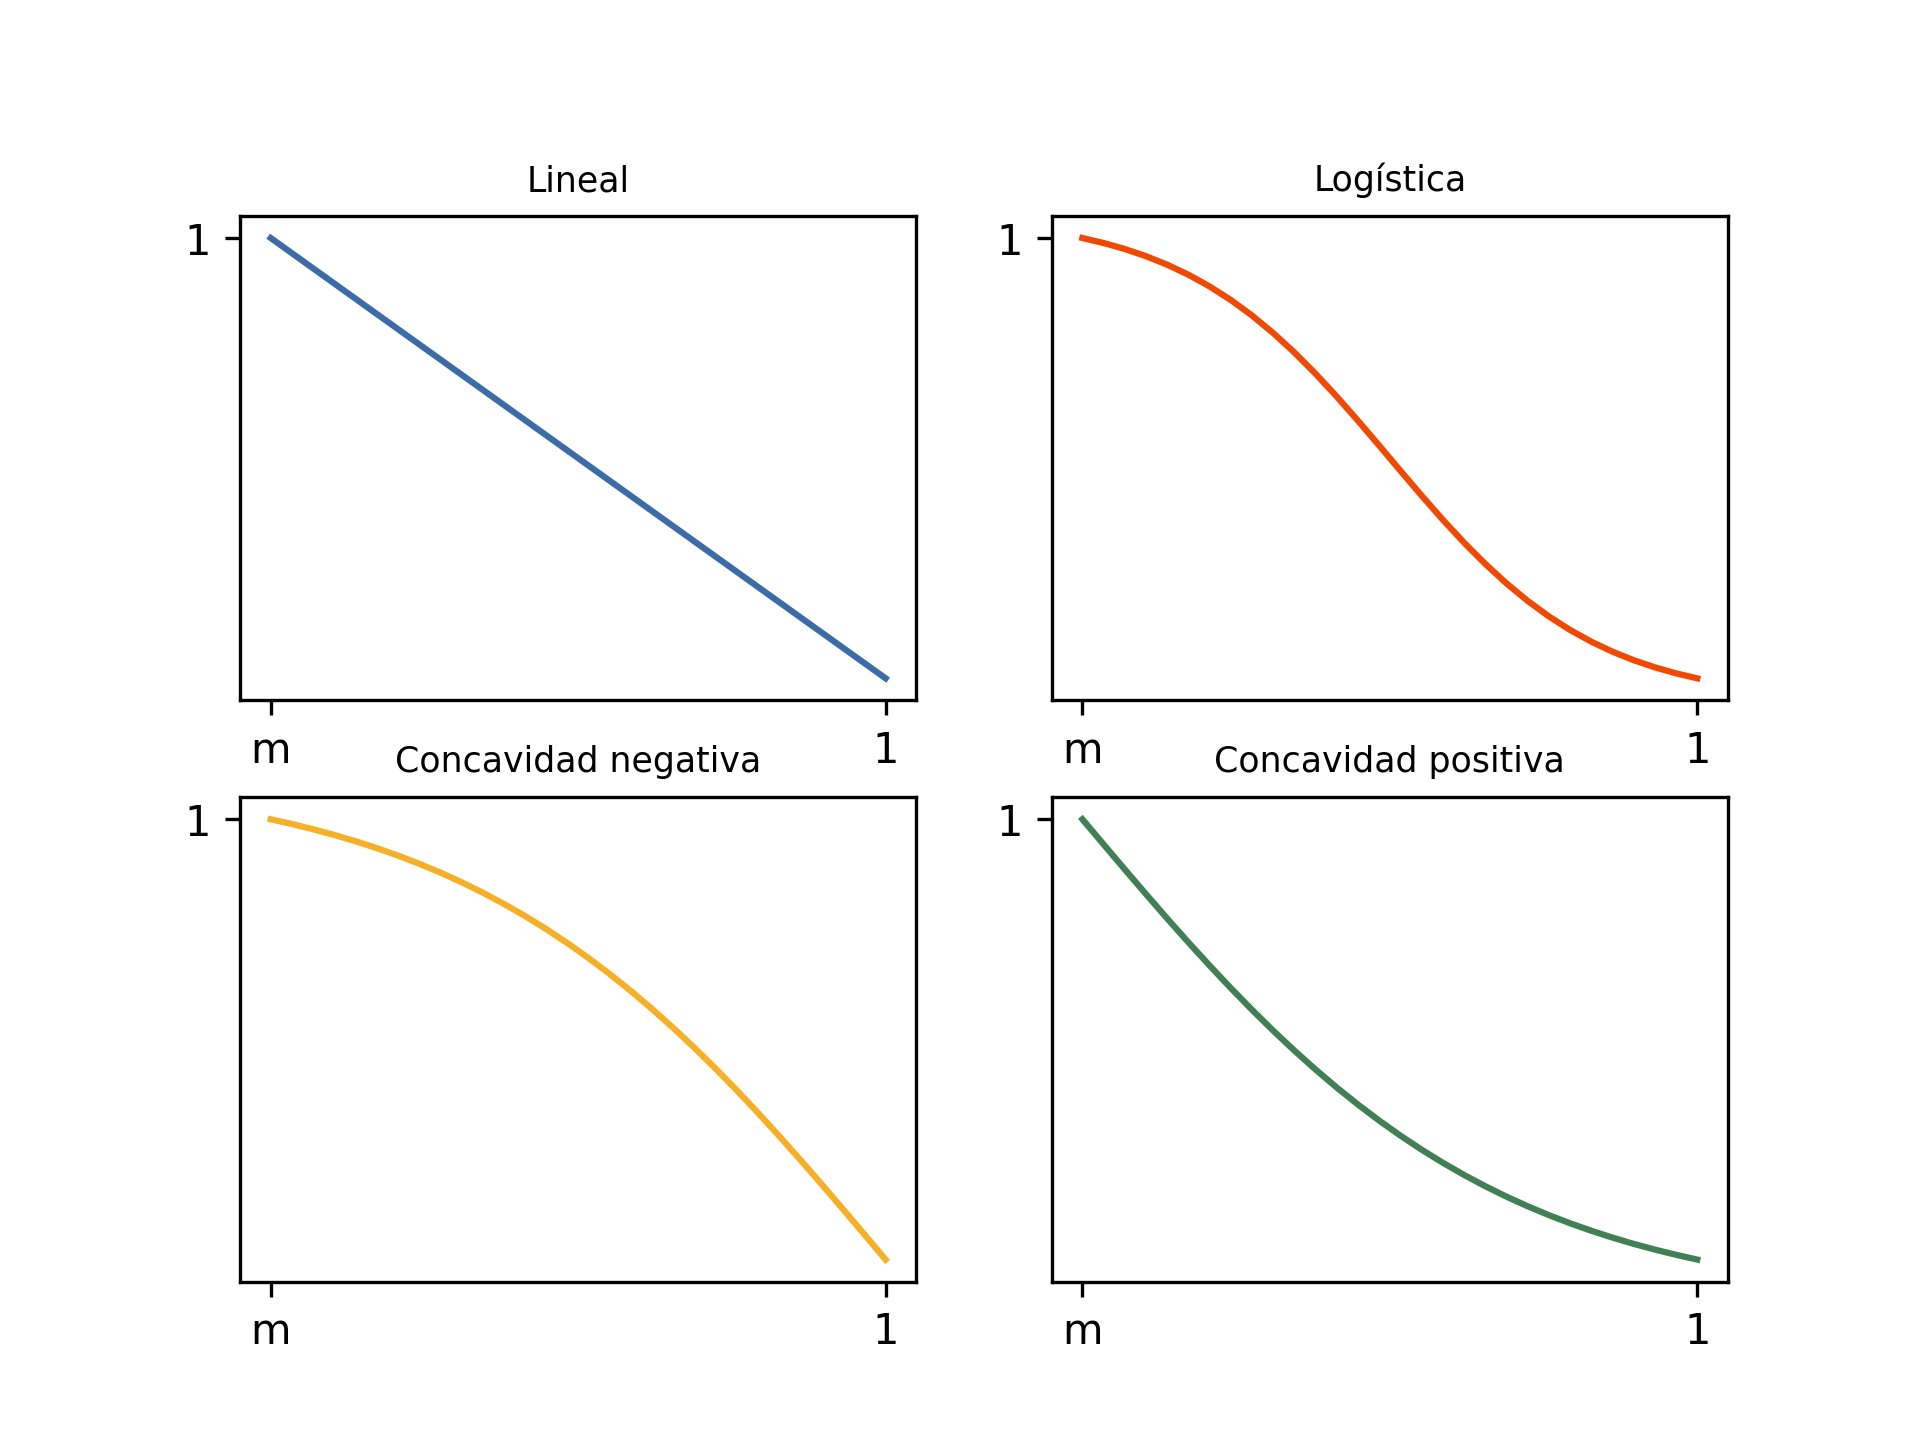
\includegraphics[width=10cm]{../resources/f_catalog.png}
    \caption{Catálogo de funciones usadas para modelar la transferencia de demanda a la bicicleta. El valor de $m$ varía según la tecnología de ciclovía utilizada y equivale a la proporción mínima alcanzada por la mejor tecnología utilizada, es decir $m = min_{i \in I} \{ C_{infra}(i) \}$.}
  \label{fig:fcatalog}
\end{figure}

\section{Análisis de sensibilidad}

Estudiamos el comportamiento del modelo frente a perturbaciones en alguno de sus parámetros. Utilizamos la red de Sioux-Falls nuevamente dado que es de un tamaño manejable para realizar todas las ejecuciones en tiempo razonable. Las perturbaciones las realizamos sobre los parámetros específicos del problema, dejando los datos de la red y matriz de demanda fijos. Estos son: puntos de quiebre, funciones de transferencia de demanda y presupuesto. Observar que los parámetros estudiados son de distinta naturaleza: mientras que los primeros dos son relativos al modelado del comportamiento de la demanda el último es una decisión exclusiva de la entidad planificadora. La matriz de demanda se toma de \cite{Liu2019}, con 22 pares origen-destino. Los datos de la red y matriz de demanda se encuentran en el Apéndice \ref{sect:siouxfallsdata}.

\FloatBarrier
\subsection{Perturbaciones}

Uno de nuestros objetivos es determinar cuáles son las perturbaciones, más allá de un incremento en el presupuesto, que resultan en mayores valores de demanda transferida total. Por un lado, la cantidad de tipos de tecnologías disponibles es determinante respecto a la mejora alcanzable en los caminos. Es de esperar que el modelo decida utilizar mejores tecnologías en los arcos con mayor flujo de demanda, tanto como el presupuesto y tipos de tecnologías disponibles lo permitan. En principio no hay razón para limitar este número a un valor distinto del mayor valor posible, a menos que el deterioro en el tiempo de ejecución lo haga necesario. Respecto a los puntos de quiebre, esperamos que una mayor granularidad aporte positivamente a nuestro objetivo, aunque, al igual que la cantidad de tipos de tecnologías, tendremos cuidado con deterioro en el desempeño.

Como instancia de referencia consideramos la red de Sioux-Falls y matriz de demanda antedicha y el siguiente conjunto de parámetros en base a la discusión de la sección anterior:

\begin{description}
  \item[Tecnologías de ciclovía]: 5 tipos de tecnologías además de la base.
  \item[Puntos de quiebre]: Función lineal de transferencia de demanda con 5 puntos de quiebre.
  \item[Presupuesto]: Factor de presupuesto del 80\%.
\end{description}

Las perturbaciones las realizamos sobre el conjunto de parámetros de la instancia de referencia aplicando una o dos perturbaciones por vez en lugar de ejecutar todas las posibles combinaciones de parámetros perturbados, ya que esto implicaría una mayor cantidad de instancias a estudiar.

En primer lugar analizamos la sensibilidad respecto al factor de presupuesto. Los valores utilizados son: 10\%, 80\%, 160\% y 320\%. El objetivo es observar si se cumple la simple intuición de que siempre a mayor presupuesto se obtienen mejores resultados y cómo es el comportamiento de la demanda transferida total respecto a los incrementos de presupuesto. También analizamos el efecto que tiene la cantidad de puntos de quiebre en los resultados, utilizando 5 y 20 puntos para cada presupuesto.

Luego, comparamos el resultado de aplicar diferentes funciones de transferencia de demanda y cómo afecta el hecho de utilizar distintas cantidades de puntos de quiebre. Utilizamos 5, 20 y 50 puntos de quiebre junto a las cuatro funciones mencionadas en la sección anterior (\ref{sect:dataspecification}). Definimos los puntos de manera que sean equidistantes en el codominio, es decir, si hay N puntos, de un punto al siguiente se obtiene una mejora de aproximadamente ${1 \over N - 1}$ en la proporción de demanda transferida.

Como resultado tenemos 36 instancias cuya representación pre simplificaciones en solver CPLEX son matrices que van desde un tamaño de 12597x12310 con 562 variables binarias hasta 14487x14290 con 1552 variables binarias.

\FloatBarrier
\subsection{Resultados}

Las instancias fueron ejecutadas con el solver CPLEX versión 12.8.0.0 en su configuración por defecto sobre una máquina Intel Core i9-9900K con 64GiB de RAM. Los resultados generales de las ejecuciones se encuentran en la Tabla \ref{table:sensibilityresults} y los datos sobre el uso del presupuesto, que luego comentaremos, en la Tabla \ref{table:sensibilitybudgetusage}.

Se puede observar que a mayor cantidad de puntos de quiebre, fijando la función de transferencia de demanda y el presupuesto, obtenemos mayor transferencia de demanda. Esto tiene sentido ya que la función de transferencia es representada de manera más precisa. También vemos que variar la cantidad de puntos de quiebre parece hacer variar el tiempo de ejecución en algunos casos, sin poderse determinar una relación general entre la cantidad y la complejidad resultante pero si podemos ver que fijando los otros parámetros y aumentando la cantidad de puntos de quiebre la complejidad aumenta. Por otro lado, observamos un fuerte impacto del modelado del comportamiento de la transferencia de demanda, es decir de cuál función se utiliza, sobre la demanda transferida. Esto nos confirma que es un aspecto importante del modelado, si bien las funciones consideradas en este caso pueden haber sido poco realistas o exageradas en sus curvaturas. Finalmente, vemos que la demanda transferida en función de la cantidad de presupuesto, fijando cantidad de puntos de quiebre y función de transferencia de demanda, parece crecer según la curva de la Figura \ref{fig:demandtransferbybudgetlinear} con concavidad negativa, lo que implica que el beneficio marginal de aumentar el presupuesto es cada vez menor.

\begin{figure}[h!]
  \centering
  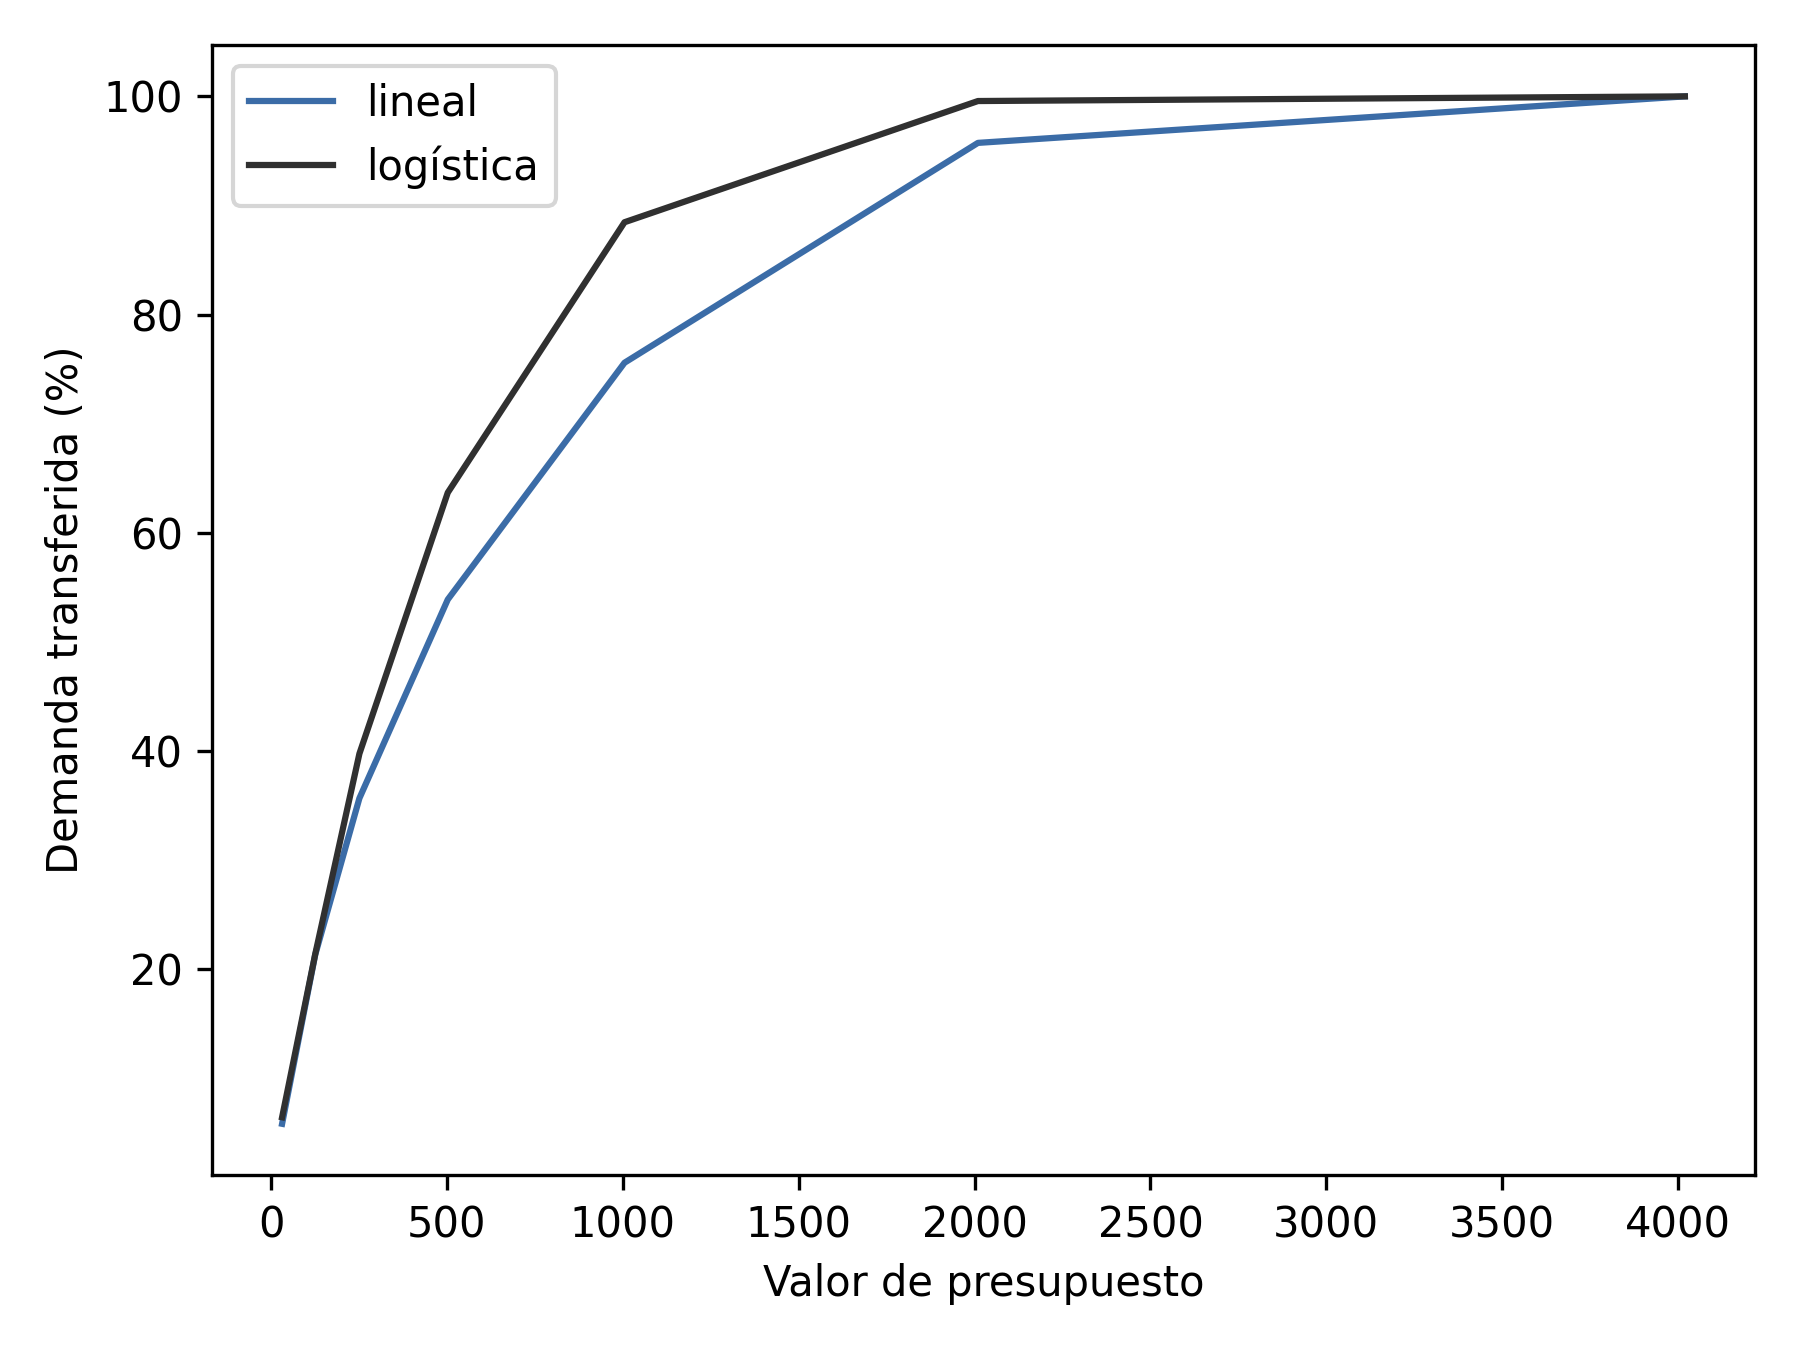
\includegraphics[width=8cm]{../resources/demand_by_budget.png}
    \caption{Porcentaje de demanda transferida total en función del presupuesto asignado para Sioux-Falls utilizando 20 puntos de quiebre y las funciones de transferencia de demanda lineal y logística. El comportamiento es similar en ambos casos y muestra que la eficiencia de aumentar el presupuesto no es siempre la misma.}
  \label{fig:demandtransferbybudgetlinear}
\end{figure}

Respecto a la utilización del presupuesto, vemos que a mayor presupuesto mayor es el porcentaje de gasto en los tipos de tecnologías más caras, lo cual es esperable dado que benefician más al usuario. Por otro lado, aumentar la cantidad de puntos de quiebre manteniendo presupuesto y función de transferencia fijas hace que el gasto en los tipos de tecnologías varíe, no necesariamente concentrando el gasto en los tipos más caros. El desglose del presupuesto utilizado por tecnología se detalla en la Tabla \ref{table:sensibilitybudgetusage} y en la Figura \ref{fig:sensibilitybudgetusage}.

Respecto a la complejidad de cada instancia y su relación con el tiempo de ejecución debemos notar que si bien hacemos referencia a esta relación en base a los resultados, entendemos que para sacar conclusiones al respecto deberíamos realizar un buen número de ejecuciones para cada instancia en lo que en CPLEX se llama modo oportunista, es decir paralelizar al máximo sin garantizar determinismo.

\begin{sidewaystable}
  \centering
  \small
  \begin{tabular}{cccccc}
      \toprule
      Instancia & Factor de presupuesto & \shortstack{Cantidad de puntos \\ de quiebre} & \shortstack{Función de \\ transferencia} & Demanda transferida (\%) & \shortstack{Tiempo ejecución \\ (hh:mm:ss)} \\
      \midrule
      1 & 0,1 & 5 & lineal & 4,65 & 00:00:02 \\
      2 & 0,1 & 20 & lineal & 5,81 & 00:00:11 \\
      3 & 0,1 & 5 & logística & 5,13 & 00:00:01 \\
      4 & 0,1 & 20 & logística & 6,41 & 00:00:08 \\
      5 & 0,4 & 5 & concavidad negativa & 32,43 & 00:00:36 \\
      6 & 0,4 & 20 & concavidad negativa & 36,49 & 00:07:40 \\
      7 & 0,4 & 50 & concavidad negativa & 37,39 & 00:07:29 \\
      8 & 0,4 & 5 & concavidad positiva & 15,50 & 00:00:18 \\
      9 & 0,4 & 20 & concavidad positiva & 17,05 & 00:09:38 \\
      10 & 0,4 & 50 & concavidad positiva & 18,22 & 14:07:09 \\
      11 & 0,4 & 5 & lineal & 18,60 & 00:00:24 \\
      12 & 0,4 & 20 & lineal & 21,32 & 00:06:17 \\
      13 & 0,4 & 50 & lineal & 22,09 & 00:31:55 \\
      14 & 0,4 & 5 & logística & 18,80 & 00:00:27 \\
      15 & 0,4 & 20 & logística & 21,37 & 00:12:35 \\
      16 & 0,4 & 50 & logística & 23,08 & 00:43:53 \\
      17 & 0,8 & 5 & lineal & 32,17 & 00:00:59 \\
      18 & 0,8 & 20 & lineal & 35,66 & 01:26:32 \\
      19 & 0,8 & 5 & logística & 35,47 & 00:00:44 \\
      20 & 0,8 & 20 & logística & 39,74 & 00:05:20 \\
      21 & 1,6 & 5 & lineal & 49,22 & 00:03:22 \\
      22 & 1,6 & 20 & lineal & 53,88 & 00:55:20 \\
      23 & 1,6 & 5 & logística & 58,97 & 00:02:36 \\
      24 & 1,6 & 20 & logística & 63,68 & 00:35:05 \\
      25 & 3,2 & 5 & lineal & 71,71 & 00:00:54 \\
      26 & 3,2 & 20 & lineal & 75,58 & 00:07:49 \\
      27 & 3,2 & 5 & logística & 80,77 & 00:01:33 \\
      28 & 3,2 & 20 & logística & 88,46 & 00:02:39 \\
      29 & 6,4 & 5 & lineal & 94,57 & 00:00:05 \\
      30 & 6,4 & 20 & lineal & 95,74 & 00:00:22 \\
      31 & 6,4 & 5 & logística & 97,44 & 00:00:02 \\
      32 & 6,4 & 20 & logística & 99,57 & 00:00:01 \\
      33 & 12,8 & 5 & lineal & 100,00 & 00:00:00 \\
      34 & 12,8 & 20 & lineal & 100,00 & 00:00:00 \\
      35 & 12,8 & 5 & logística & 100,00 & 00:00:00 \\
      36 & 12,8 & 20 & logística & 100,00 & 00:00:00 \\
      \bottomrule
  \end{tabular}
  \caption{Todas las instancias fueron solucionadas al óptimo en tiempos relativamente cortos, con excepción de dos instancias cuyo tiempo de ejecución fue más de una hora.} \label{table:sensibilityresults}
\end{sidewaystable}

\begin{sidewaystable}
  \centering
  \small
  \begin{tabular}{cccccccc}
      \toprule
      Instancia & Presupuesto & Presupuesto utilizado & Tecn. 1 (\%) & Tecn. 2 (\%) & Tecn. 3 (\%) & Tecn. 4 (\%) & Tecn. 5 (\%) \\
      \midrule
      1 & 31.4 & 31 & 35.48 & 64.52 &  &  &  \\
      2 & 31.4 & 31 & 9.68 & 90.32 &  &  &  \\
      3 & 31.4 & 30 &  & 46.67 & 53.33 &  &  \\
      4 & 31.4 & 31 & 9.68 & 51.61 & 38.71 &  &  \\
      5 & 125.6 & 125 & 10.4 & 83.2 & 6.4 &  &  \\
      6 & 125.6 & 125 & 4.0 & 89.6 & 6.4 &  &  \\
      7 & 125.6 & 125 & 5.6 & 81.6 & 12.8 &  &  \\
      8 & 125.6 & 125 & 2.4 & 24.0 & 41.6 & 32.0 &  \\
      9 & 125.6 & 125 & 7.2 & 12.8 & 48.0 & 32.0 &  \\
      10 & 125.6 & 125 & 2.4 & 27.2 & 51.2 & 19.2 &  \\
      11 & 125.6 & 125 & 15.2 & 33.6 & 51.2 &  &  \\
      12 & 125.6 & 125 & 16.8 & 70.4 & 12.8 &  &  \\
      13 & 125.6 & 125 & 5.6 & 81.6 & 12.8 &  &  \\
      14 & 125.6 & 125 & 4.0 & 44.8 & 38.4 & 12.8 &  \\
      15 & 125.6 & 125 & 5.6 & 11.2 & 70.4 & 12.8 &  \\
      16 & 125.6 & 125 & 2.4 & 36.8 & 60.8 &  &  \\
      17 & 251.2 & 251 & 5.18 & 35.86 & 36.65 & 22.31 &  \\
      18 & 251.2 & 251 & 8.37 & 21.51 & 70.12 &  &  \\
      19 & 251.2 & 251 & 1.99 & 21.51 & 44.62 & 31.87 &  \\
      20 & 251.2 & 251 & 1.2 & 11.16 & 81.27 & 6.37 &  \\
      21 & 502.4 & 502 & 0.4 & 15.94 & 19.92 & 63.75 &  \\
      22 & 502.4 & 502 & 2.39 & 7.57 & 45.42 & 44.62 &  \\
      23 & 502.4 & 501 & 2.2 & 13.97 & 35.93 & 47.9 &  \\
      24 & 502.4 & 502 & 2.79 & 5.58 & 54.98 & 36.65 &  \\
      25 & 1004.8 & 1002 & 0.4 & 4.19 & 13.17 & 19.96 & 62.28 \\
      26 & 1004.8 & 1004 &  & 5.98 & 6.37 & 49.4 & 38.25 \\
      27 & 1004.8 & 1004 & 0.6 & 2.99 & 26.29 & 17.53 & 52.59 \\
      28 & 1004.8 & 1004 & 0.8 & 1.2 & 14.34 & 83.67 &  \\
      29 & 2009.6 & 2008 &  & 0.4 & 4.38 & 3.59 & 91.63 \\
      30 & 2009.6 & 2008 &  & 0.4 & 1.59 & 10.36 & 87.65 \\
      31 & 2009.6 & 2008 & 0.1 & 1.49 & 2.39 & 1.99 & 94.02 \\
      32 & 2009.6 & 2004 &  & 0.6 & 1.6 & 14.77 & 83.03 \\
      33 & 4019.2 & 2719 & 0.26 & 0.29 & 1.18 &  & 98.27 \\
      34 & 4019.2 & 3048 &  & 0.26 &  &  & 99.74 \\
      35 & 4019.2 & 2780 & 0.14 & 0.86 &  &  & 98.99 \\
      36 & 4019.2 & 2994 & 0.07 &  & 0.53 &  & 99.4 \\
      \bottomrule
  \end{tabular}
  \caption{Detalle de presupuesto utilizado por instancia por tipo de tecnología. Las columnas Presupuesto y Presupuesto Utilizado están en unidades de presupuesto. Los porcentajes se calcularon sobre el valor de presupuesto utilizado y pueden no sumar 100\% por el redondeo realizado.} \label{table:sensibilitybudgetusage}
\end{sidewaystable}

\begin{figure}[h!]
  \centering
  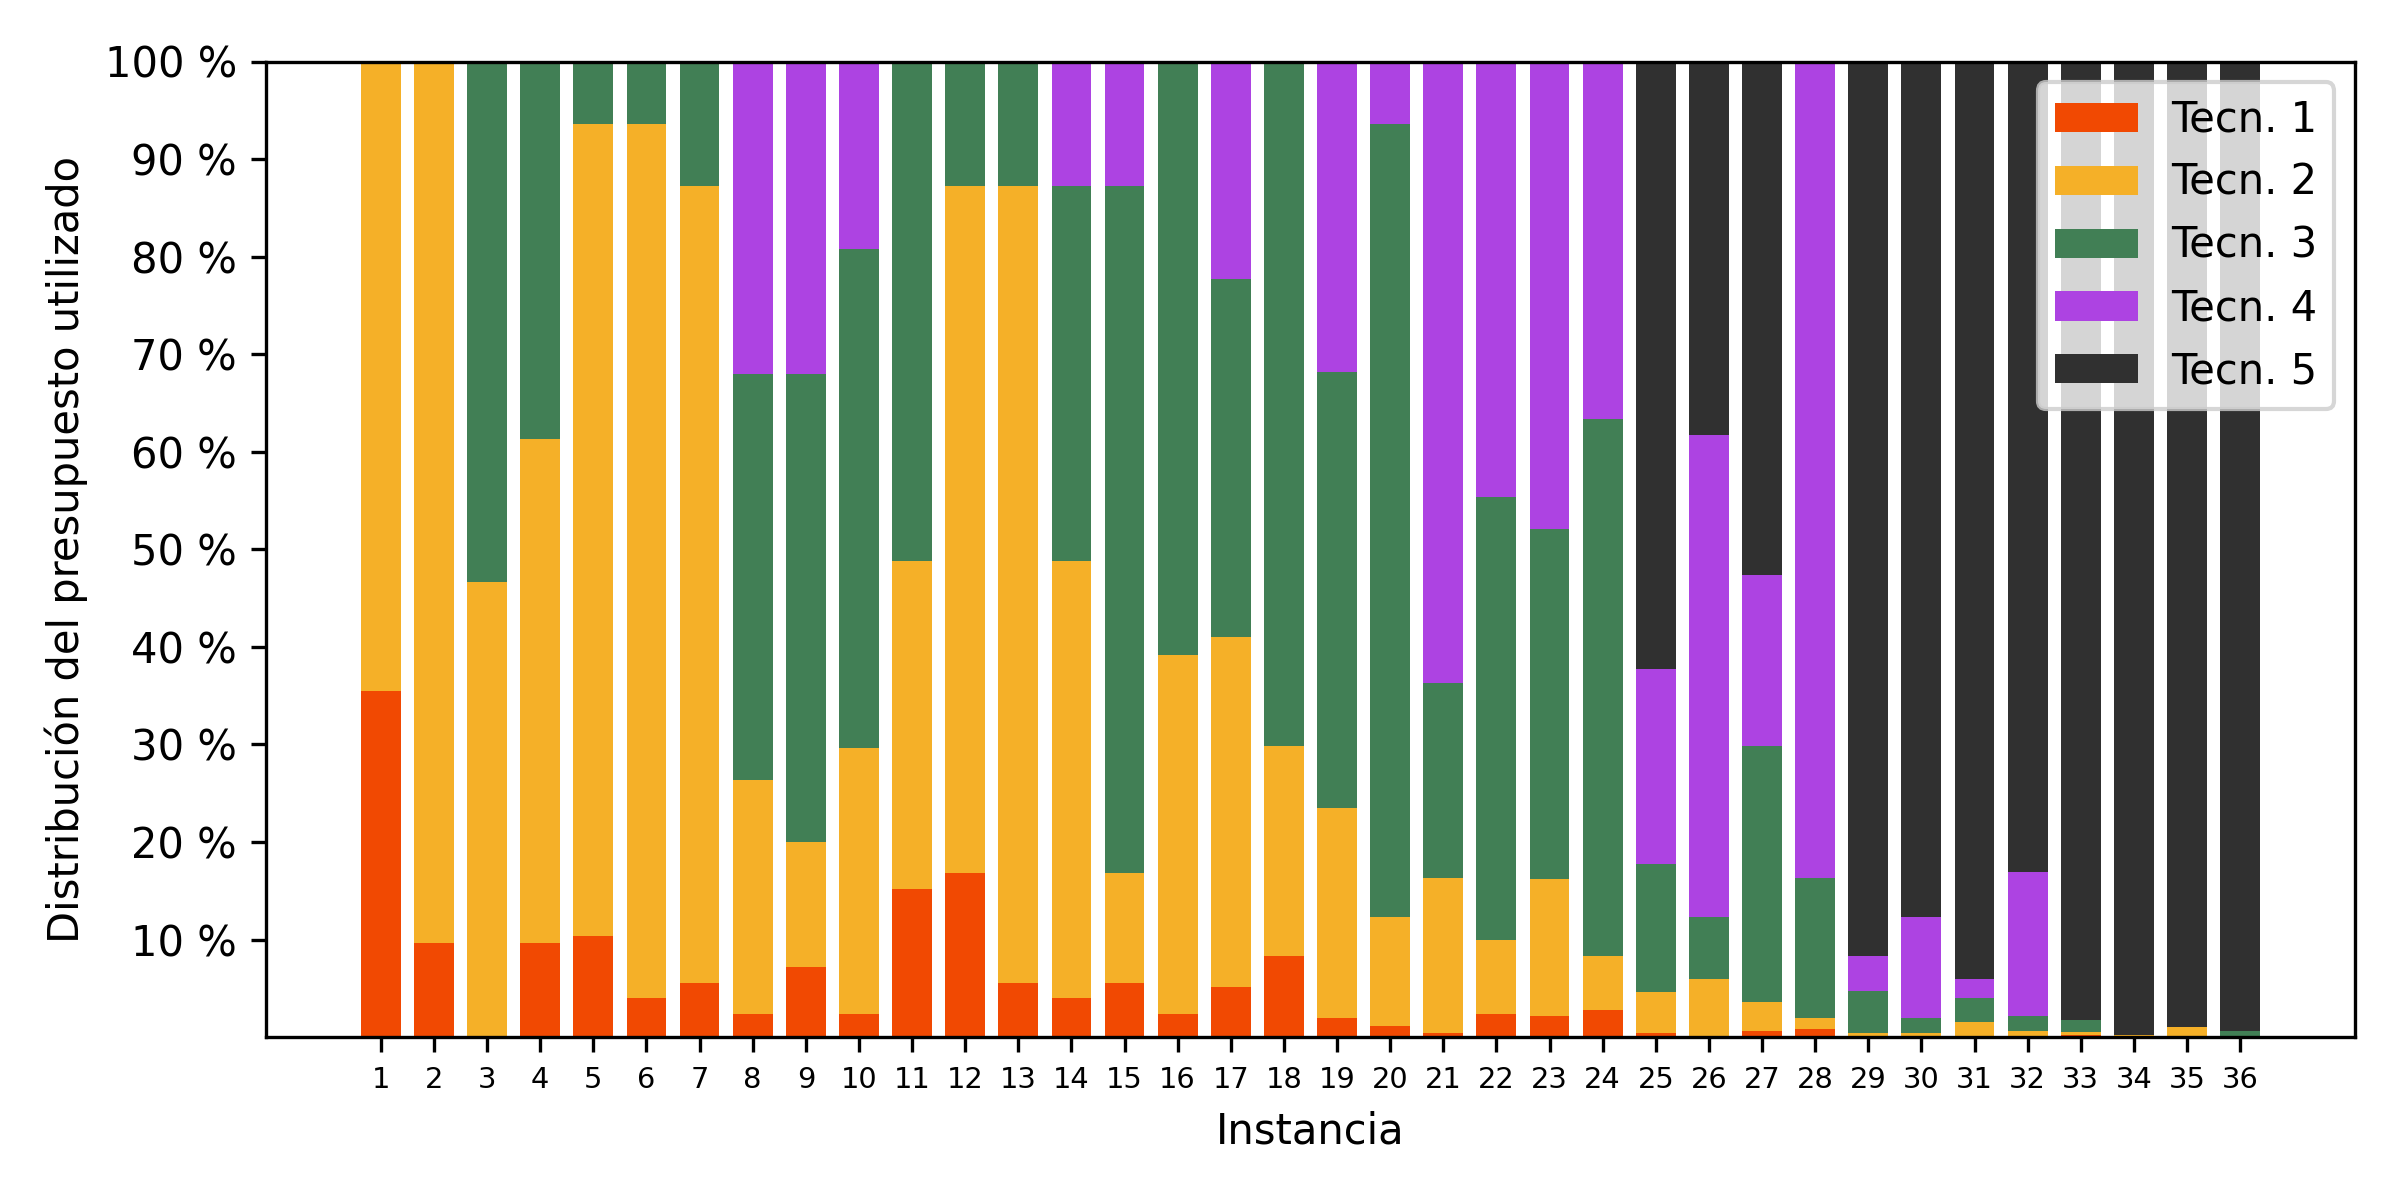
\includegraphics[width=14cm]{../resources/budget_use_by_infra.png}
  \caption{Visualización de la distribución del uso del presupuesto para cada instancia.}
  \label{fig:sensibilitybudgetusage}
\end{figure}

\begin{figure}[h!]
  \centering
  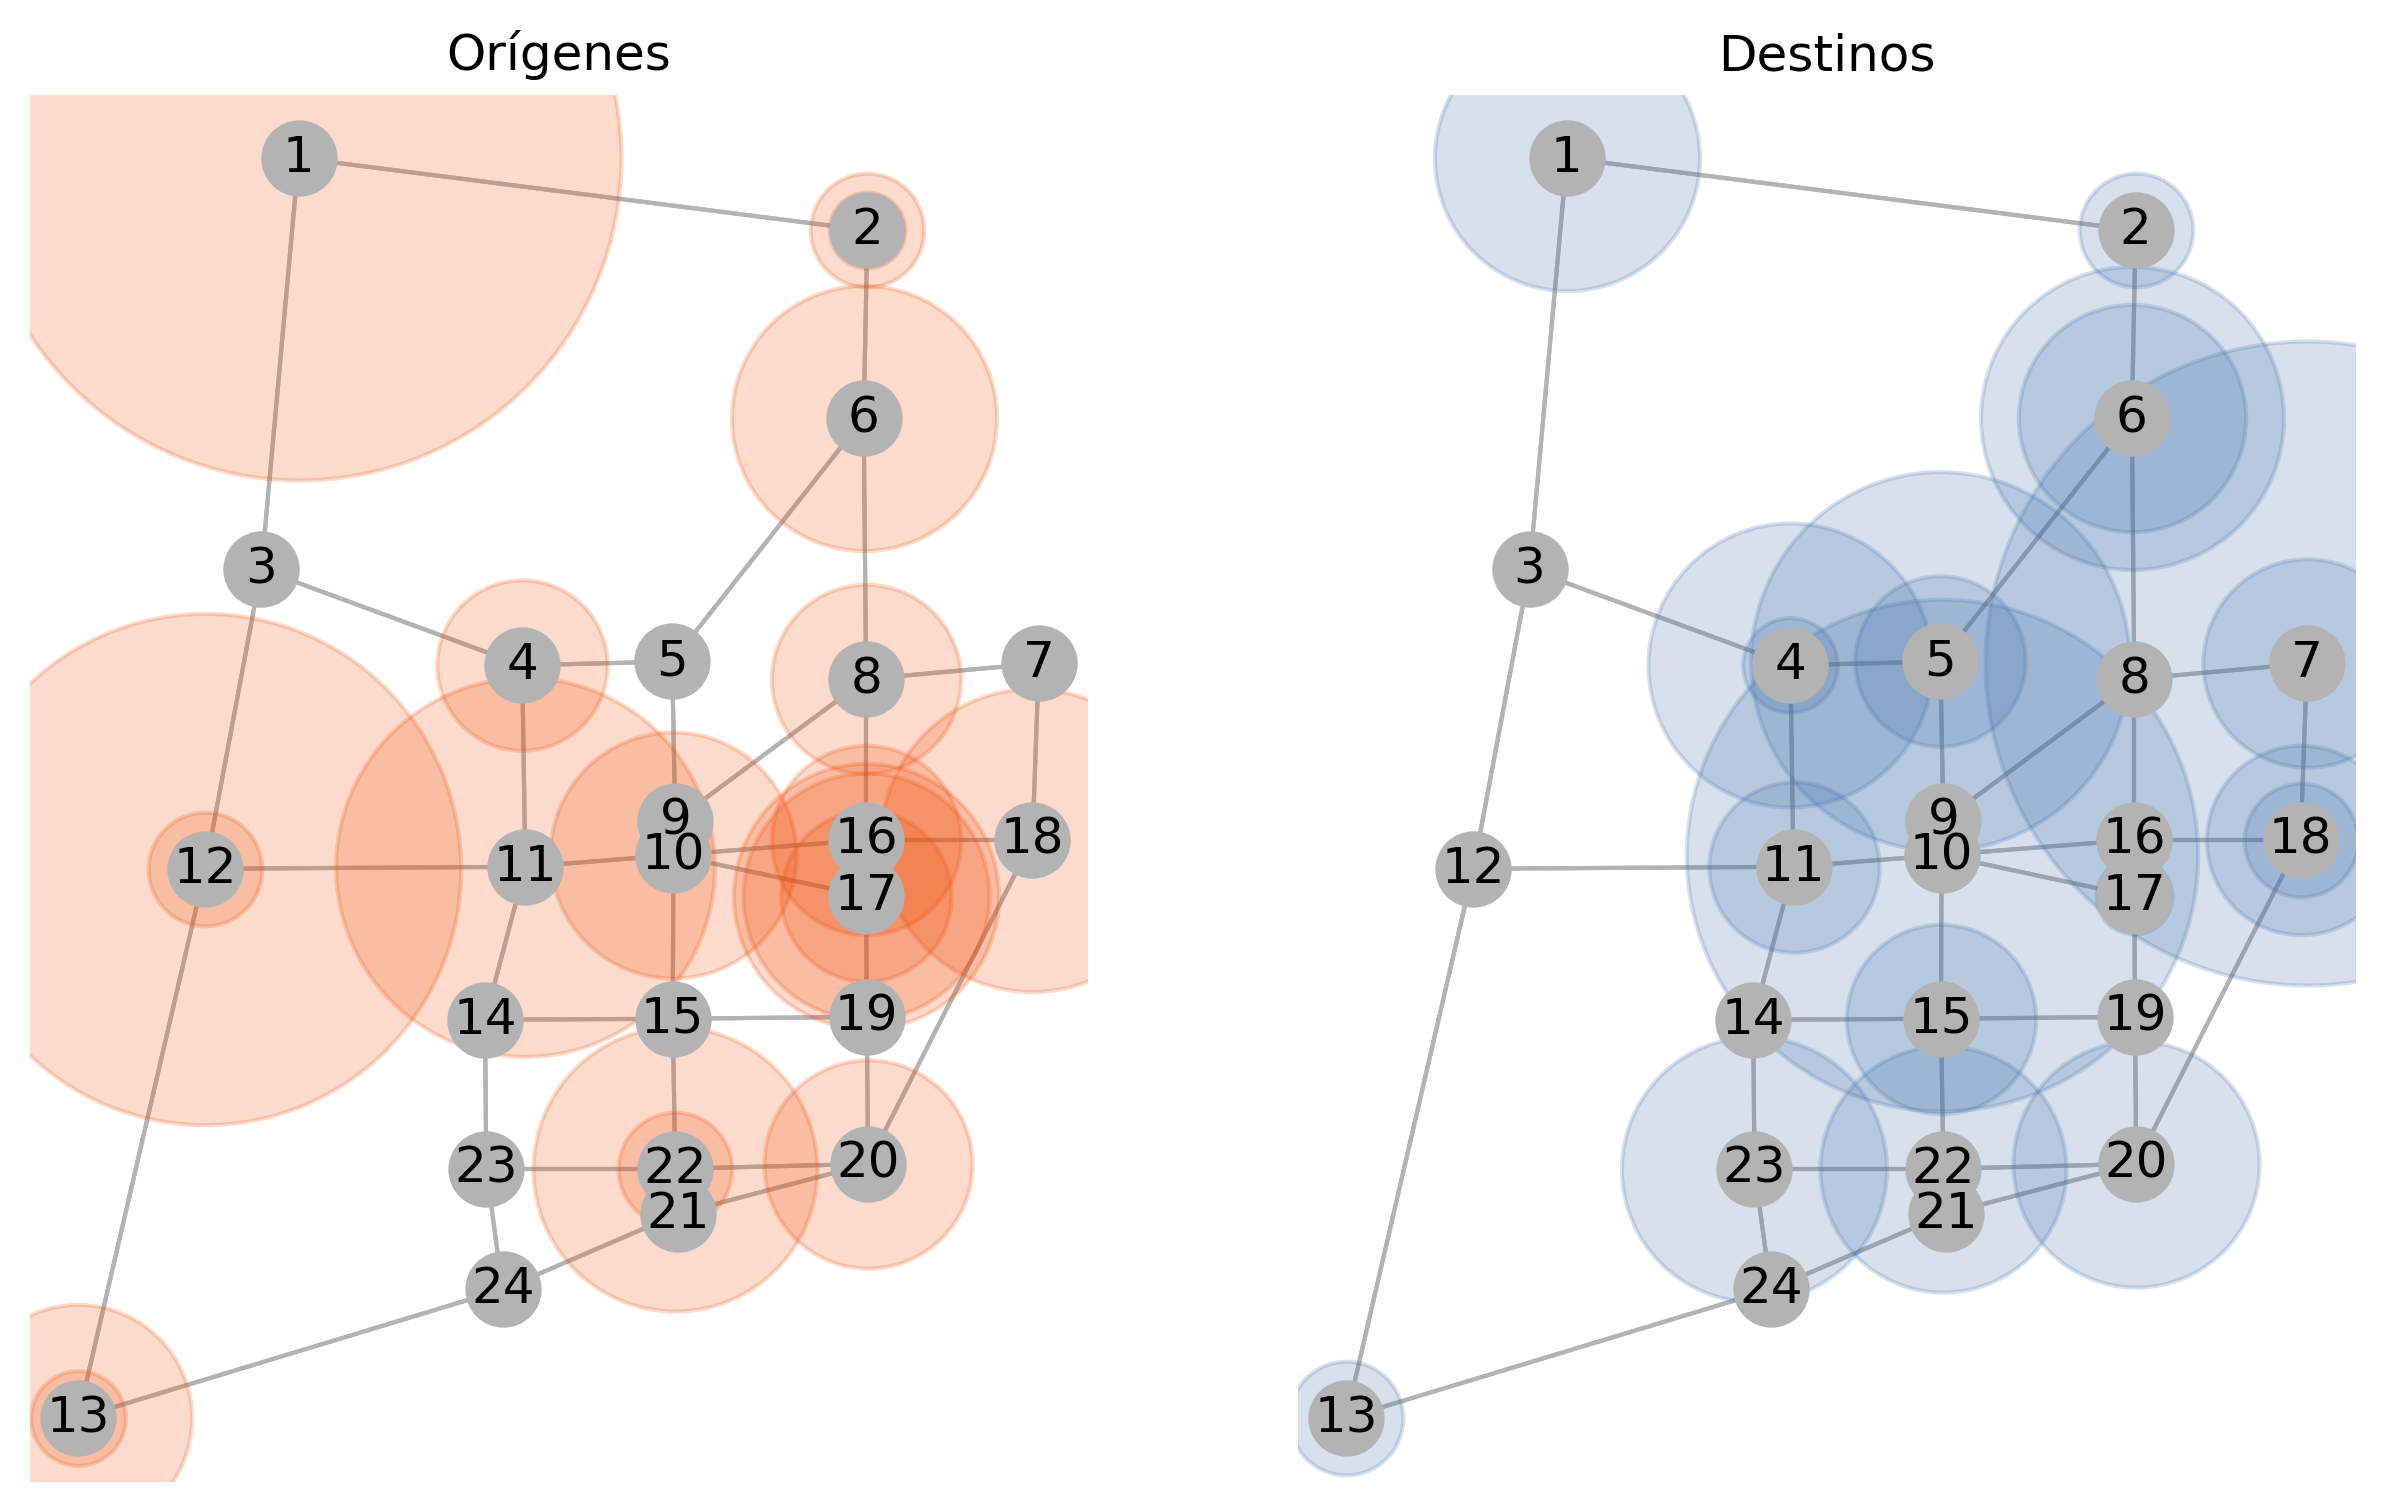
\includegraphics[width=12cm]{../resources/sioux_falls_demand.png}
  \caption{Visualización de la distribución de nodos origen y destino junto a su valor de demanda representado por el tamaño de los círculos para la instancia de Sioux-Falls. A la izquierda se ubican los orígenes y a la derecha los destinos. Los tamaños de los círculos son proporcionales al valor de demanda y no se suman por nodo.}
  \label{fig:sioux_falls_demand}
\end{figure}

\clearpage
\subsection*{Casos particulares}

Vamos a analizar en detalle algunos casos particulares y discutir cómo afecta la cantidad de puntos de quiebre a la decisiones de cuales tecnologías construir. Comparamos las instancias 11, 12 y 13, que utilizan la función lineal de transferencia de demanda con 5, 20 y 50 puntos de quiebre respectivamente y un factor de presupuesto de 40\%. Más datos específicos de cada instancia se pueden apreciar en la Tabla \ref{table:sensibilityinfralengths} y Figura \ref{fig:sensibilityinstance11_12_13}. Observamos que a mayor cantidad de puntos de quiebre más inteligentes son las decisiones tomadas. Por ejemplo, en la instancia 11 la mitad del acotado presupuesto se invirtió en poco cubrimiento de calles utilizando la tecnología 3 mientras que en la 12 y 13 el gasto en esta tecnología sólo fue el 12\%. En las instancias 12 y 13 la mayor parte del gasto se hizo en tecnología 2 que para el nivel de presupuesto y función de transferencia de demanda parece ser la más eficiente. En particular, los datos de porcentaje del largo total de las calles cubierto desglosado por tipo de tecnología nos da una idea general de la demanda afectada, al ser esta instancia altamente densa y uniforme en términos de orígenes y destinos, como se observa en la Figura \ref{fig:sioux_falls_demand}.

 \begin{table}[h!]
  \centering
  \begin{tabular}{ccccc}
    \toprule
      Instancia & Tecn. 1 (\%) & Tecn. 2 (\%) & Tecn. 3 (\%) & Total (\%) \\
    \midrule
      11 & 8,74  & 6,51   & 5,72 & 20,98 \\
      12 & 8,89  & 15,22  & 1,64 & 25,75 \\
      13 & 2,29  & 17,77  & 1,96 & 22,73 \\
    \bottomrule
  \end{tabular}
  \caption{Porcentaje del largo total de arcos de la red construido con cada tipo de tecnología (excluyendo la tecnología base) para las instancias de interés.}\label{table:sensibilityinfralengths}
\end{table}

Si observamos los datos de demanda transferida y costo de camino más corto, Figura \ref{fig:sensibilitybyodpair_11_12_13}, vemos que a mayor cantidad de puntos de quiebre mayor es la cantidad de pares origen-destino afectada aunque en general las decisiones de cuáles pares origen-destino y cuánto mejorarlos no fue muy diferente entre instancias.

\begin{figure}[h!]
  \centering
  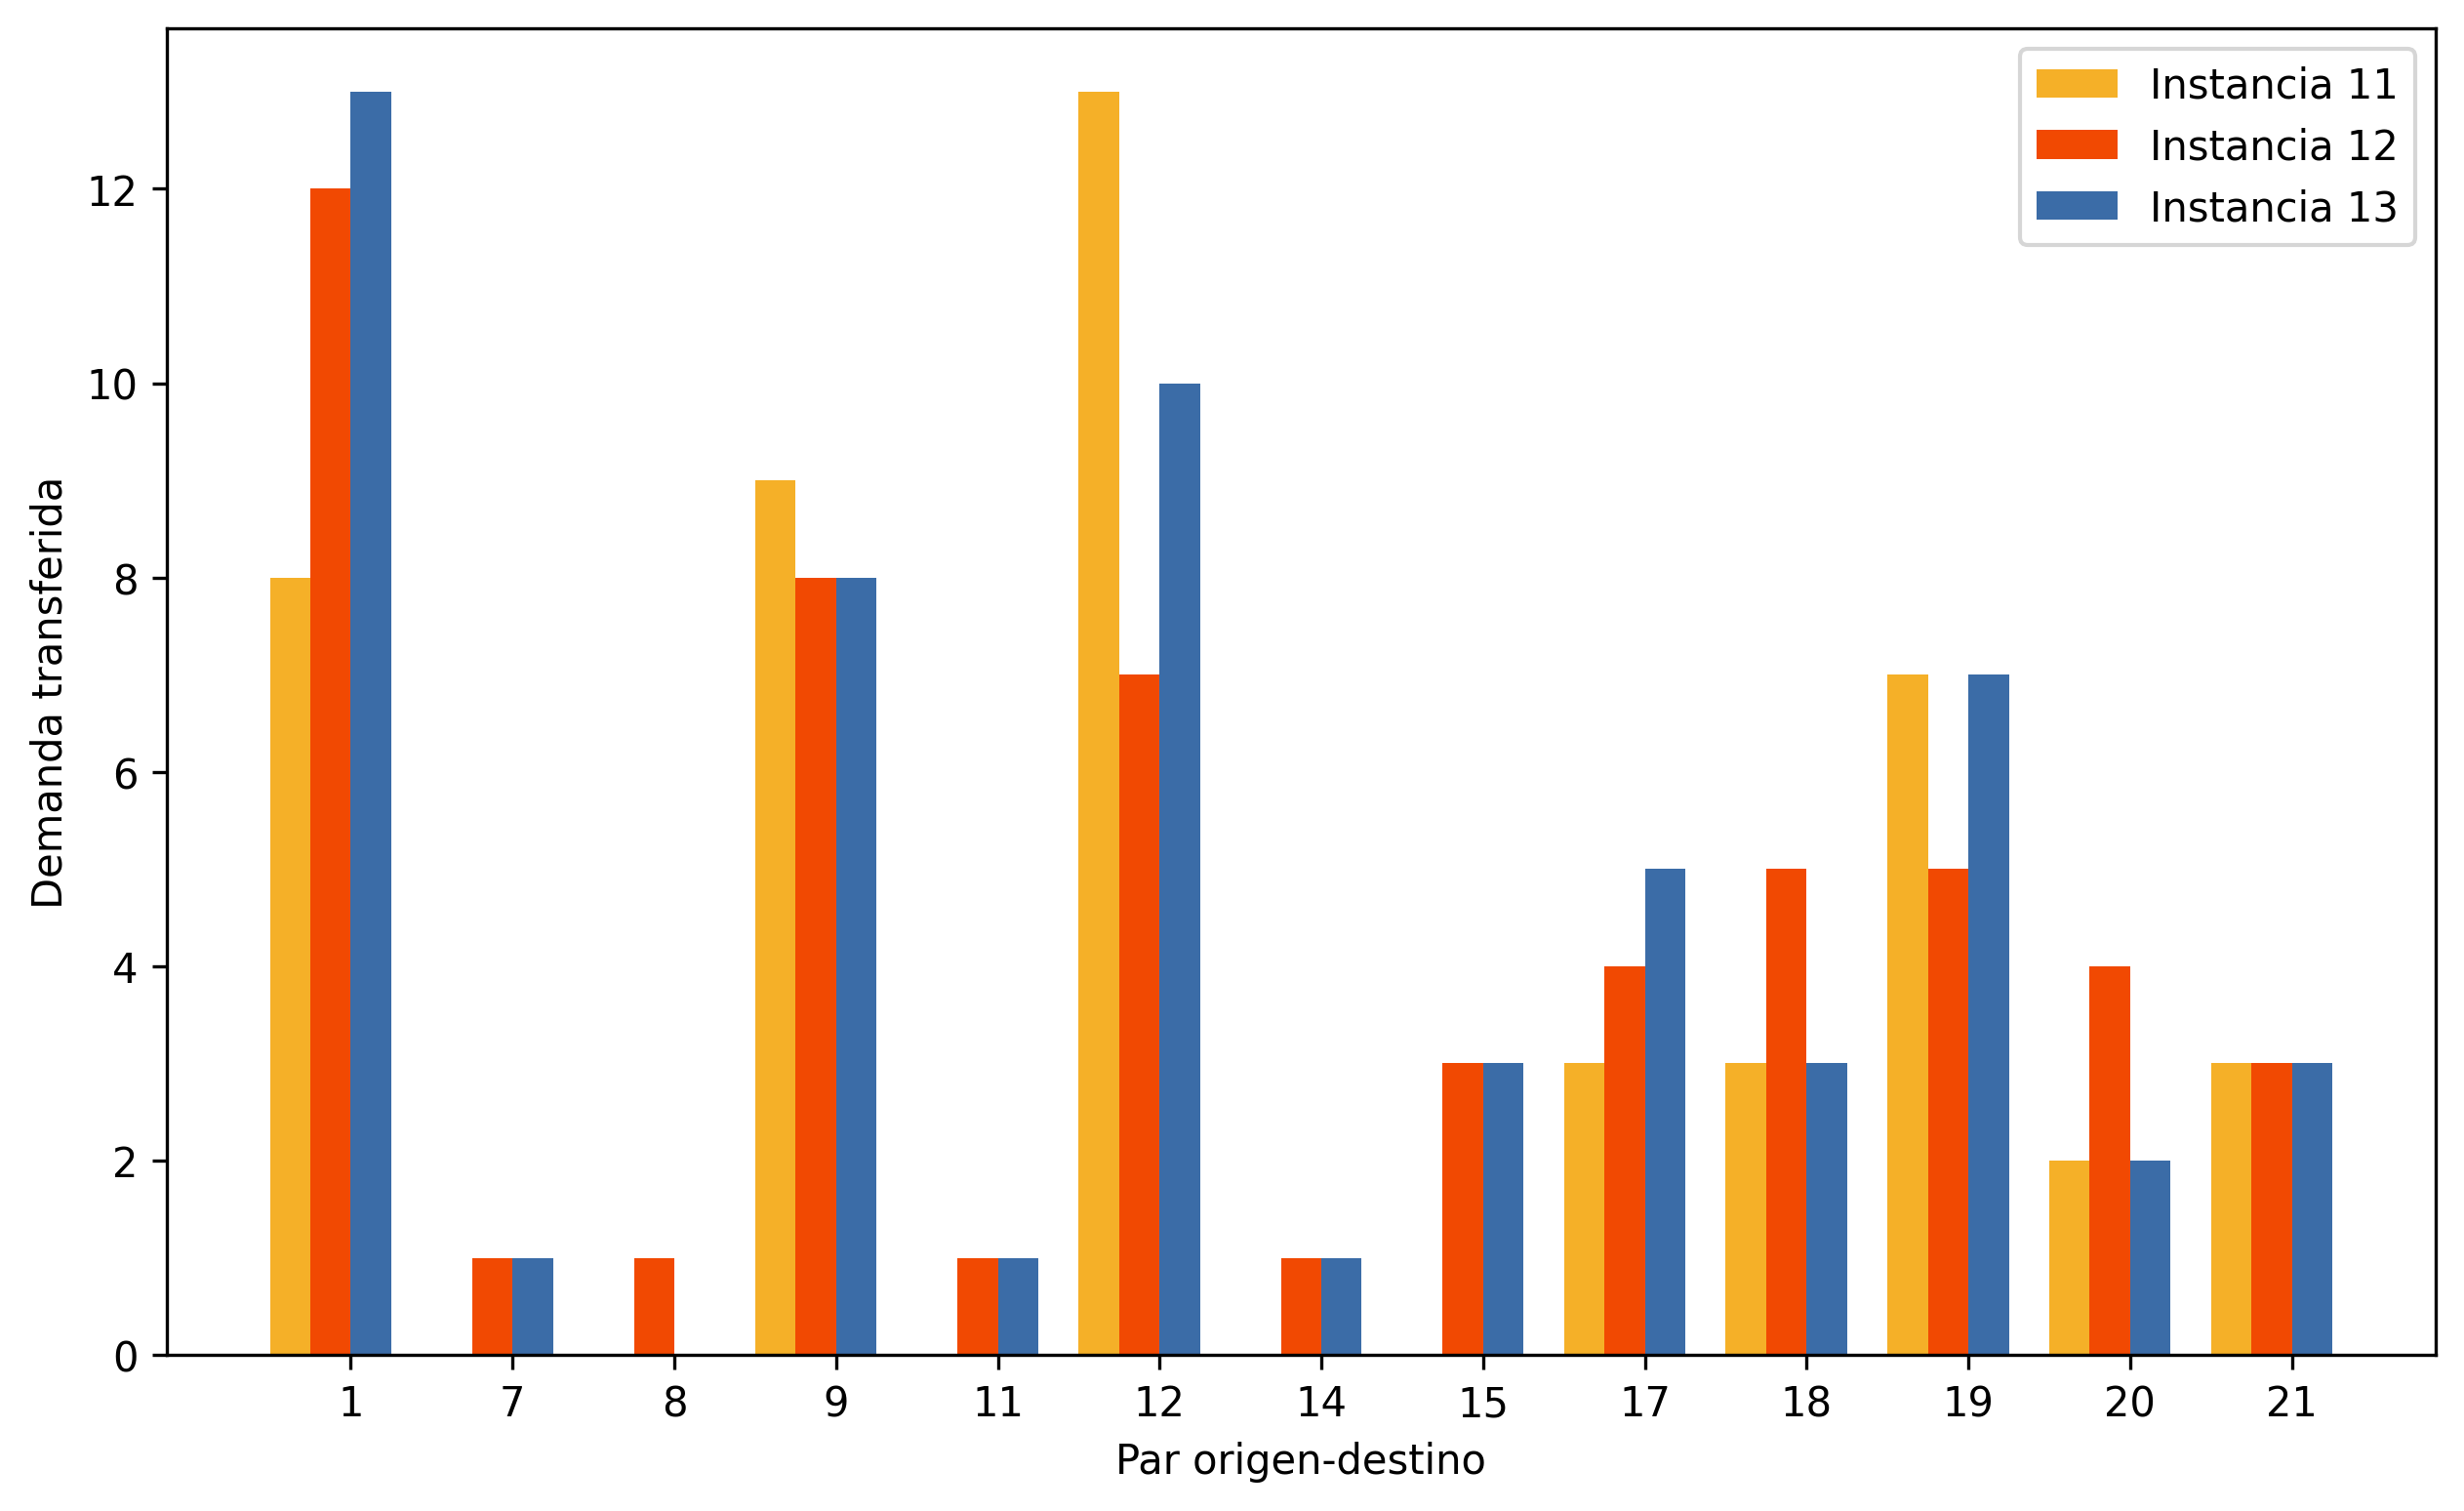
\includegraphics[width=12cm]{../resources/sensibility_case_study_demand.png}
  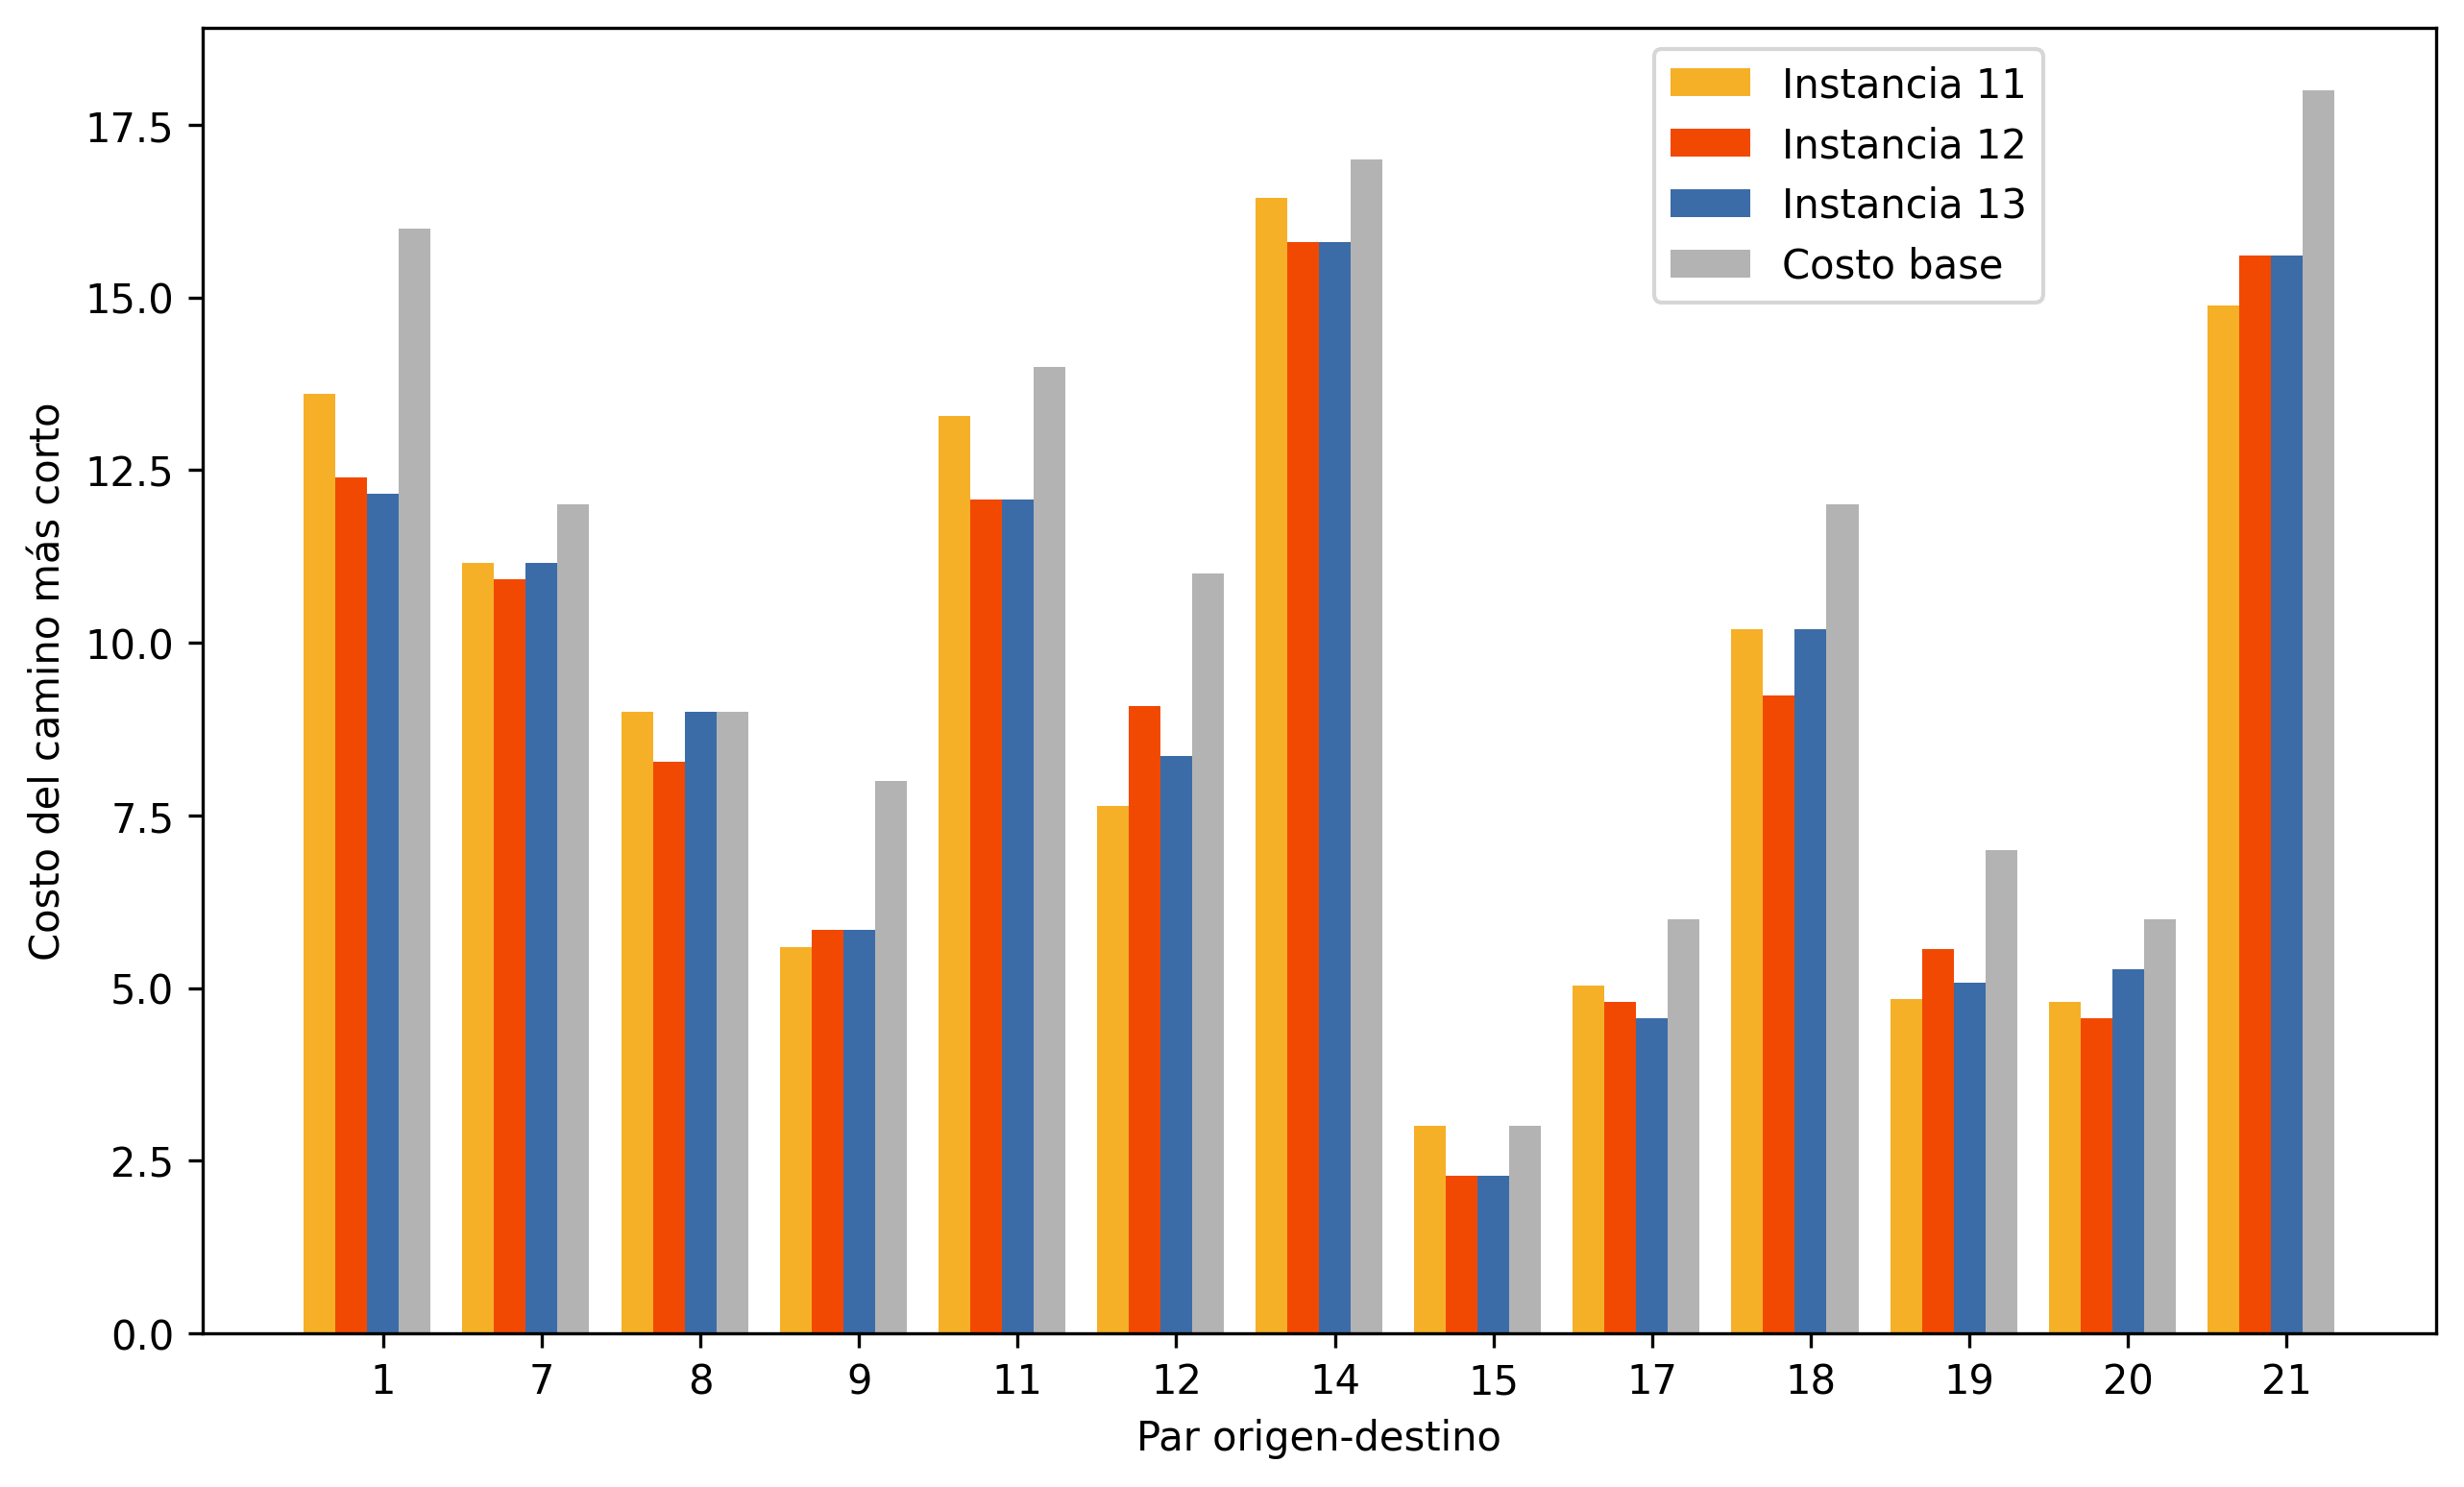
\includegraphics[width=12cm]{../resources/sensibility_case_study_shortest_paths.png}
  \caption{Demanda transferida y costo del camino más corto para los pares origen-destino para los cuales hubo demanda transferida. Los pares origen-destino se numeran de acuerdo a la Tabla \ref{table:siouxfallsdemanddata} en el Apéndice \ref{sect:siouxfallsdata}. Los costos de los caminos más cortos se comparan contra el costo base que es aquel sobre la red en la cual no hay infraestructura de ciclovía construida.}
  \label{fig:sensibilitybyodpair_11_12_13}
\end{figure}

\begin{figure}[h!]
  \centering
  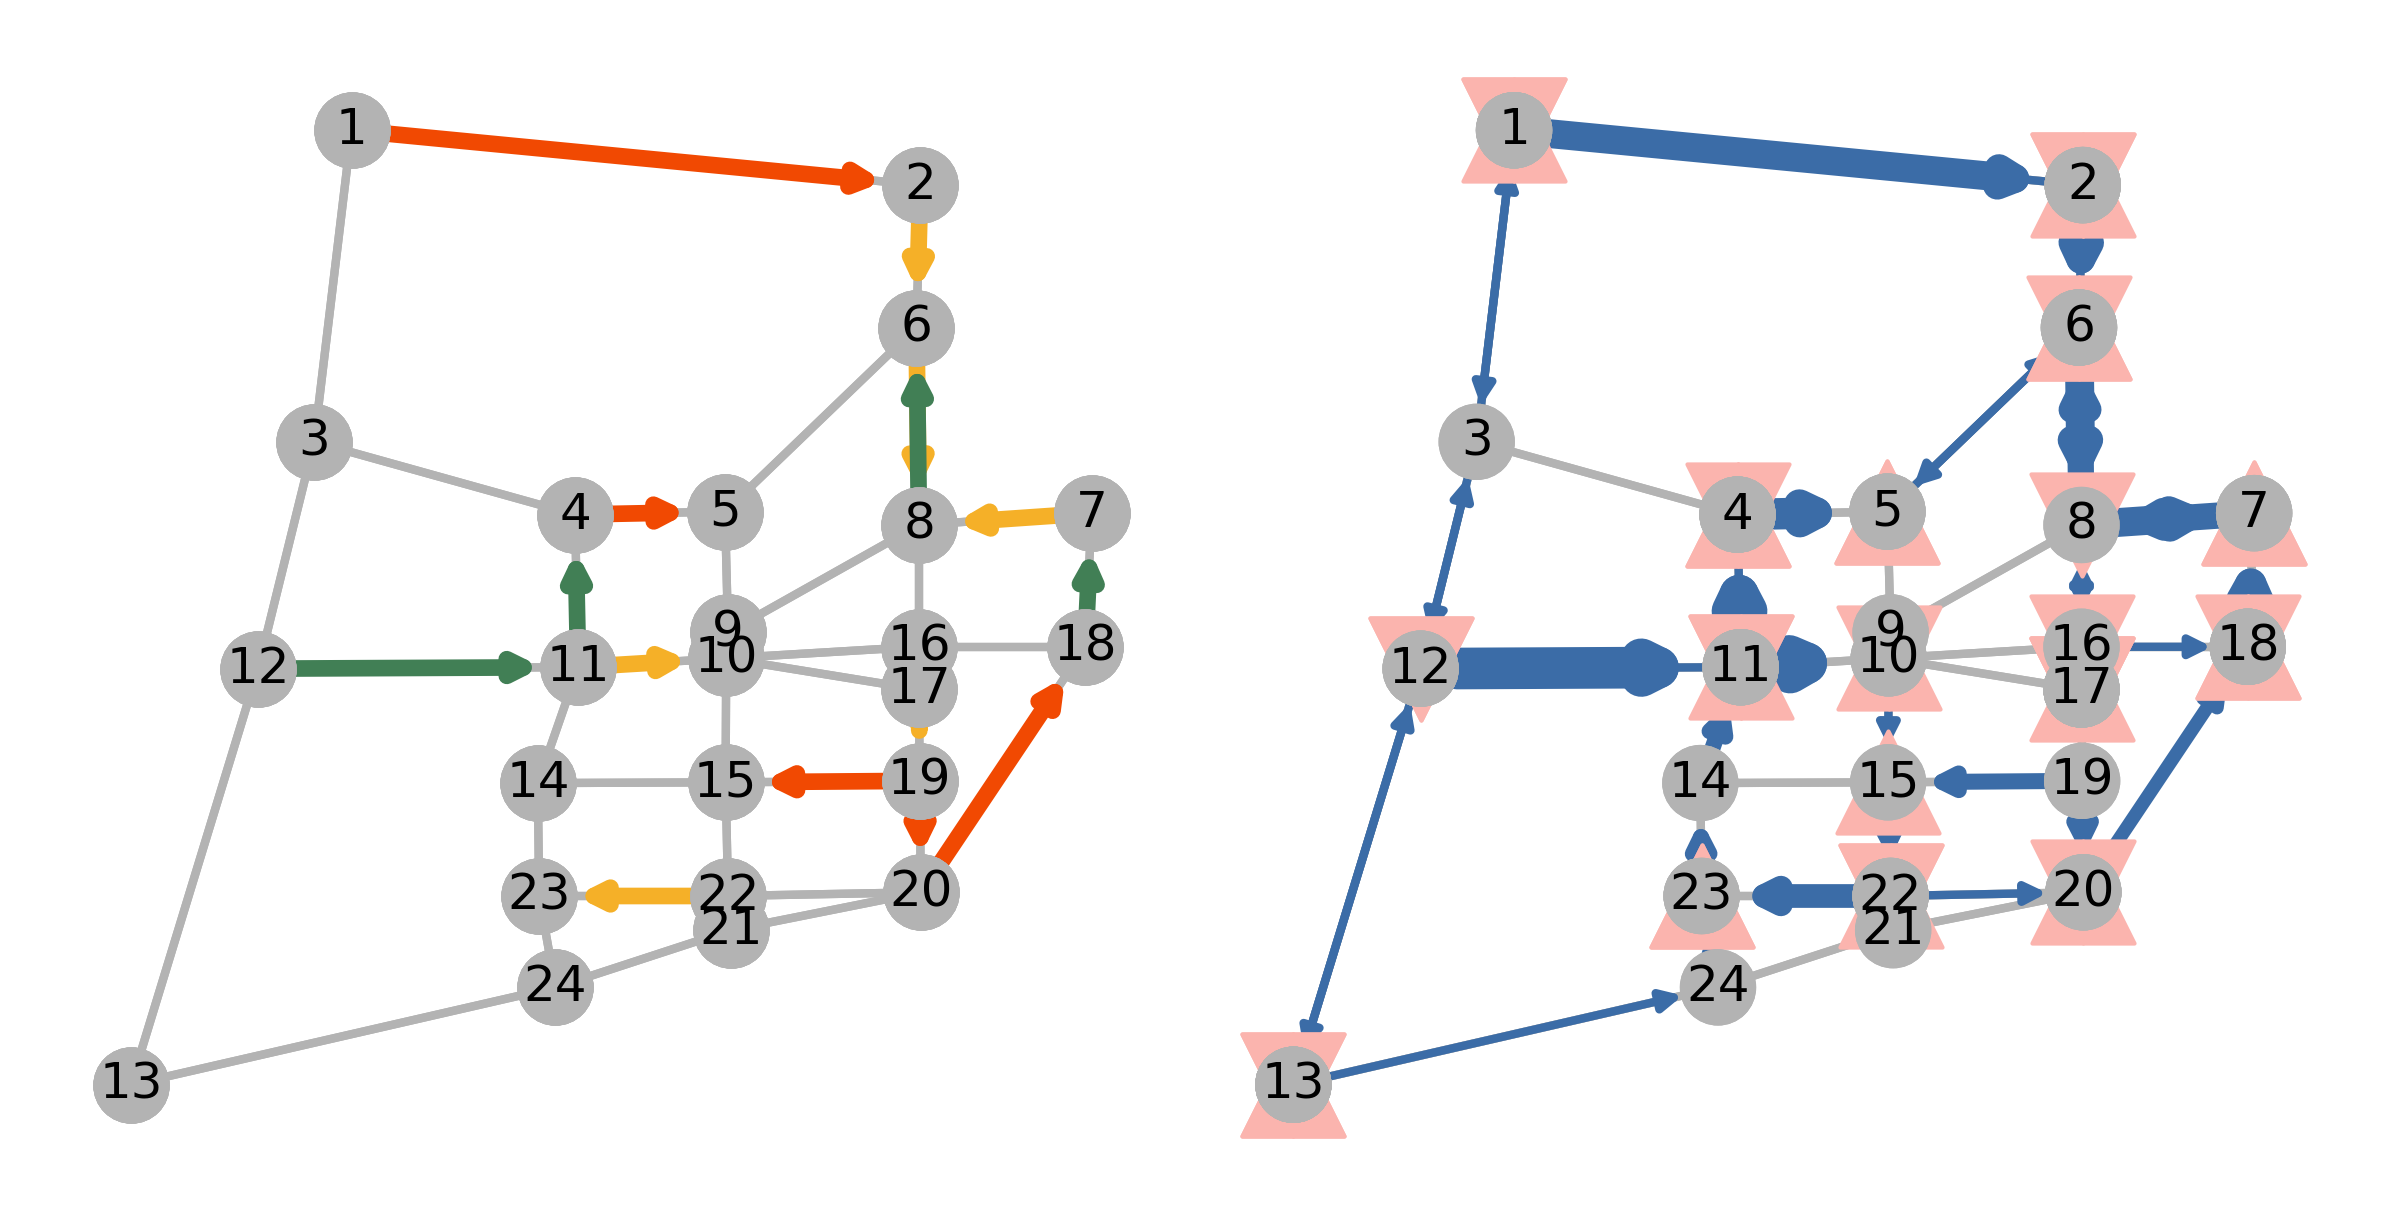
\includegraphics[width=10cm]{../resources/sioux_falls_0.4_budget_factor_linear_5_breakpoints.png}
  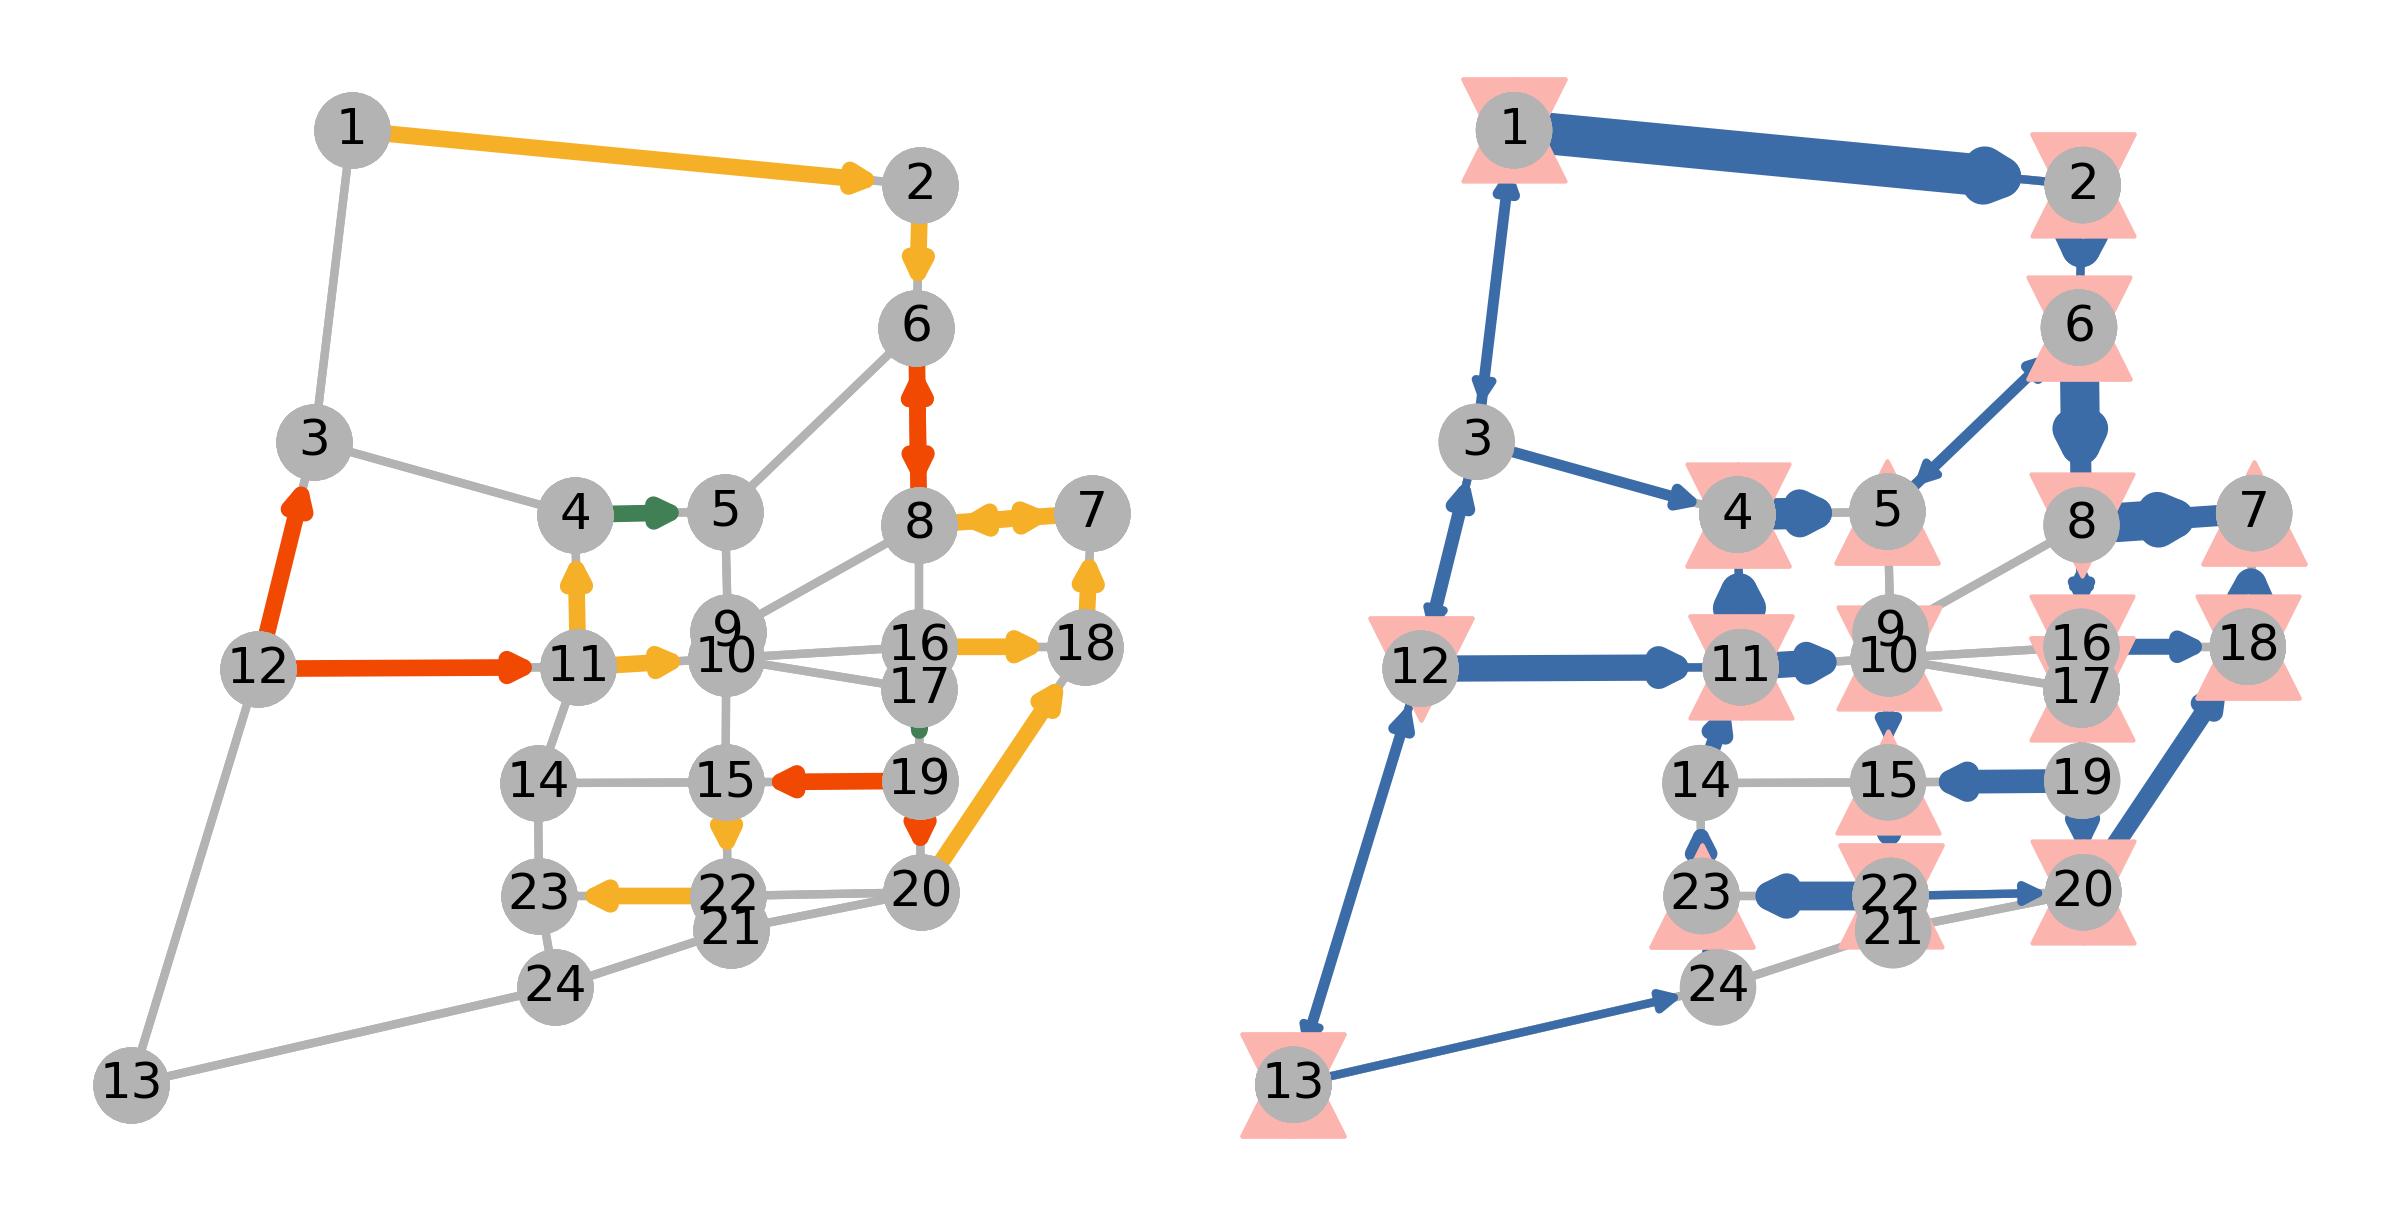
\includegraphics[width=10cm]{../resources/sioux_falls_0.4_budget_factor_linear_20_breakpoints.png}
  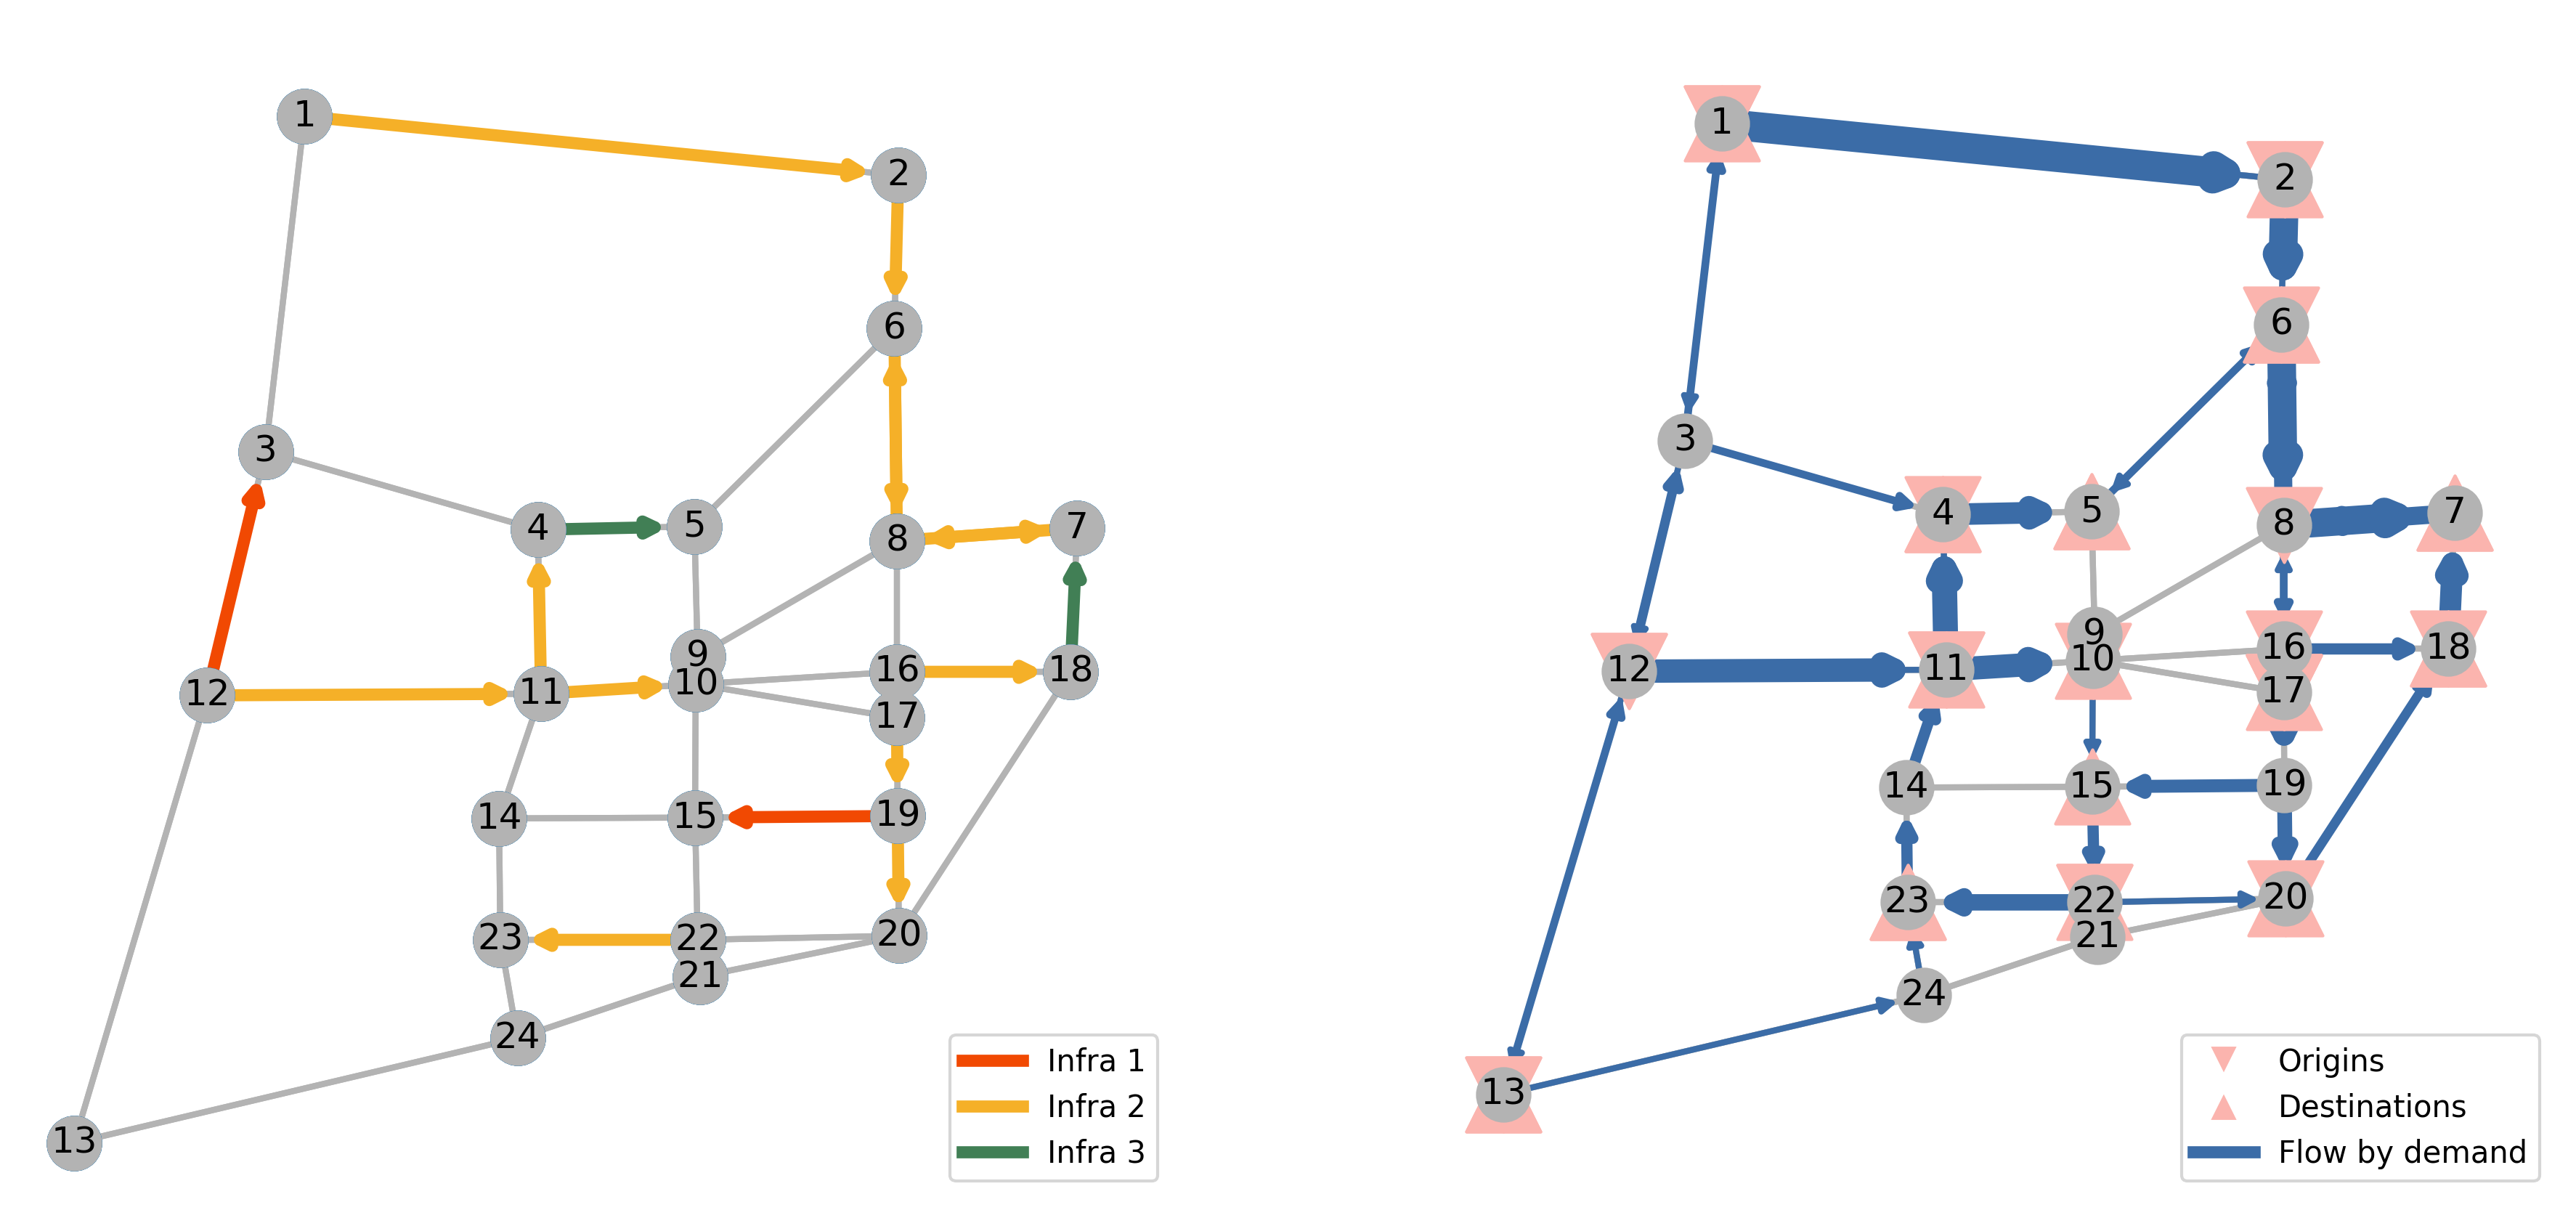
\includegraphics[width=10cm]{../resources/sioux_falls_0.4_budget_factor_linear_50_breakpoints.png}
  \caption{De arriba hacia abajo, instancia 11, 12 y 13. A la izquierda se muestran las ubicaciones de cada tipo de tecnología. A la derecha los flujos para cada arco considerando el acumulado de demanda de cada par origen-destino que pasaría sobre ellos. Los flujos no se agregan entre dos arcos adyacentes con sentido opuesto, en dicho caso solo se visualiza el mayor de los flujos.}
  \label{fig:sensibilityinstance11_12_13}
\end{figure}

\FloatBarrier
\section{Aplicación a un caso real}

Utilizamos una instancia de la ciudad de Montevideo de manera de poder analizar la aplicación práctica del problema sobre datos familiares y realistas. Los datos de la instancia provienen de una red sobre una zonificación de la ciudad que resulta en un grafo de 136 nodos y 636 arcos. Respecto a la demanda, consideramos los 600 pares origen-destino de mayor demanda que cumplen que el origen y destino no se encuentran a más de 3 km de distancia euclídea entre ellos. Encontramos que una distancia 3 km en línea recta, que implica una distancia Manhattan máxima de poco más de 4.2 km, es un límite razonable para viajes en bicicleta común y eléctricas según \cite{anette2018}, donde se estima una distancia de viaje promedio de 2.6 km y 3 km respectivamente. Además, está dentro de lo que \cite{shwe2014} considera un viaje potencial en bicicleta, es decir, menor a 5 km.

\subsection{Descripción de la instancia}

La ciudad de Montevideo es de mayor tamaño en el Uruguay. Incluyendo el área metropolitana cuenta con una población de cerca de 1.8 millones de personas y una densidad de población de 6726 habitantes por $km^2$. La ciudad cuenta con un sistema de transporte de autobuses que, junto al transporte privado automotor, abarcan la mayor parte de la demanda de viajes \cite{Mauttone2017a}.

La instancia utilizada corresponde a una simplifición de la red de calles de la ciudad, observar la comparación en la Figura \ref{fig:montevideosimplification}. La red simplificada fue desarrollada dentro de un proyecto de la Comisión Sectorial de Investigación Científica, CSIC \footnote{\url{https://www.csic.edu.uy/}}, y consiste en una zonificación de la ciudad donde los nodos corresponden a los centroides de cada zona y los arcos modelan la adyacencia entre zonas. Por otro lado, la matriz de demanda se tomó del \cite{Massobrio2020}, en donde se realiza un estudio y relevamiento de la demanda de viajes de la ciudad a partir de datos de uso del sistema transporte público de pasajeros en la ciudad de Montevideo. Si bien los datos de demandas no son específicos del transporte en bicicleta, los utilizamos por ser uno de los conjuntos de datos de viajes más complejos que hay disponibles.

\begin{figure}[h!]
  \centering
  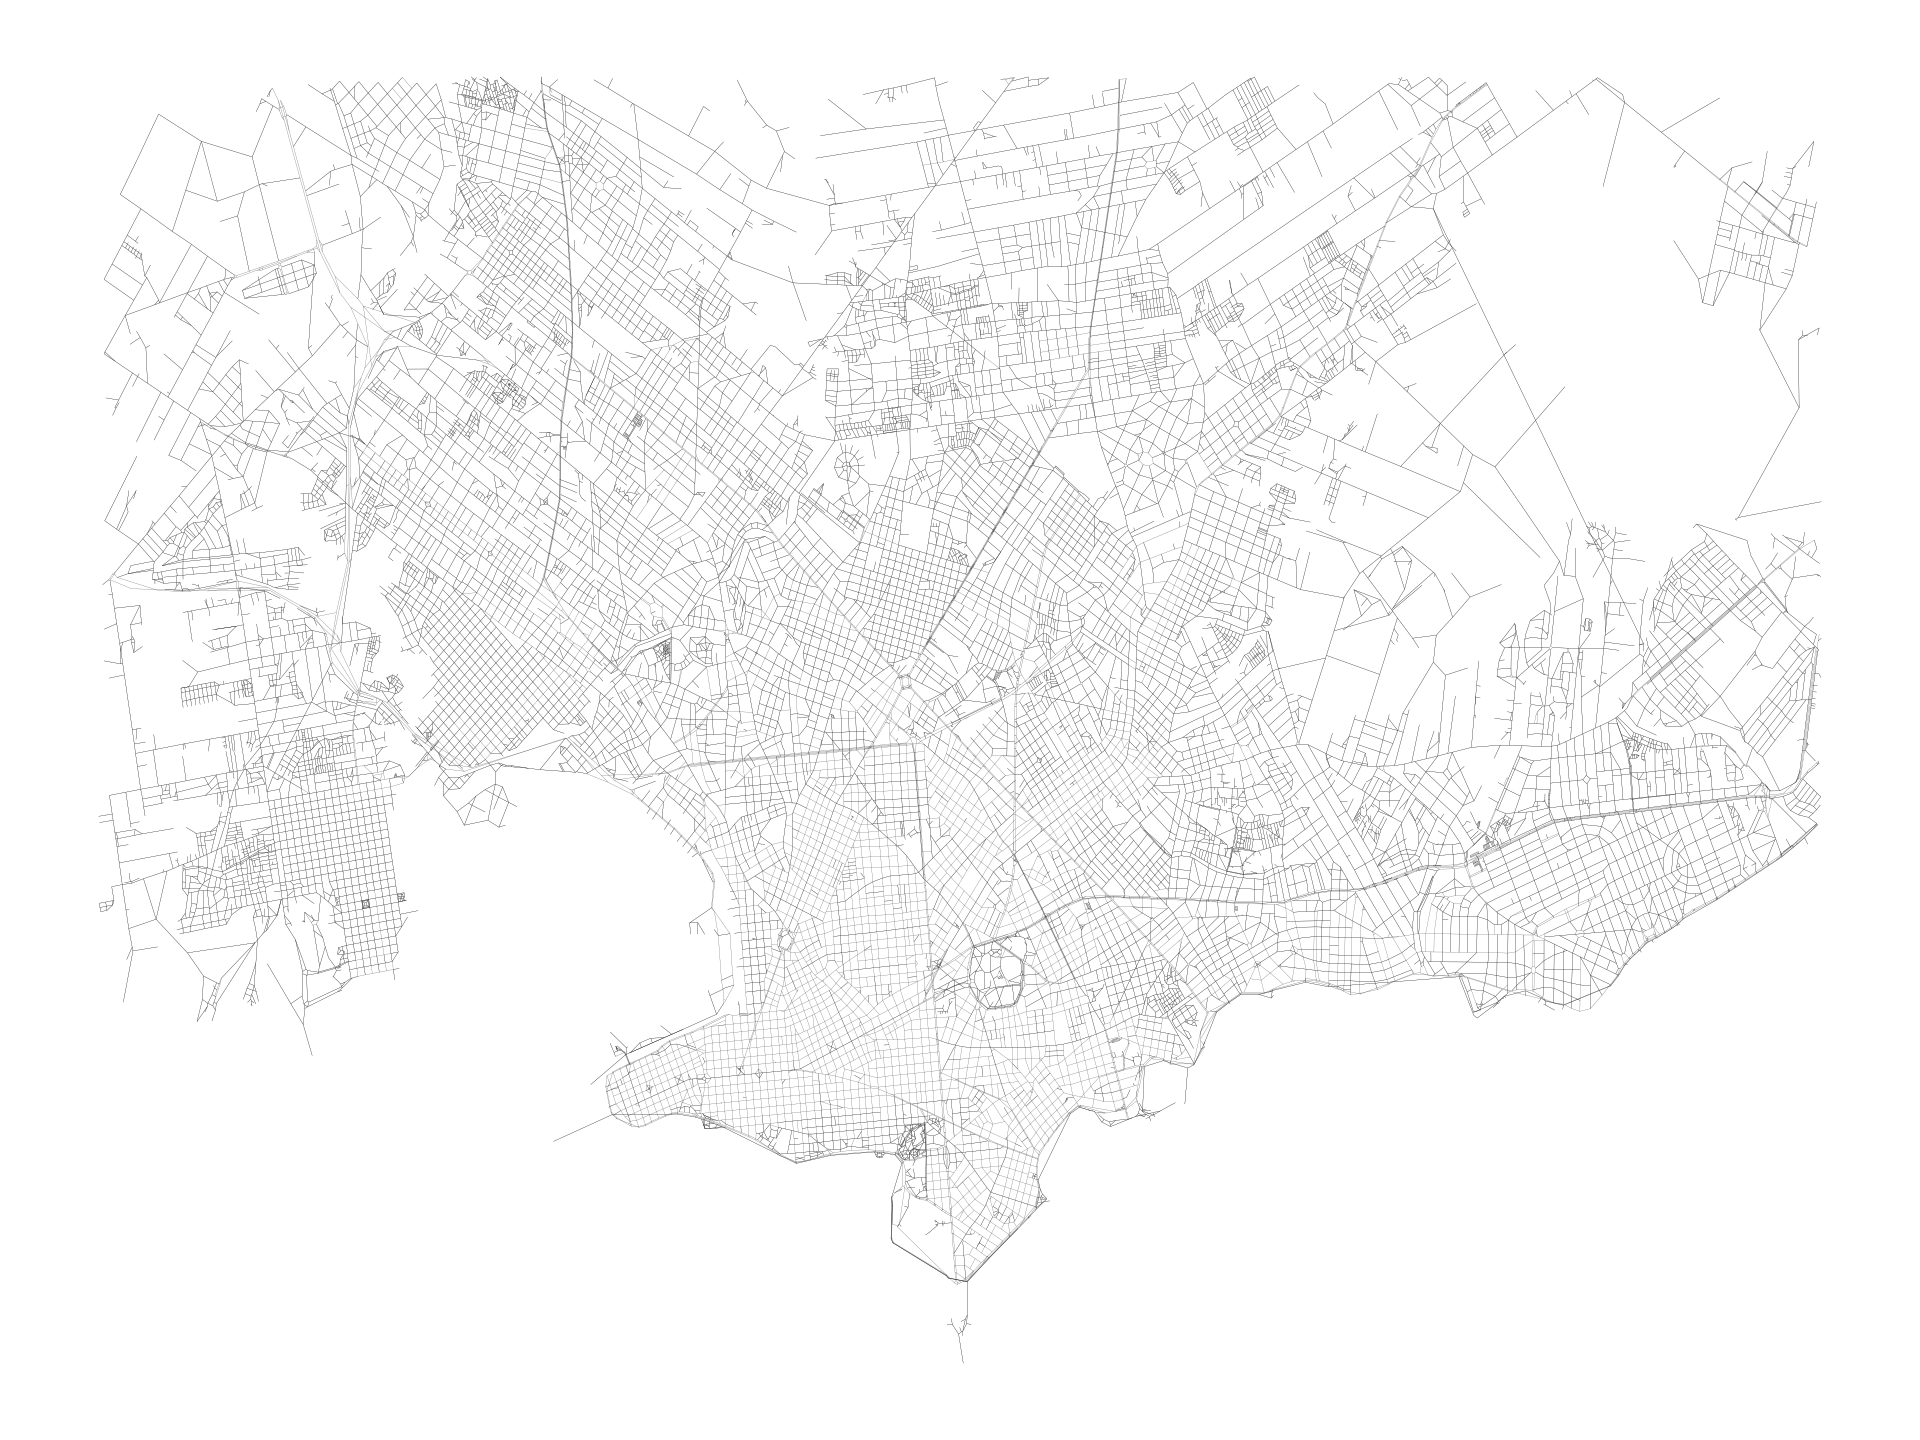
\includegraphics[width=10cm]{../resources/montevideo_full.png}
  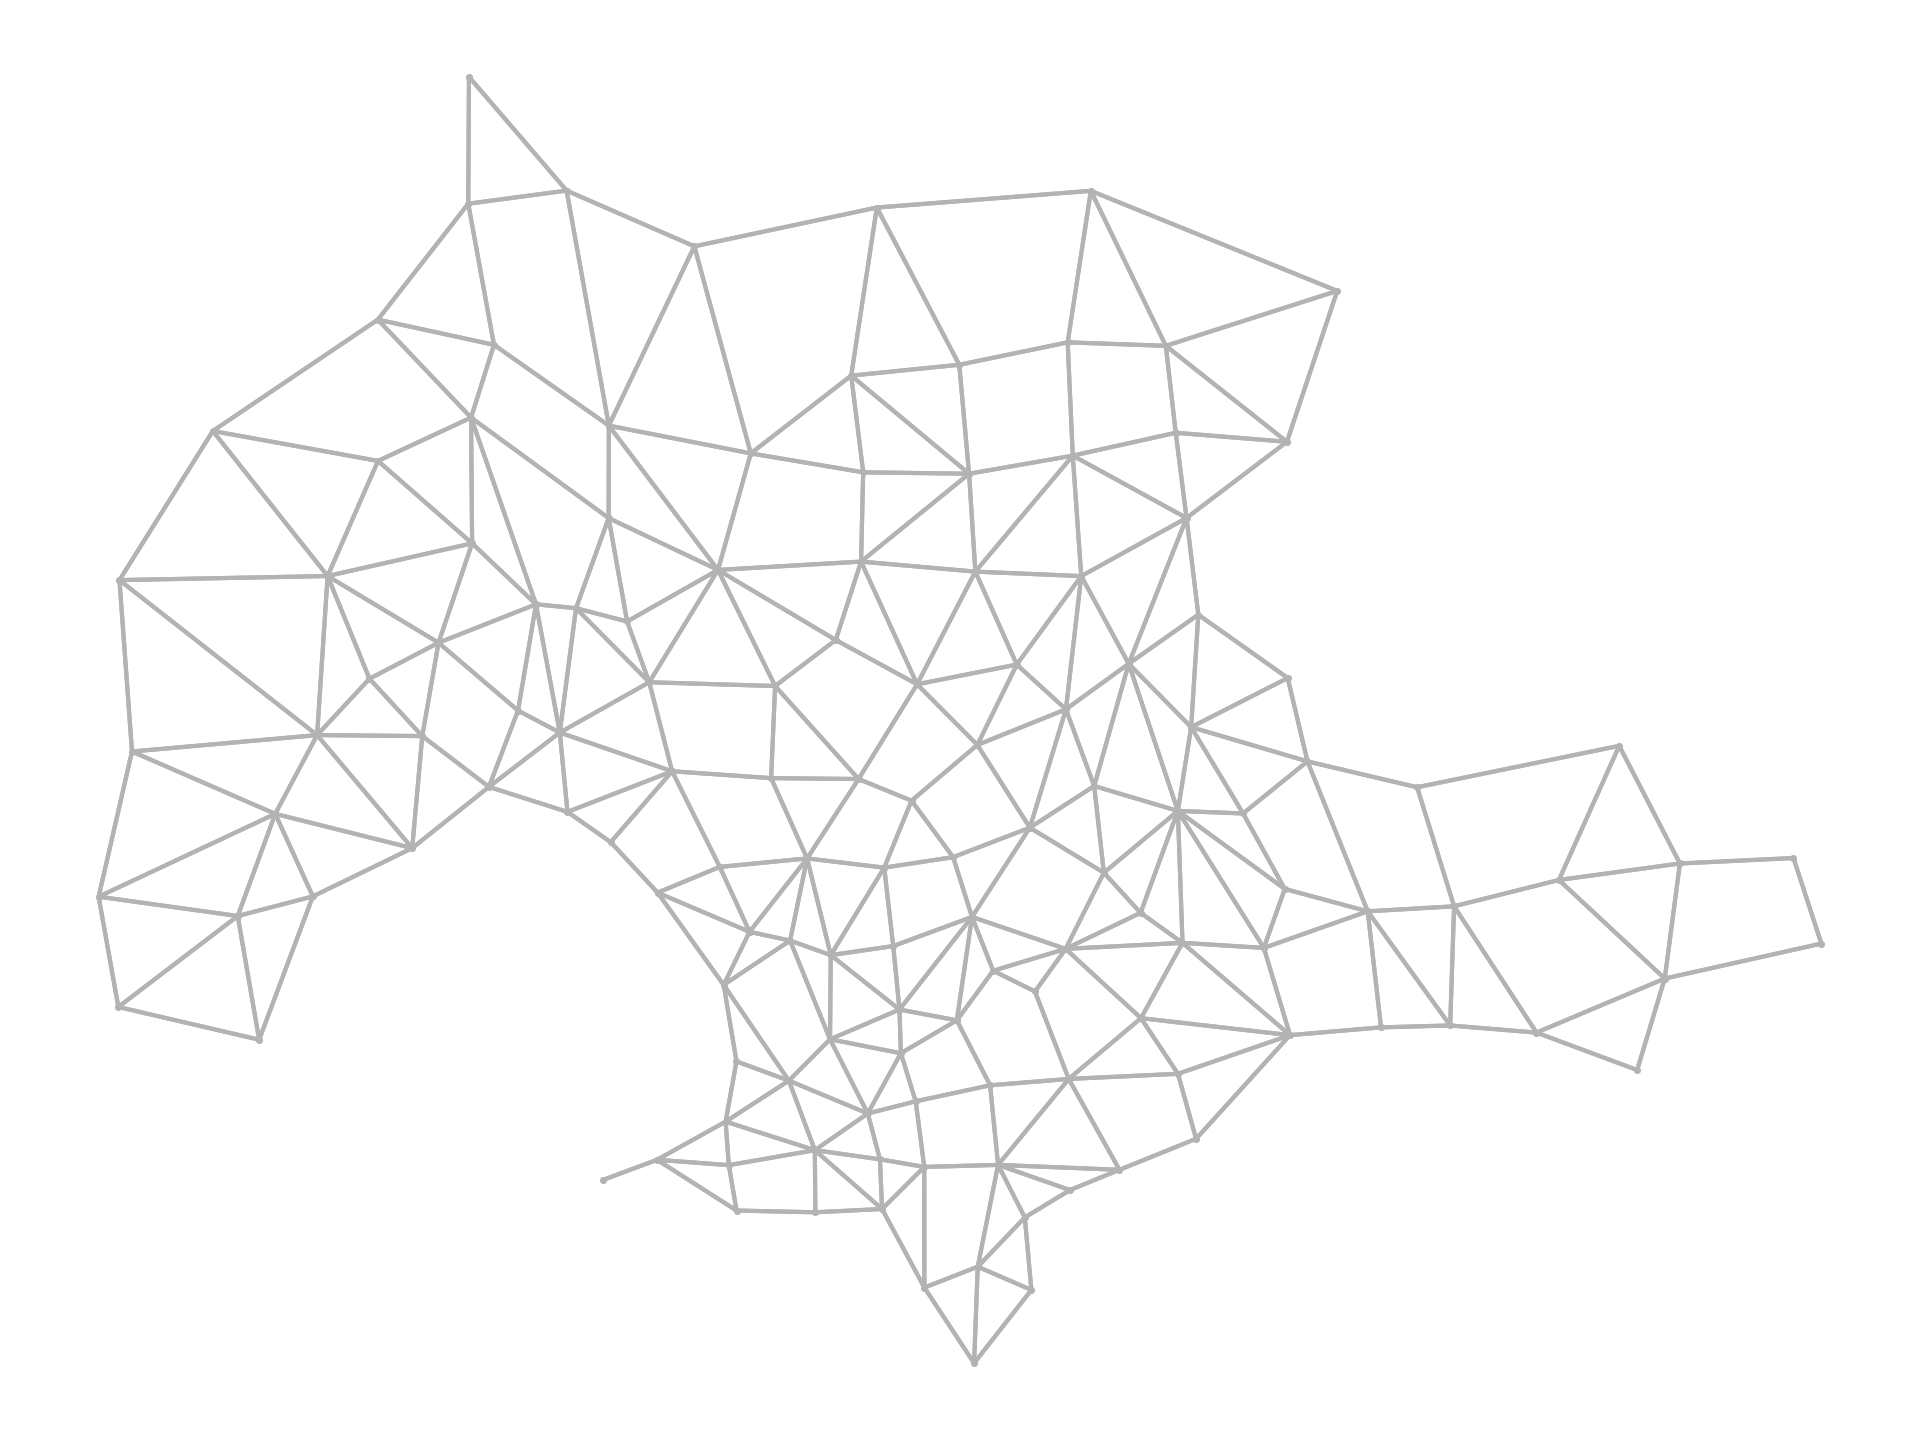
\includegraphics[width=10cm]{../resources/montevideo_simple.png}
  \caption{Compartiva de la red de calles de Montevideo y la red de la red utilizando la zonificación en 136 nodos y 636 arcos.}
  \label{fig:montevideosimplification}
\end{figure}

Actualmente la red de ciclovías en Montevideo abarca más de 48 km correspondiente a cerca de 1,27\% del largo total de la red de calles, ver Figura \ref{fig:montevideobikeways}. Se espera que esta red siga creciendo como parte de las políticas de incentivo del uso de la bicicleta que comprende 2,6\% del total viajes que se realizan \cite{Mauttone2017a}.

\begin{figure}[h!]
  \centering
  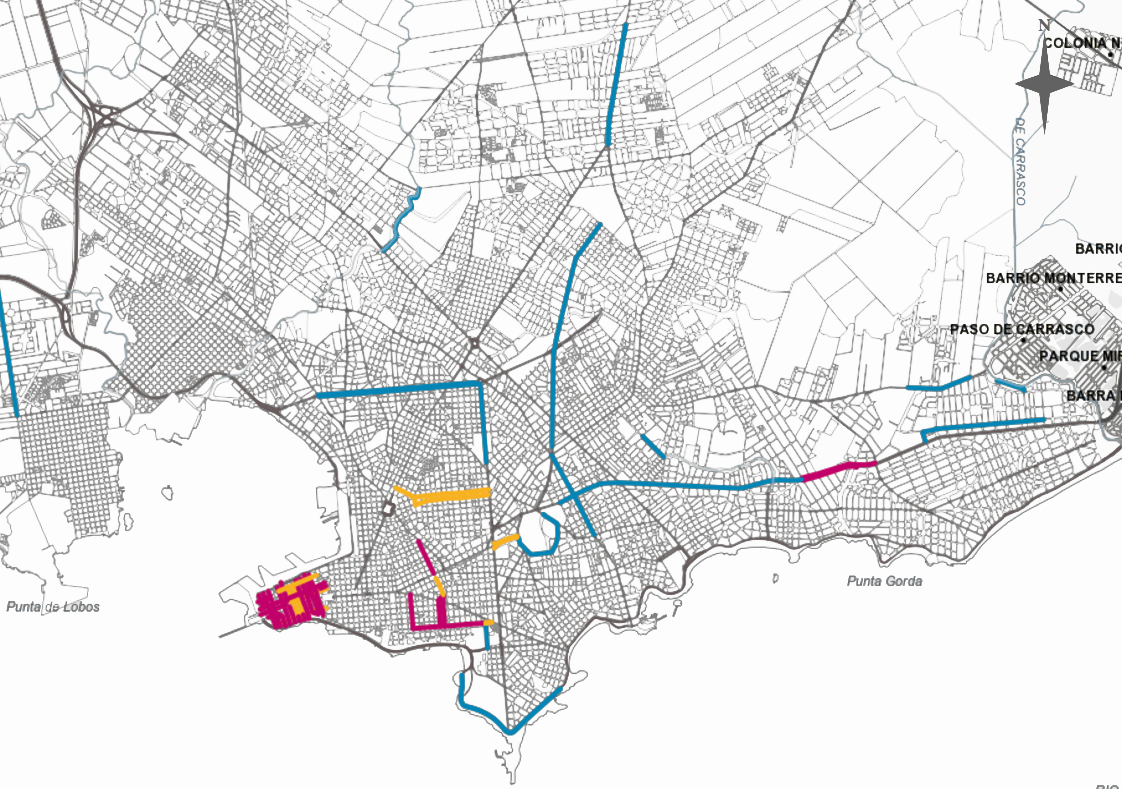
\includegraphics[width=10cm]{../resources/bicicircuitos_montevideo.png}
  \caption{Situación actual de la red de ciclovías en la ciudad de Montevideo. En color rojo se representa el tipo de tecnología más basico que en un límite de velocidad de 30 km/h para los vehiculos motorizados. En naranja la tecnología de nivel intermedio que a una senda específica para bicicletas dentro de la superficie de la calle. Por último, en azul, la tecnología superior correspondiente a una senda pavimentada exclusivamente construida para la bicicleta.}
  \label{fig:montevideobikeways}
\end{figure}

\subsection{Resultados}

Dado el tamaño de la instancia y los recursos computacionales disponibles decidimos utilizar 4 tipos de tecnología, incluyendo la base, y 10 puntos de quiebre. Probamos las funciones de transferencia de demanda logística y lineal y tres factores de presupuesto: 40\%, 80\% y 160\%. Las instancias fueron resueltas por el solver CPLEX versión 20.1.0.0, en un CPU Xeon Gold 6138 utilizando hasta 16 hilos y hasta 180 GB de memoria. CPLEX fue configurado para utilizar descomposición de Benders de manera automática, lo que nos permitió resolver de manera óptima las instancias estudiadas en unas pocas horas. Vale la pena mencionar que realizamos pruebas utilizando más tipos de tecnología y mayor cantidad de pares origen-destino pero nos encontramos con limitaciones en los recursos disponibles en términos de memoria o límite de tiempo de ejecución de 5 días.

El resumen de las ejecuciones se encuentra en la Tabla \ref{table:montevideoexecutions} y la asignación de presupuesto a cada tipo de tecnología de ciclovía en la Tabla \ref{table:montevideobudgetusage}. Observamos que los resultados son buenos en términos de demanda transferida para los casos con menor presupuesto en comparación con las instancias de Sioux-Falls. Podemos explicar esto porque la distribución de la proporción más significativa de la demanda en la red de Montevideo, como se puede ver en la Figura \ref{fig:montevideodemanddist}, se ubica en la misma región de la red. Por lo tanto concentrar la inversión en esa zona produce resultados de amplio impacto.

\begin{table}[h!]
  \centering
  \begin{adjustbox}{width=1.2\textwidth,center=\textwidth}
    \begin{tabular}{ccccccc}
      \toprule
        Instancia & \shortstack{Factor de \\ presupuesto} & \shortstack{Función de \\ transferencia} & \shortstack{\# Pares OD con \\ demanda transferida} & \shortstack{Demanda \\ transferida (\%)} & \shortstack{Tiempo de \\ ejecución \\ (hh:mm:ss)} \\
      \midrule
        1 & 0.4 & lineal & 395 & 53.92 & 02:59:57 \\
        2 & 0.4 & logística & 373 & 54.42 & 28:59:56 \\
        3 & 0.8 & lineal & 513 & 74.76 & 00:32:13 \\
        4 & 0.8 & logística & 510 & 75.76 & 00:37:32 \\
        5 & 1.6 & lineal & 598 & 94.7 & 00:14:26 \\
        6 & 1.6 & logística & 597 & 95.6 & 00:12:06 \\
      \bottomrule
    \end{tabular}
  \end{adjustbox}
  \caption{Resumen de ejecuciones sobre las instancias resueltas para la red de Montevideo.}\label{table:montevideoexecutions}
\end{table}

\begin{figure}[h!]
  \centering
  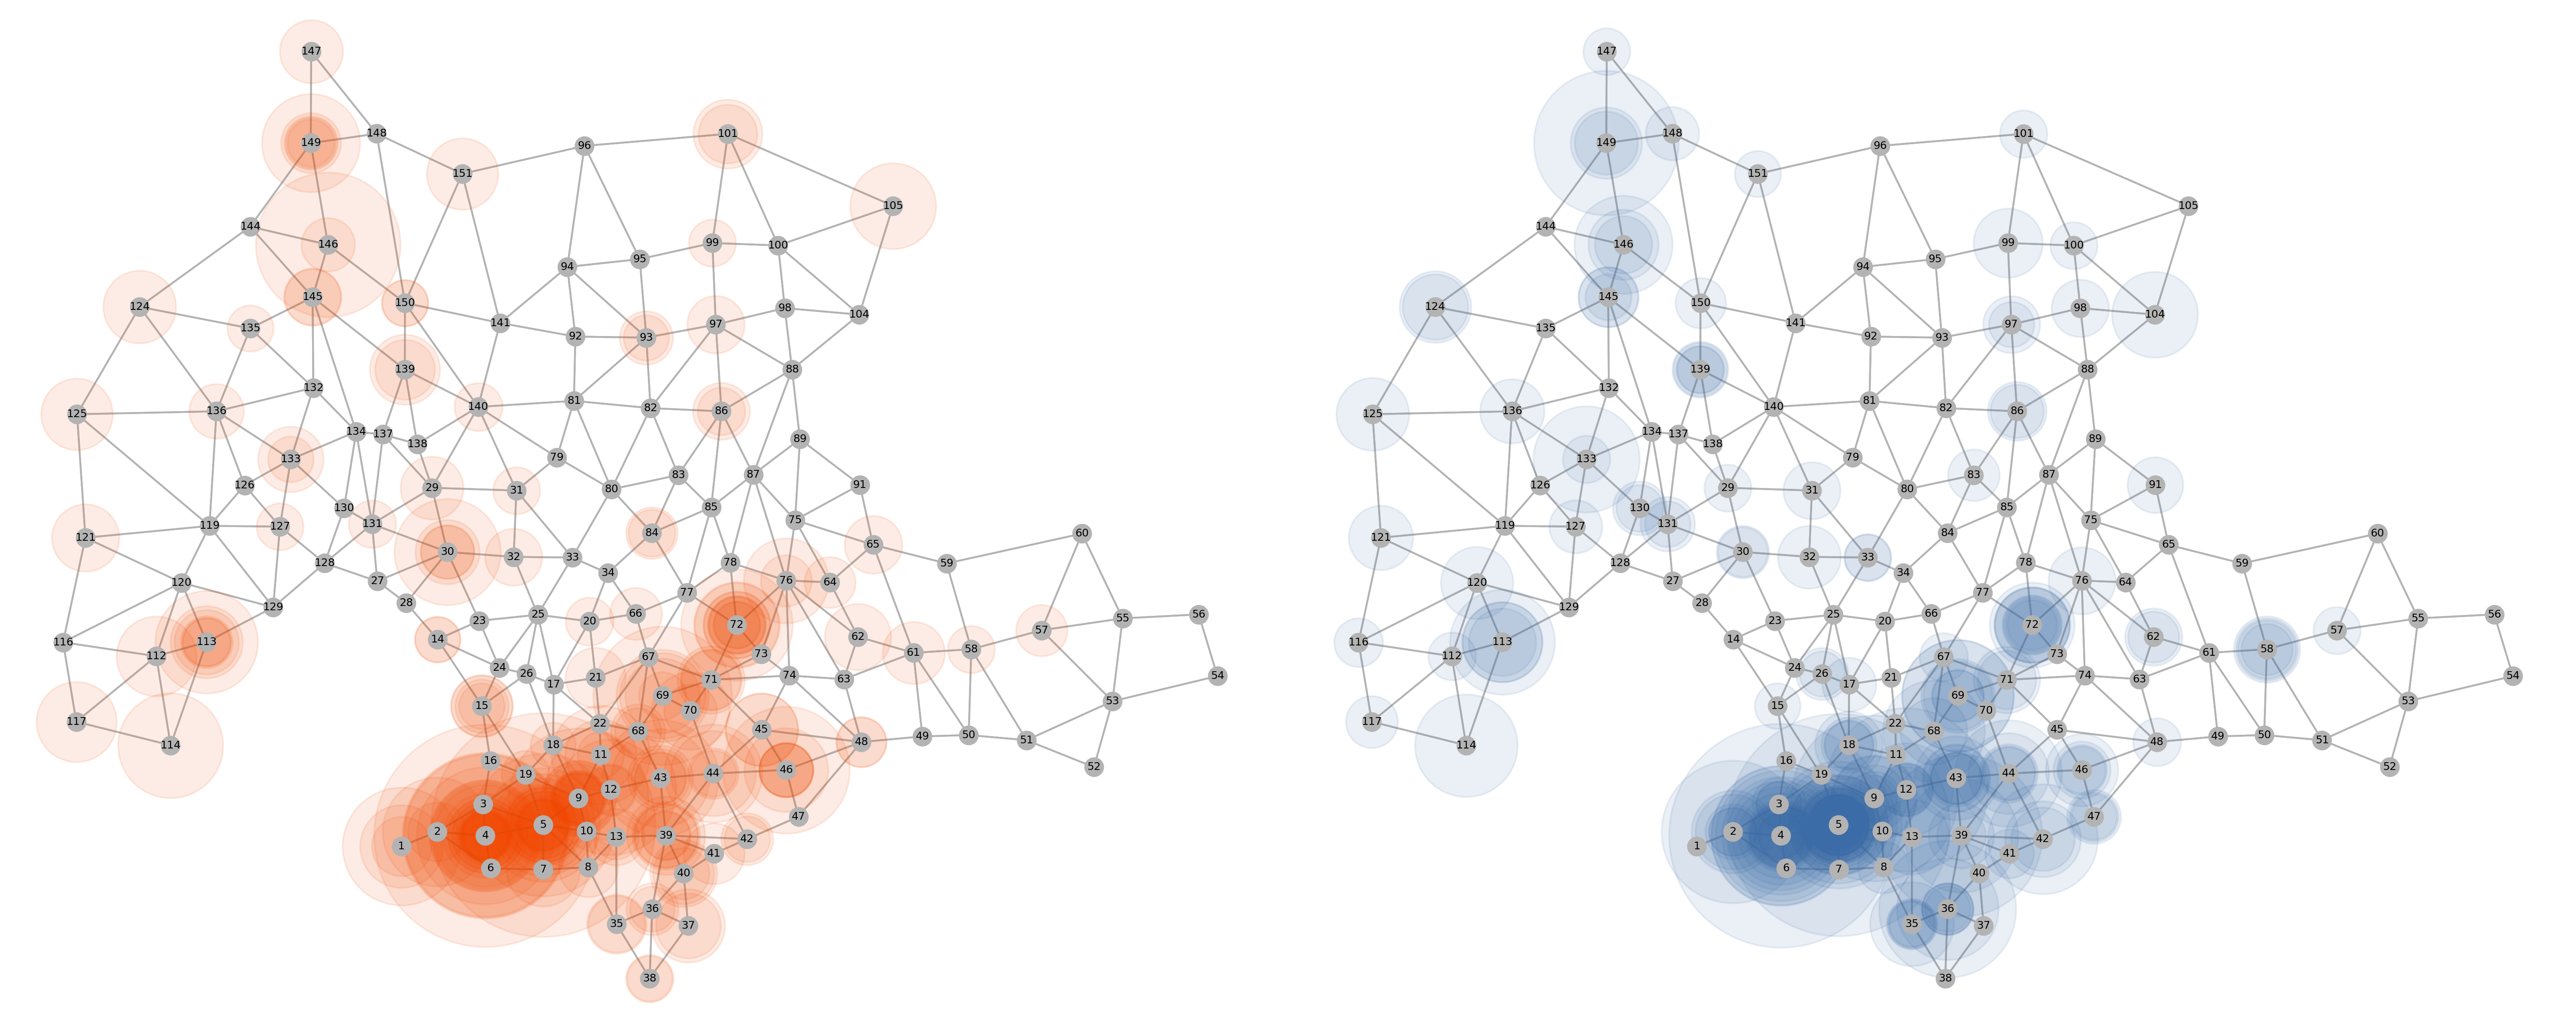
\includegraphics[width=12cm]{../resources/montevideo_demands.png}
    \caption{Representación de los 300 pares origen-destino con más demanda por ubicación de origen y destino. A la izquierda se ubican los orígenes y a la derecha los destinos. Los tamaños de los círculos son proporcionales al valor de demanda y no se suman por nodo. Estos pares origen-destino concentran casi el 60\% de la demanda total de los pares origen-destino considerados.}
  \label{fig:montevideodemanddist}
\end{figure}

Si comparamos las funciones de transferencia de demanda fijando el factor de presupuesto vemos que la lineal induce mayor transferencia y una red de ciclovías que afecta potencialmente a mayor cantidad de demanda por abarcar mayor proporción de la red de calles, ver Tabla \ref{table:montevideoinfracoverage}. Vemos que las ejecuciones con función de transferencia logística utilizaron mayor proporción del presupuesto en tecnologías más caras (Tabla \ref{table:montevideobudgetusage}), lo que lleva a una red de ciclovías más chica en términos de distancia. Por otro lado, si observamos la cantidad de pares origen-destino afectados por instancia vemo que la función logística fue más equitativa al afectar todos los pares origen-destino para todos los factores de presupuesto mientras que las instancias con función de transferencia lineal no lo hizo para ningún caso.

\begin{table}[h!]
  \centering
  \begin{adjustbox}{width=1.2\textwidth,center=\textwidth}
    \begin{tabular}{cccccc}
      \toprule
        Instancia & Presupuesto & \shortstack{Presupuesto \\ utilizado} & Tecn. 1 (\%) & Tecn. 2 (\%) & Tecn. 3 (\%) \\
      \midrule
        1 & 324220.24 & 323559.54 & 1.47 & 34.72 & 63.81 \\
        2 & 324220.24 & 321485.67 & 0.89 & 34.42 & 64.68 \\
        3 & 648440.47 & 647177.53 & 0.42 & 29.77 & 69.8 \\
        4 & 648440.47 & 647883.38 & 1.37 & 31.2 & 67.42 \\
        5 & 1296880.95 & 1296483.25 & 0.65 & 12.02 & 87.33 \\
        6 & 1296880.95 & 1296757.67 & 0.87 & 15.95 & 83.18 \\
      \bottomrule
    \end{tabular}
  \end{adjustbox}
  \caption{Proporción del presupuesto utilizado desagregado por tipo de tecnología para cada instancia. Debido al redondeo la suma puede no ser 100\% para algunas instancias.}\label{table:montevideobudgetusage}
\end{table}

\begin{table}[h!]
  \centering
  \begin{tabular}{ccccc}
    \toprule
      Instancia & Tecn. 1 (\%) & Tecn. 2 (\%) & Tecn. 3 (\%) & Total (\%) \\
    \midrule
      1 & 0.59 & 6.93 & 6.37 & 13.89 \\
      2 & 0.35 & 6.83 & 6.41 & 13.59 \\
      3 & 0.34 & 11.89 & 13.93 & 26.16 \\
      4 & 1.1 & 12.47 & 13.47 & 27.04 \\
      5 & 1.05 & 9.61 & 34.92 & 45.58 \\
      6 & 1.39 & 12.76 & 33.27 & 47.42 \\
    \bottomrule
  \end{tabular}
  \caption{Proporción del largo total de la red de calles en relación al largo total abarcado por cada tipo de tecnología.}
  \label{table:montevideoinfracoverage}
\end{table}

\begin{figure}[h!]
  \centering
  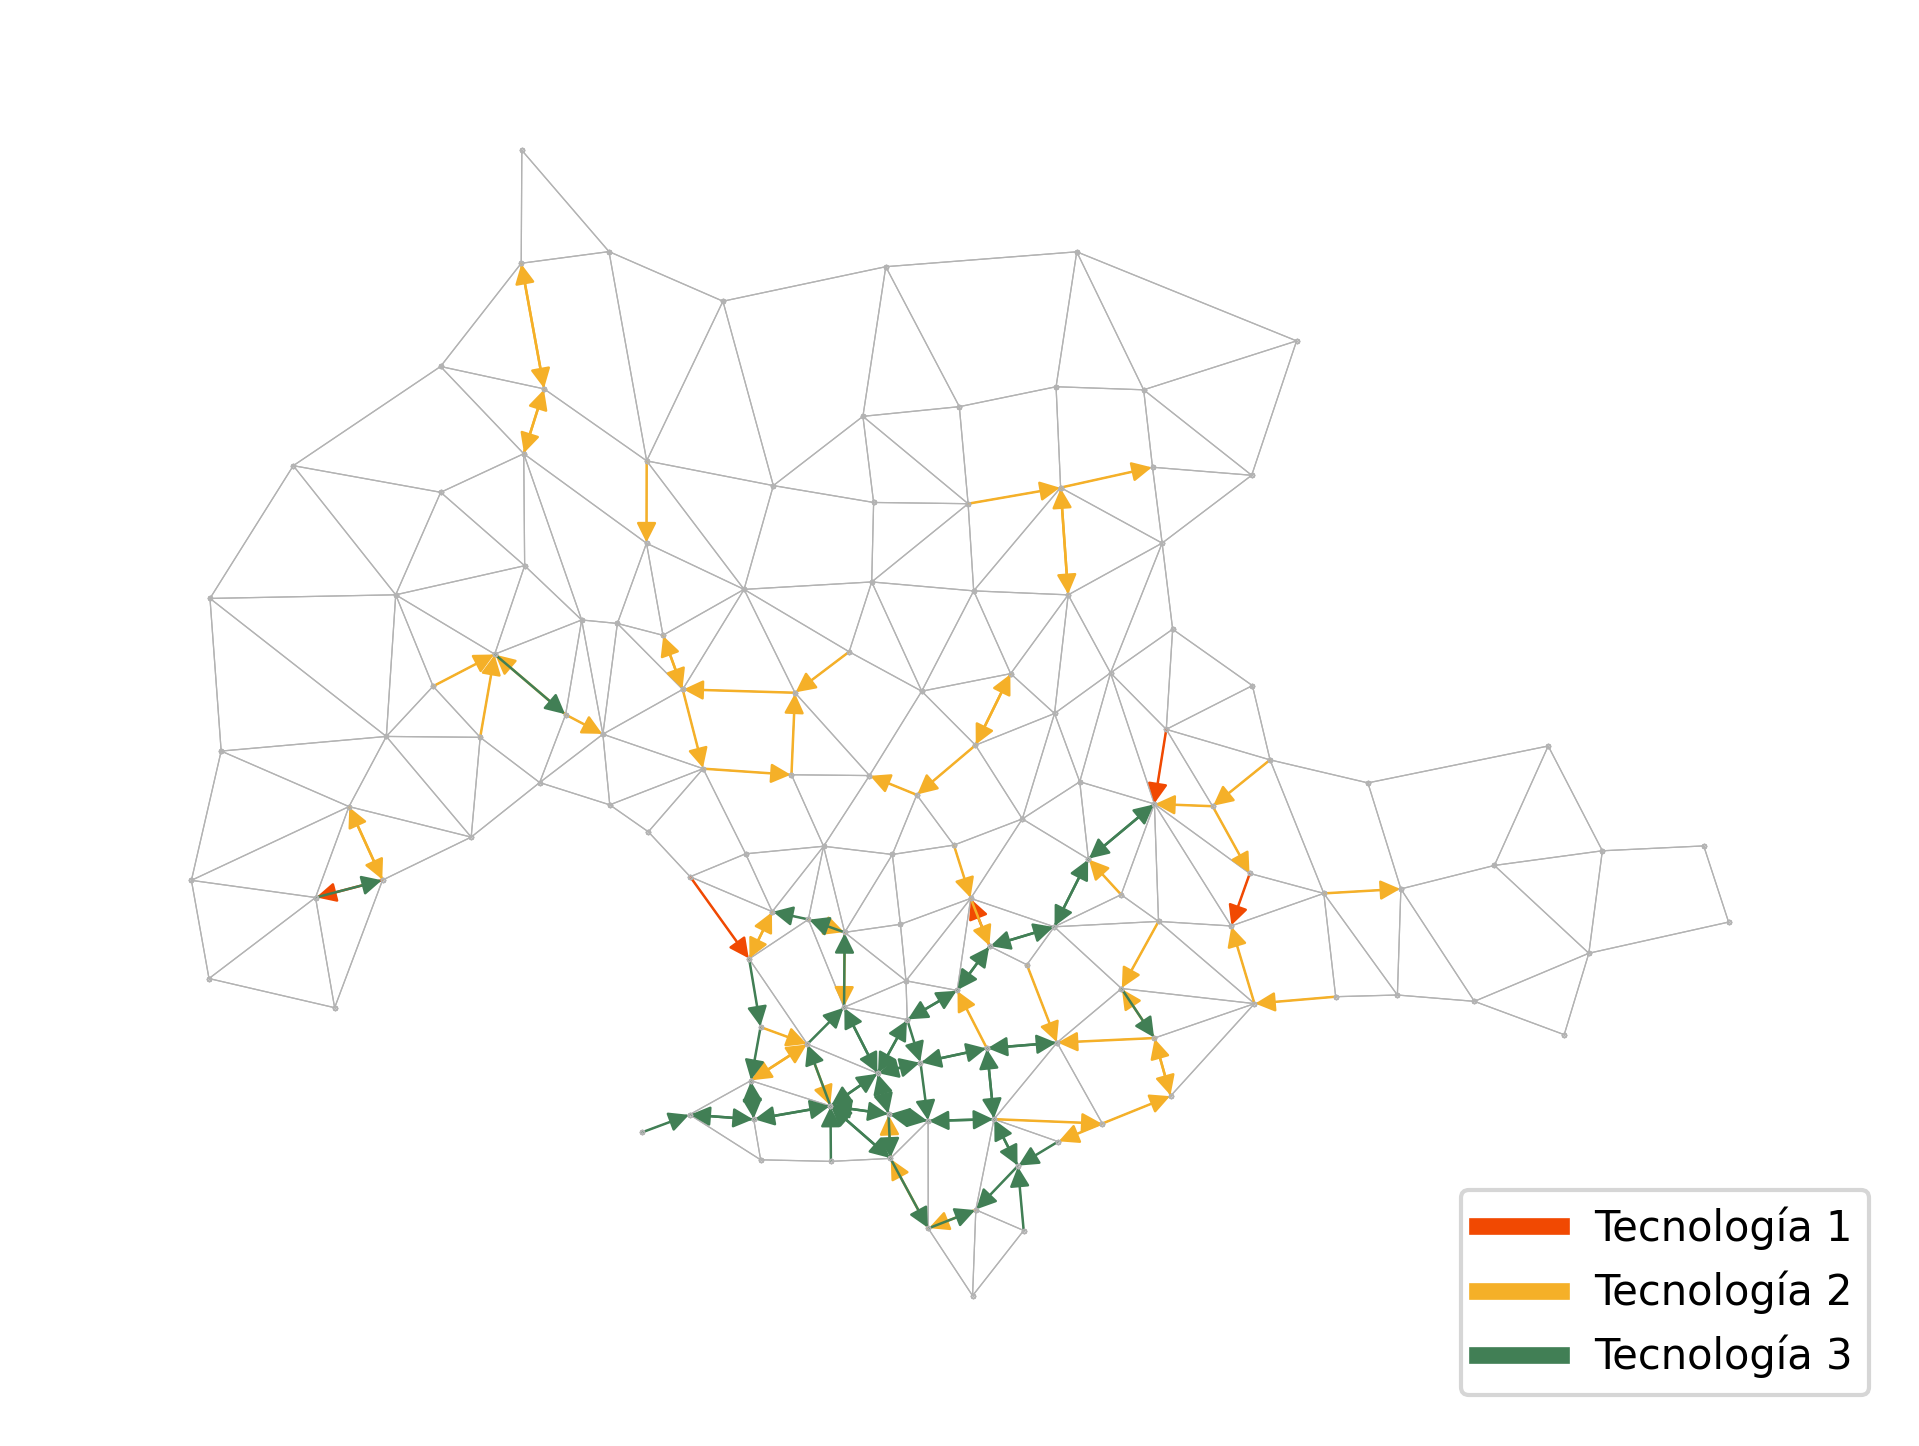
\includegraphics[width=6cm]{../resources/montevideo_d3000.0_linear_0.4_budget_factor.png}
  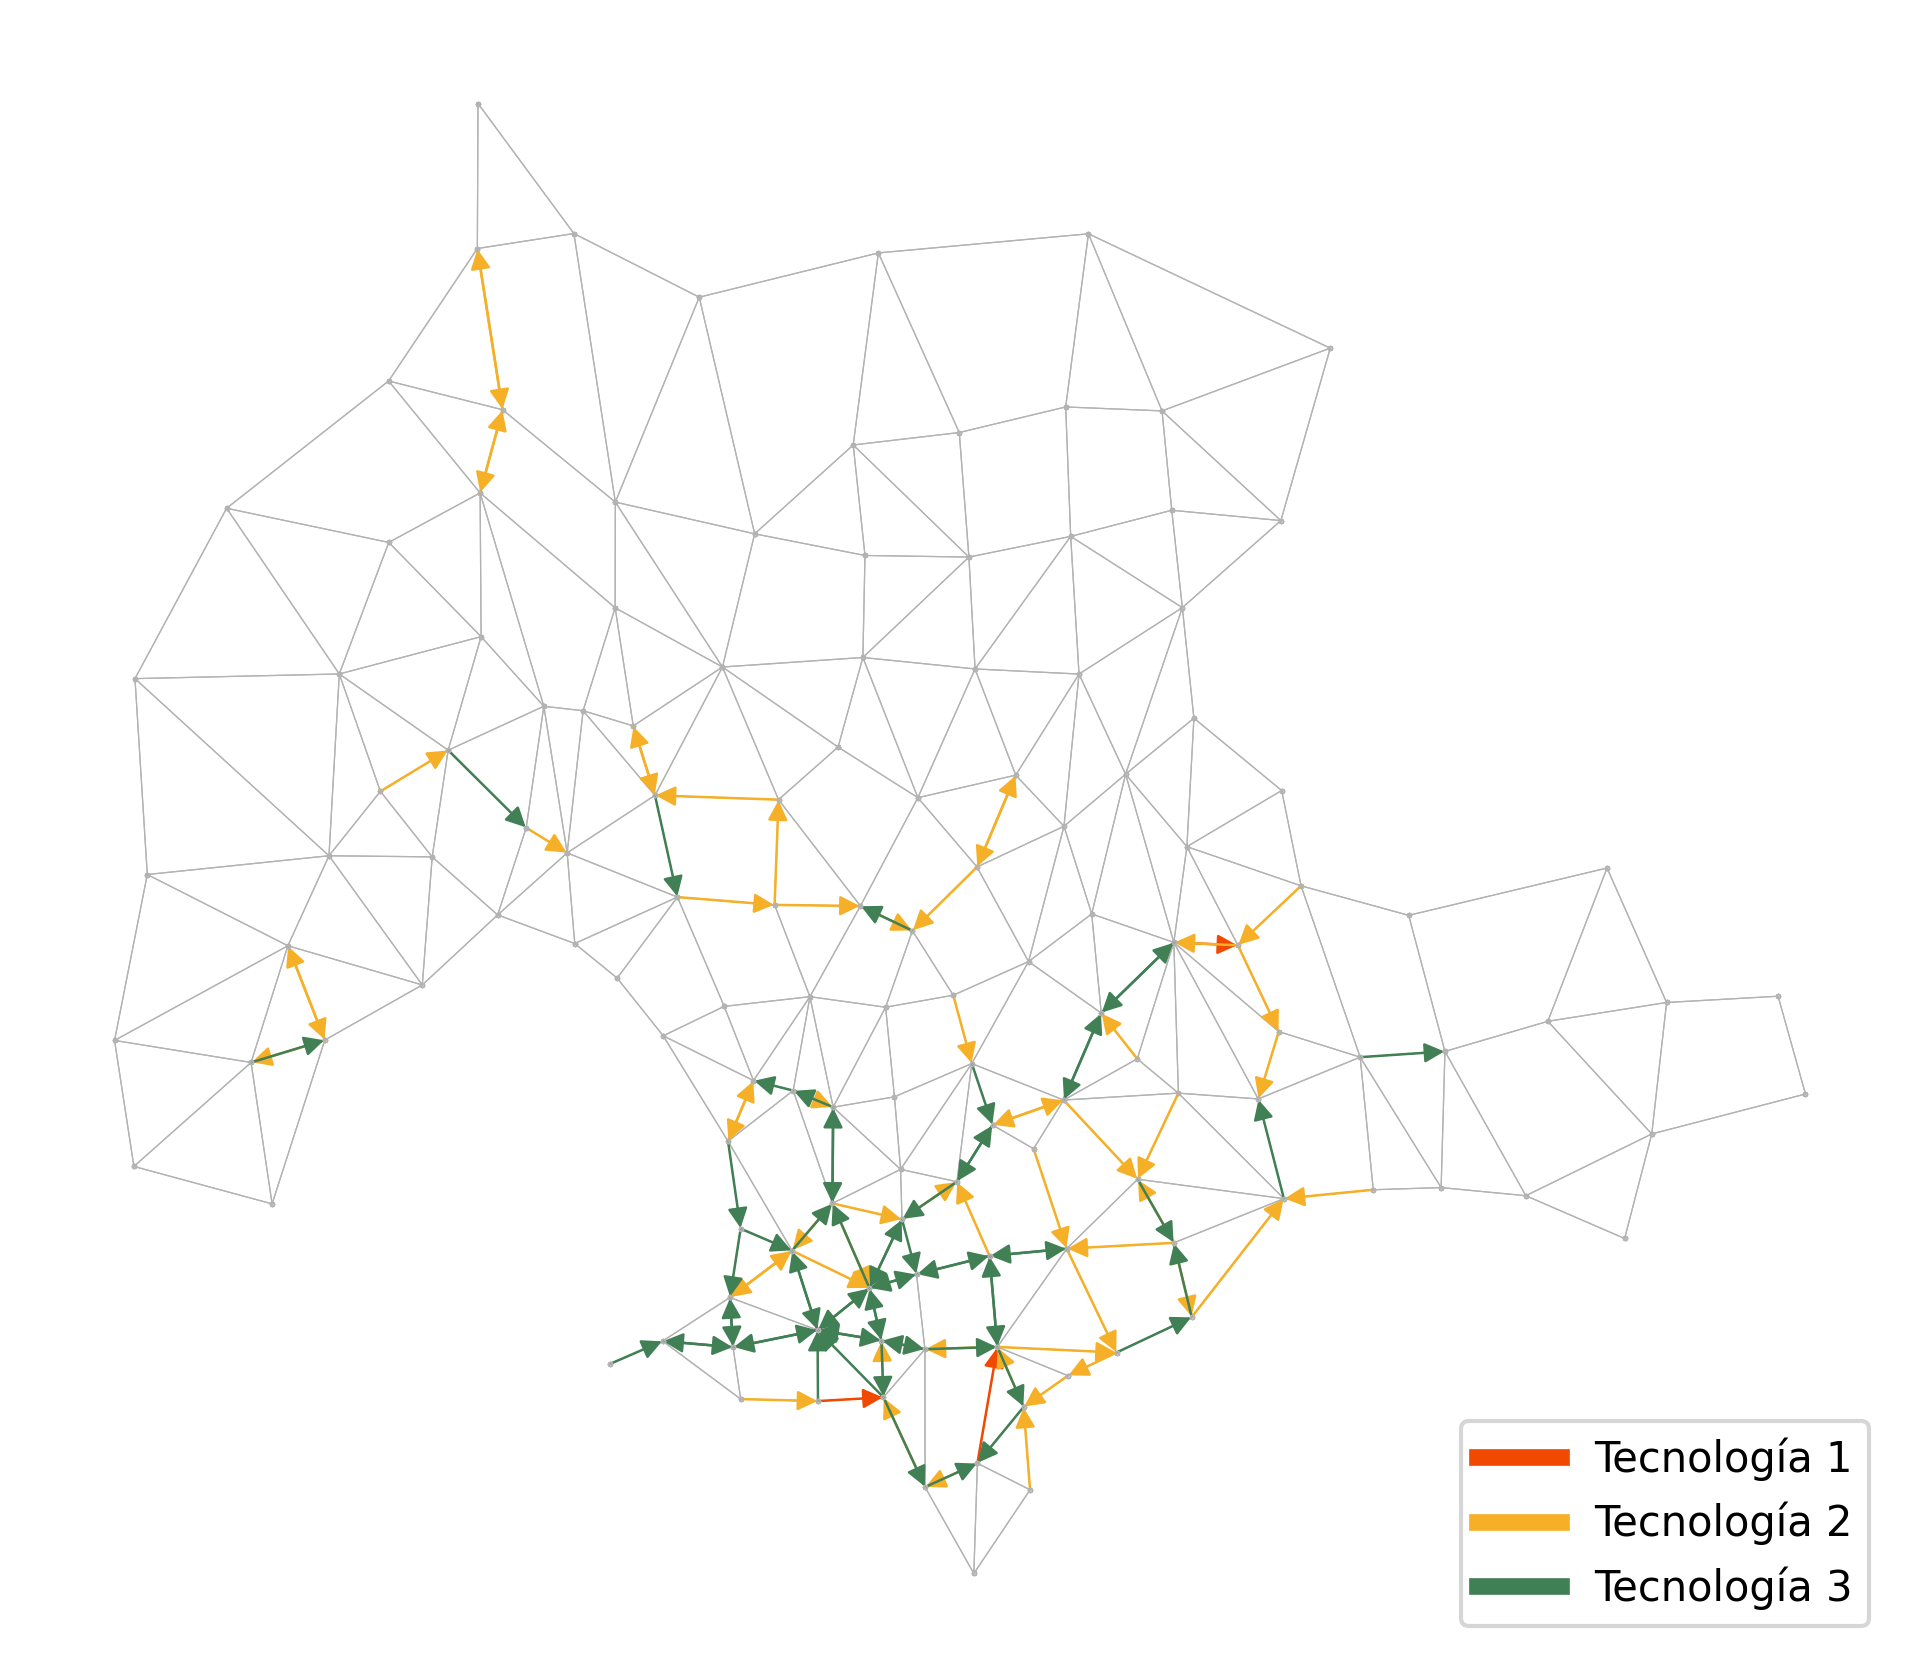
\includegraphics[width=6cm]{../resources/montevideo_d3000.0_inv_logit_0.4_budget_factor.png}
  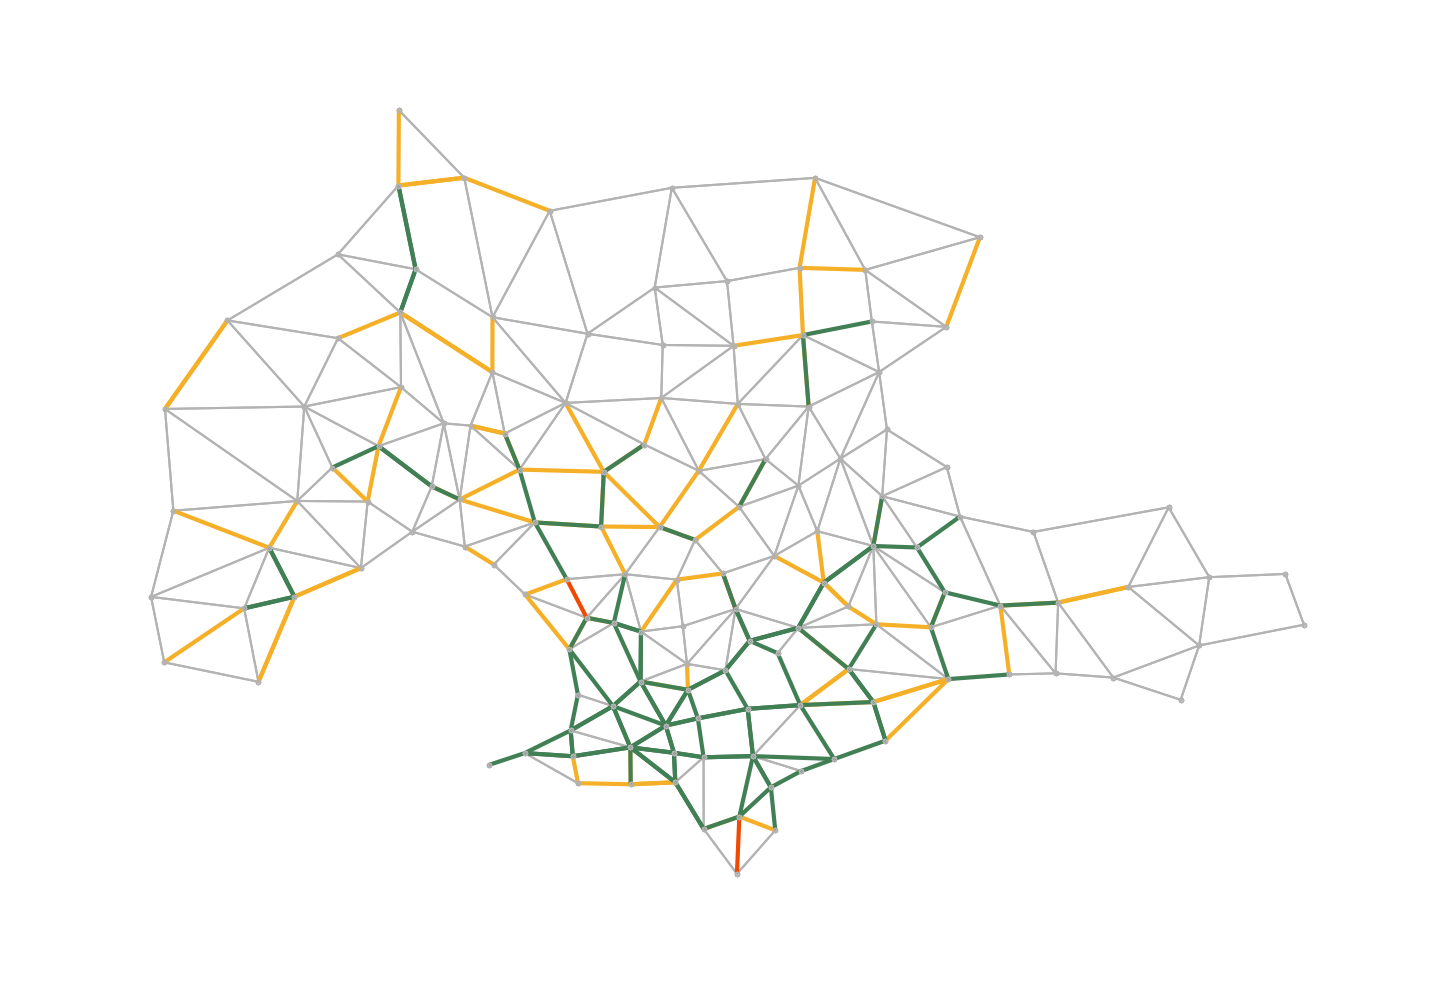
\includegraphics[width=6cm]{../resources/montevideo_d3000.0_linear_0.8_budget_factor.png}
  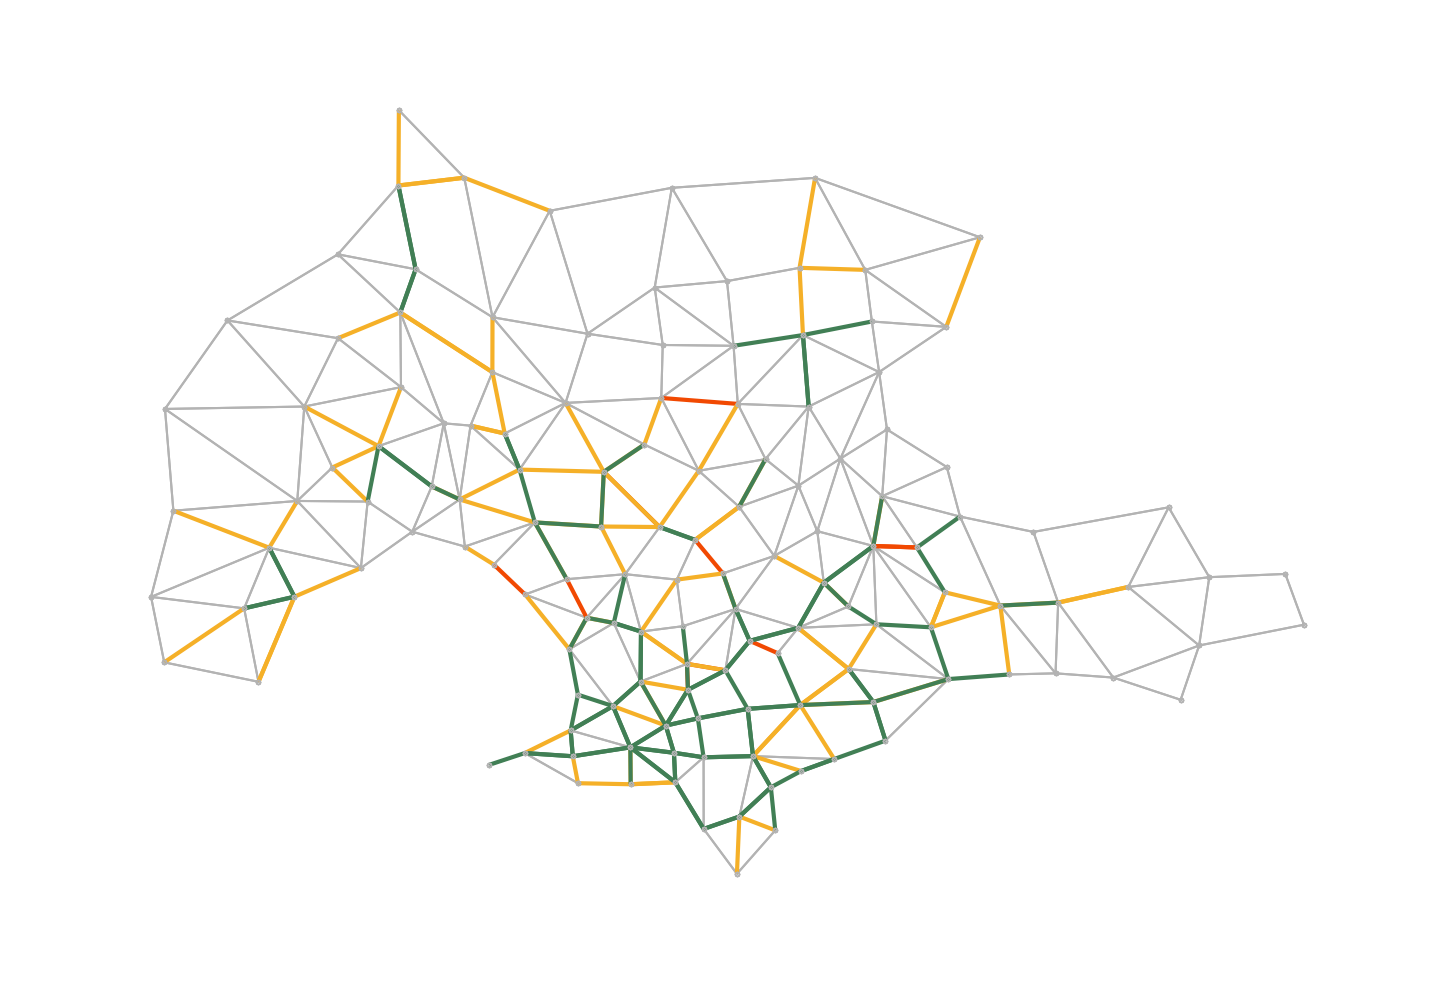
\includegraphics[width=6cm]{../resources/montevideo_d3000.0_inv_logit_0.8_budget_factor.png}
  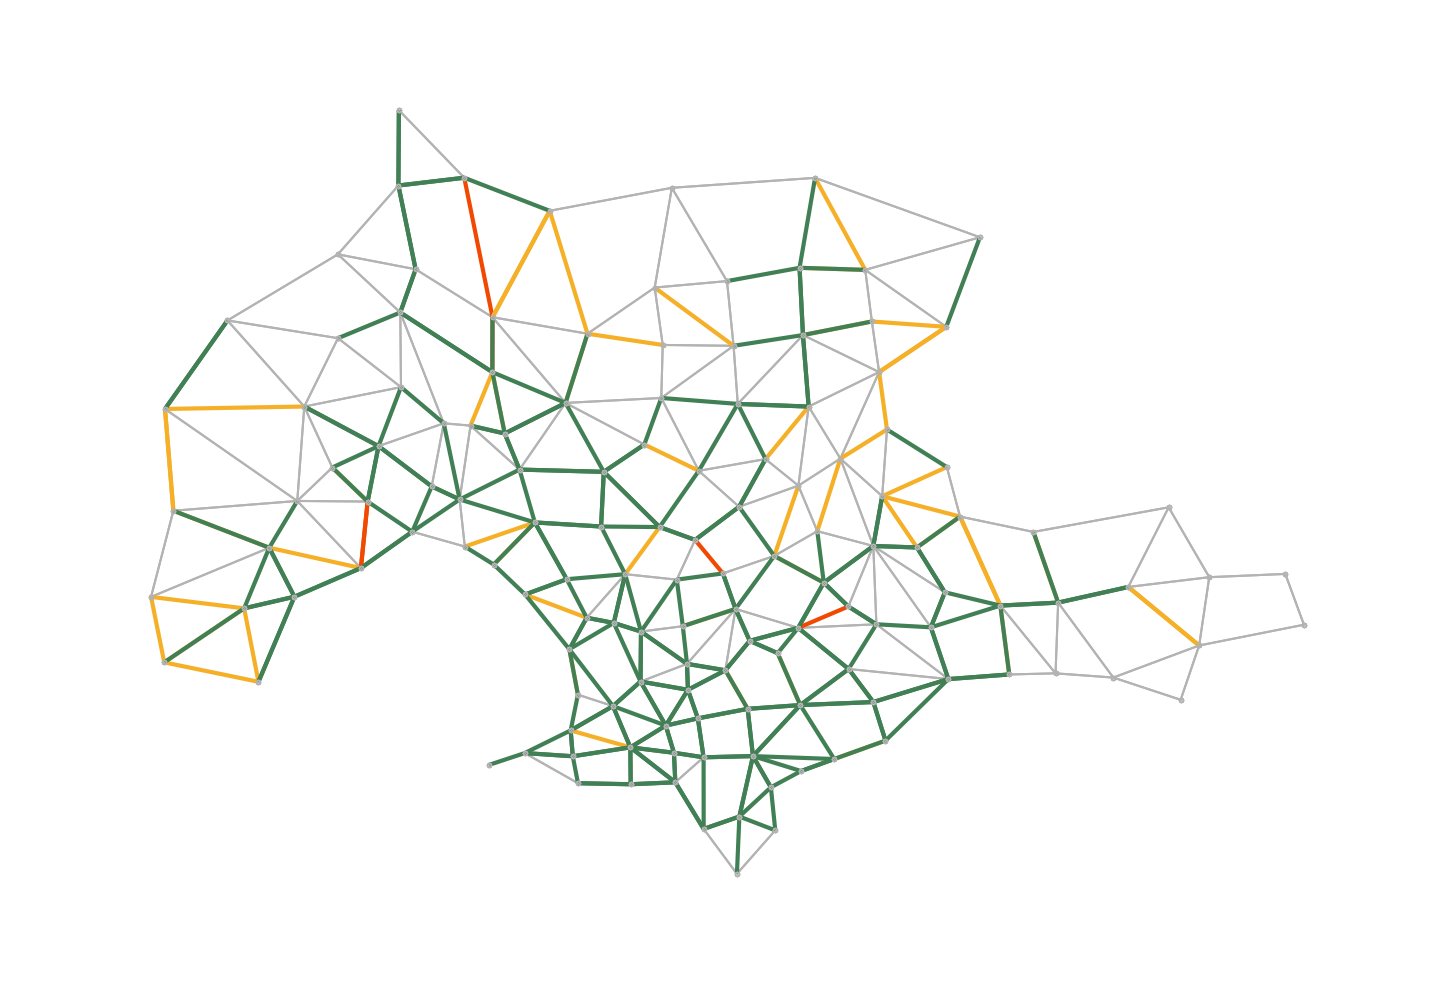
\includegraphics[width=6cm]{../resources/montevideo_d3000.0_linear_1.6_budget_factor.png}
  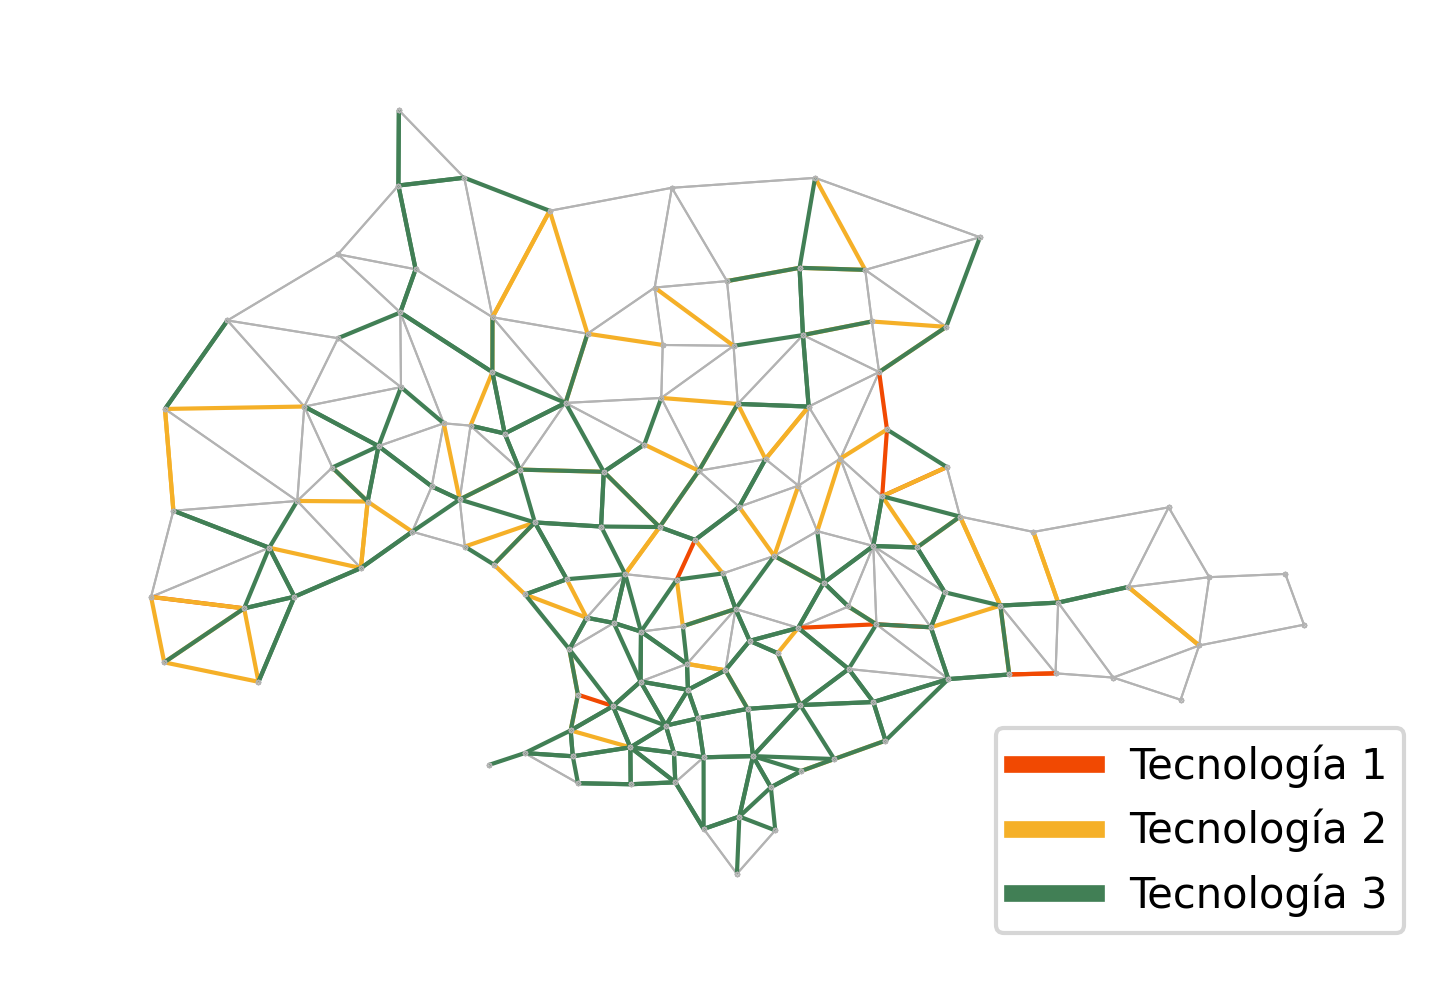
\includegraphics[width=6cm]{../resources/montevideo_d3000.0_inv_logit_1.6_budget_factor.png}
  \caption{Infraestructura de ciclovía construida para cada instancia. A la izquierda se ubican aquellas con función de transferencia de demanda lineal, a la derecha las que utilizan función logística. Además están dispuestas en orden creciente de factor de presupuesto desde arriba.}
  \label{fig:montevideo_instances_infras}
\end{figure}

Como análisis final, comparamos el desvío de los ciclistas respecto al camino más corto en distancia. Recordamos que en \cite{winters2010} el 75\% de los viajes en bici se desvían a lo sumo un 10\% del camino más corto y un 90\% se desvían hasta un 25\%. En nuestras instancias el desvío es menor y no podemos detectar ningún patron específico a menos de un aparente achatamiento de la curva de proporción de desvío hacia las instancias con mayor presupuesto asignado.

\begin{table}[h!]
  \centering
  \begin{tabular}{ccccccc}
    \toprule
      Instancia & 75\% & 90\% & 95\% & 98\% & Máximo \\
    \midrule
      1 & 1.0 & 1.0 & 1.1 & 1.17 & 1.46 \\
      2 & 1.0 & 1.08 & 1.11 & 1.17 & 1.43 \\
      3 & 1.0 & 1.0 & 1.08 & 1.18 & 1.43 \\
      4 & 1.0 & 1.04 & 1.1 & 1.17 & 1.41 \\
      5 & 1.0 & 1.0 & 1.0 & 1.1 & 1.42 \\
      6 & 1.0 & 1.0 & 1.01 & 1.1 & 1.33 \\
    \bottomrule
  \end{tabular}
  \caption{Proporción de desvío sobre el camino más corto en distancia para cada instancia con percentiles por cantidad de demanda. El cálculo se hizo considerando los pares origen-destino para los cuales hay demanda transferida, ordenandolos por factor de desvío y calculando los percentiles por cantidad de viajes sobre la demanda transferida total. Por lo tanto es la misma medida que \cite{winters2010}.}
  \label{table:montevideoshortestpathdeviation}
\end{table}

  \chapter{Conclusiones y trabajo a futuro}

Proponemos una nueva variante del problema de diseño de redes de ciclovías consideramos varios tipos de tecnologías de ciclovías, que implican diferentes costos de construcción y costos de usuario. Tiene la particularidad que la no construcción es ciclovías es una solución factible que consideramos razonable y realista. Permitimos modelar el comportamiento de la demanda de manera que pueda adaptarse a diferentes realidades mediante la especificación de funciones de transferencia de demanda particulares. La demanda considerada puede transferirse a la bicicleta desde otros modos y esta transferencia ocurre si la ciclovía construida permite a los usuarios circular por caminos de menor costo en relación a la situación inicial. Estas últimas características son la principal diferencia con trabajos anteriores y pueden ser considerados los principales aportes a la comunidad académica. Lo abordamos como un problema de optimización utilizando como marco conceptos consolidados en área de Investigación Operativa como el diseño de redes {\it Multi-Facility, Multi-Commodity} y {\it piecewise linear costs}. Todas estas características en conjunto lo diferencian de otros trabajos en los que ya se han abordado algunos de estos puntos.

Durante el desarrollo del trabajo consideramos varias alternativas para su formulación: binivel, MILP de un único objetivo y MILP multiobjetivo. Nos decidimos por el último ya que buscábamos un método de resolución exacto que sea aplicable a instancias de características realistas. Pese a la complejidad de nuestro modelo, este logra resolver correctamente instancias de tamaño medio en tiempo razonable aunque la instancia de la red de Montevideo junto a los parámetros utilizados estaban en el límite del tamaño manejable por el solver utilizado dado que cualquier incremento en cantidad de tipos de tecnologías o cantidad de pares origen-destino disparaban los tiempos de ejecución o utilización de recursos más allá de lo permitible para este trabajo. Sin embargo, dado que el problema es de planificación estratégica a largo plazo, en una aplicación real el tiempo de ejecución no es tan determinante y se podrían asignar recursos excepcionales llegada la necesidad sin olvidar que estamos trabajando sobre un problema de complejidad NP.

Si bien el modelo fue pensado para el diseño de ciclovías desde cero, puede contemplar el problema de mejora de una red de ciclovías asignando un costo de construcción cero a la tecnología que se encuentre construida. Esto es posible dado que modelamos los costos por arco y tecnología pese a que luego especificamos los parámetros de manera general solamente en función del tipo de tecnología y el largo del arco.

Mediante la realización de experimentos numéricos en una instancia chica y una instancia de la ciudad de Montevideo, basados en datos fundados, mostramos que es posible construir una red de ciclovías que induce una buena medida de demanda transferida a la bicicleta incluso con lo que se considera bajos factores de presupuesto. De nuestras pruebas concluimos que utilizar mayor cantidad de puntos de quiebre favorece tanto la demanda transferida total como decisiones más inteligentes en términos de infraestructuras construidas a razón de un mayor costo computacional. También concluimos que la función de transferencia de demanda que se utilice es relevante en los resultados en varios aspectos además de la demanda transferida, por ejemplo cantidad de pares origen destino afectados y factor de desvío de los caminos de menor costo de usuario sobre los caminos de menor distancia.

Como variantes posibles, pensamos que si bien permitimos modelar funciones de transferencia de demanda arbitrarias vale la pena mencionar que se puede desarrollar una versión más eficiente para la función de transferencia lineal mediante la representación explícita de la función de transferencia en la función objetivo sin utilizar el mecanismo de los puntos de quiebre. Además, esta versión no necesitaría ser multiobjetivo dado que la representación de la función de transferencia sería estrictamente decreciente. Otro enfoque para modelar la demanda que se transfiere a la bicicleta es mediante los modelos de elección discreta siguiendo el trabajo \textcite{Pacheco2021}, cambiando la función objetivo para que maximice la cantidad esperada de utilización de la bicicleta. Además, se pueden contemplar otros aspectos en los costos o utilidad percibida por los usuarios respecto a los trayectos en bicicleta, por ejemplo la distancia total y distancia fuera de la red de ciclovías. Otros conceptos con los que podemos extender nuestro modelo son: contemplar las discontinuidades en los tipos de tecnologías \parencite{baya2021} durante un trayecto en bicicleta, integrar el concepto de camino seguro de manera que la demanda entre un origen y un destino pueda potencialmente ser satisfecha solo si existe una ciclovía que los une \parencite{Duthie2014}, y permitir distinguir qué tipos de tecnologías se puede construir en cada arco de la red, aspecto que puede ser necesario para contemplar las diferentes realidades dentro de una ciudad. También se podría adaptar el modelo a un enfoque de bicicletas compartidas, realidad que es común en otras partes del mundo y requiere tener en cuenta los centros de estacionamientos requeridos para este sistema \parencite{vogel2016}.

Entendemos que seguir agregando complejidad al modelo puede resultar en que sea inaplicable debido a los altos tiempos de ejecución dado que en la situación actual ya nos encontramos con un límite en el generoso hardware con el que dispusimos. Identificamos dos alternativas para circunvalar esta situación: solucionar el problema de manera aproximada con una metaheurística o reestructurar la formulación de manera de aplicar el algoritmo de descomposición de Benders \parencite{bucarey2022, crainic2021} lo que puede mejorar los tiempos de ejecución de la resolución exacta.

Respecto a los datos, en este trabajo estimamos y aproximamos muchos de los parámetros. Puede ser interesante utilizar datos más precisos para este problema, por ejemplo, una matriz de demanda que considere varios modos de transporte. Por otro lado podemos comparar las soluciones del modelo en términos de demanda transferida contra un escenario real de dos formas: la más costosa es mediante encuestas, suponiendo que cierta infraestructura es construida, enfoque similar a \textcite{shwe2014}; la otra es contrastar los resultados del modelo contra datos de ciudades que mantengan un histórico sobre la utilización de la bicicleta y cobertura de ciclovías.


  \backmatter % Comando que generalos apéndices, anexos y bibliografía. NO COMENTAR

  \printbibliography[heading=bibintoc,title={Referencias bibliográficas}]
  \bibend % No comentar

  \glosario % Glosario, NO comentar

  \apenarabicnumbering
  \apenmatter % Apéndices, NO comentar
  \chapter{Validación de la formulación binivel}
\label{sect:apendixbilevelvalidation}

Para discutir la validez matemática del modelado binivel (\ref{eq:objective1lvl})-(\ref{eq:flowbalance}), definida en el Capítulo \ref{sect:problemdefinition}, partimos de una formulación estándar de BLPP lineal, como se puede encontrar en Bard \cite{bardbook} y demostramos la validez en base a las definiciones ahi mencionadas justificando según nuestra formulación. Sea la siguiente formulación simplificada del problema binivel:

\begin{align}
\max_{y \in Y}            & \; F(x, y) \label{bilevelgeneric1} \\
\modelspace \text{s.t.}\; & A_1 x + B_1 y \leq b_1 \\
                          & y \geq 0 \\
                          & \min_{x \in X} f(x, y) \\
                          & \modelspace A_2 x + B_2 y \leq b_2 \label{bilevelgeneric5} \\
                          & \modelspace x \geq 0 \label{bilevelgeneric6}
\end{align}

Y las siguientes definiciones:

\begin{definition}
Conjunto factible
\begin{align}
  S = \{(x, y) \setminus x \in X, y \in Y, A_1 x + B_1 y \leq b_1, A_2 x + B_2 y \leq b_2 \}
\end{align}
\end{definition}

\begin{definition}
Conjunto de reacción del segundo nivel:
\begin{align}
  P(y) = \{ x \in \text{argmin}_{\hat{x} \in X} f(\hat{x}, y) : A_2 \hat{x} + B_2 y \leq b_2 \}
\end{align}
\end{definition}

Diremos que el problema está bien formulado si el conjunto $S$ es no vacío, es decir, si existen soluciones factibles y se cumple que para toda $y$ el conjunto $P(y)$ es no vacío, en otras palabras, si para todo movimiento del problema de primer nivel, hay margen de decisión en el segundo nivel.

\begin{lemma}$S$ es no vacío
\end{lemma}

\begin{proof}
$S \neq \emptyset$ ya que $\exists (x_0, y_0) \in X \times Y$ donde $y_0$ es el vector $y_{ai_0} = 1 \forall a \in A$, $i_0$ es la tecnología cuyo costo $H_{ai_0} = 0$, lo que deja al resto de las entradas del vector $y_0$ en $0$. Por lo tanto se cumple la restricción (\ref{eq:alwaysoney}) dado que todos los arcos tienen infraestructura activa, y la restricción (\ref{eq:respectbudget}) dado que el costo total de construcción de $y_0$ es $0$.

Luego, dado que la infraestructura de ciclovía activa logra la conectividad de los pares origen-destino y el hecho de que el costo de los arcos $C_ai$ sea no negativo, posibilita asegurar que el problema de segundo nivel tiene al menos una solución factible $x_0$.
\end{proof}

\begin{lemma}$\forall y \in Y,\; P(y) \neq \emptyset$
\end{lemma}

\begin{proof}
Para cualquier asignación $y = \hat{y} \in Y$, se cumple que $P(\hat{y})$ es no vacío ya que todos los arcos tienen infraestructura activa, por lo tanto el grafo donde los flujos del problema de segundo nivel pueden pasar es conexo y llega necesariamente a todos los nodos, incluyendo los pares origen-destino. Por lo tanto el espacio de soluciones factibles del subproblema es no vacío. 
\end{proof}

Para nuestro problema en particular se cumple que $P(y)$ puede no ser univaluado en términos de flujos ya que entre cada par origen destinos pueden haber varios caminos más cortos. Sin embargo como el problema de primer nivel solo considera el costo de los caminos entonces esta consideración pierde relevancia. Sin embargo debe ser tenido en cuenta porque en alguna aplicación puede ser necesario considerar otros aspectos de los flujos ademas de su costo.

  \chapter{Transformación por condiciones de KKT}
\label{sec:kkttransform}

Sea la formulación genérica binivel (\ref{bilevelgeneric1})-(\ref{bilevelgeneric6}), del Apéndice \ref{sect:apendixbilevelvalidation}, y sea $f(x, y) = cx + dy$, entonces podemos sustituir el problema de segundo nivel por sus condiciones de optimalidad de KKT agregando las variables $v$ y $u$ de la siguiente manera:

\begin{align}
\max_{x,y}              & \; F(x, y) \label{kktgeneric1} \\
\text{s.t.}             & A_1 x + B_1 y \leq b_1 \\
                        & uA_2 - v = -c \\
                        & u(b_2 - A_2x - B_2y) + vx = 0 \label{kktgeneric_complslack} \\
                        & A_2 x + B_2 y \leq b_2 \label{kktgeneric5} \\
                        & x, y, v, u \geq 0 \label{kktgeneric6}
\end{align}

La restricción (\ref{kktgeneric_complslack}) es problemática dado que el objetivo es resolver el problema con un solver lineal. Aplicando el teorema de holgura complementaria sabemos que ambos sumandos son 0. Luego, podemos reemplazar la restricción $u(b_2 - A_2x - B_2y) = 0$ por dos conjuntos de restricciones equivalentes, agregando variables binarias $z$ y una constante $M$ suficientemente grande, de manera que quede: $u \leq Mz$ y $b_2 - A_2x - B_2y \leq M(1-z)$.

Si aplicamos esta transformación a nuestro problema binivel tendríamos que agregar $|N| |OD|$ variables binarias. Considerando las ya existentes variables $y_{ai}$ y las que agregaremos por temas intrínsecos del problema, entendemos que esto supone una complejidad que supera a la formulación implementada.

  \chapter{Detalles de implementación}

Durante el transcurso de esta tesis desarrollamos una biblioteca escrita en Python \footnote{\url{https://gitlab.fing.edu.uy/joaquin.correa/bicycle-network-design}} que facilita la manipulación y especificación de datos y la ejecución de las diferentes formulaciones sobre diferentes solvers. Esto permitió simplificar la tarea de ejecución y manipulación de parámetros significativamente, por ejemplo alterar los parámetros de una instancia como la red subyacente o la demanda, generar instancias aleatorias sobre una red o aplicar el problema sobre grafos obtenidos de OpenStreeMaps \footnote{\url{https://www.openstreetmap.org/}}. Especificamos un formato de salida unificado que simplificó el análisis de las soluciones por medio de la interpretación de los archivos de solución de los diferentes solvers. Esto nos permitió comparar rápidamente un gran volumen de soluciones así como la representación gráfica de los resultados.

La formulación del problema la escribimos en el lenguaje GNU MathProg \footnote{\url{https://www.gnu.org/software/glpk/}} debido a su simpleza y expresividad. Utilizamos tres solvers durante el proyecto: GLPK \footnote{GNU Linear Programming Kit}, CBC \footnote{\ Coin-or branch and cut MIP solver} y CPLEX \footnote{IBM CPLEX Optimizer}. Los primeros dos son de acceso libre y de código abierto y fueron utilizados en las primeras etapas del proyecto. GLPK fue tomado como punto de partida y referencia debido a su estabilidad y utilización en el área. CBC demostró ser más rápido que GLPK gracias a que saca provecho de procesamiento paralelo, pero su utilización fue ligeramente más complicada debido a que requiere compilación manual con la extensión de GNU MathProg y en su salida no notifica cuando una instancia del problema es no factible. Luego, para bajar los tiempos de ejecución sobre instancias más complejas utilizamos el sofware comercial CPLEX para ejecutar las pruebas del Capítulo \ref{sect:problemresults}. El solver CPLEX es el estado del arte en resolución de problemas MILP y dispusimos de una licencia académica.

\section*{Datos de la red}
\label{sect:costcalculation}

Las redes deben tener una serie de datos asociados de manera que sea posible solucionarlas con la biblioteca desarrollada. Para los nodos no hay datos requeridos a menos de un par de coordenadas si se desea representar los resultados gráficamente. Para los arcos, se necesitan los siguientes atributos:

\begin{description}
\item[user\_cost (abreviado CU)]: Costo de usuario de atravesar el arco sobre el grafo base (sin infraestructura o con la tecnología base $i_0$).
\item[construction\_cost (abreviado CC)]: Costo de construcción de la tecnología 1.
\end{description}

Luego, si se tienen los tipos de tecnologías $I = \{0, 1, 2, 3, ... \}$, para cada arco $a \in A$, se calcula el costo de usuario de atravesarlo utilizando la tecnología $i \in I$ como $C_{ai} = CU_a { 28 - 3 (i + 1) \over 25}$. Además, el valor del costo de construcción será $H_{a0} = 0$ y $H_{ai} = 2^{i-1} CC_a,\; \forall i\in I,\; i > 0$. De ser necesario, pueden especificarse valores particulares de costos de usuario y construcción para cada arco y tecnología.

  \chapter{Instancia de Sioux-Falls}
\label{sect:siouxfallsdata}

La red de Sioux-Falls está basada en una ciudad real pero en la práctica los datos refieren a un caso abstracto y, al menos para este estudio, no es relevante conocer las unidades de los parámetros de la red.

Esta instancia se utilizó para las pruebas de validación y de sensibilidad de parámetros. Aquí se especifican los datos del grafo, costos de usuario sobre la tecnología base y de construcción de la tecnología 1 bajo el mismo valor, en la Tabla \ref{table:siouxfallsgraphdata}; y datos de demanda en Tabla \ref{table:siouxfallsdemanddata}. La representación se puede observar en la Figura \ref{fig:siouxfallsapendix}. Los datos de nodos y arcos fueron obtenidos del repositorio de instancias de redes de transporte \footnote{Transportation Networks Repositort \url{https://github.com/bstabler/TransportationNetworks}}, mientras que los pares origen-destino y valores de demanda fueron tomados de \textcite{Liu2019}.

\begin{figure}[h!]
\centering
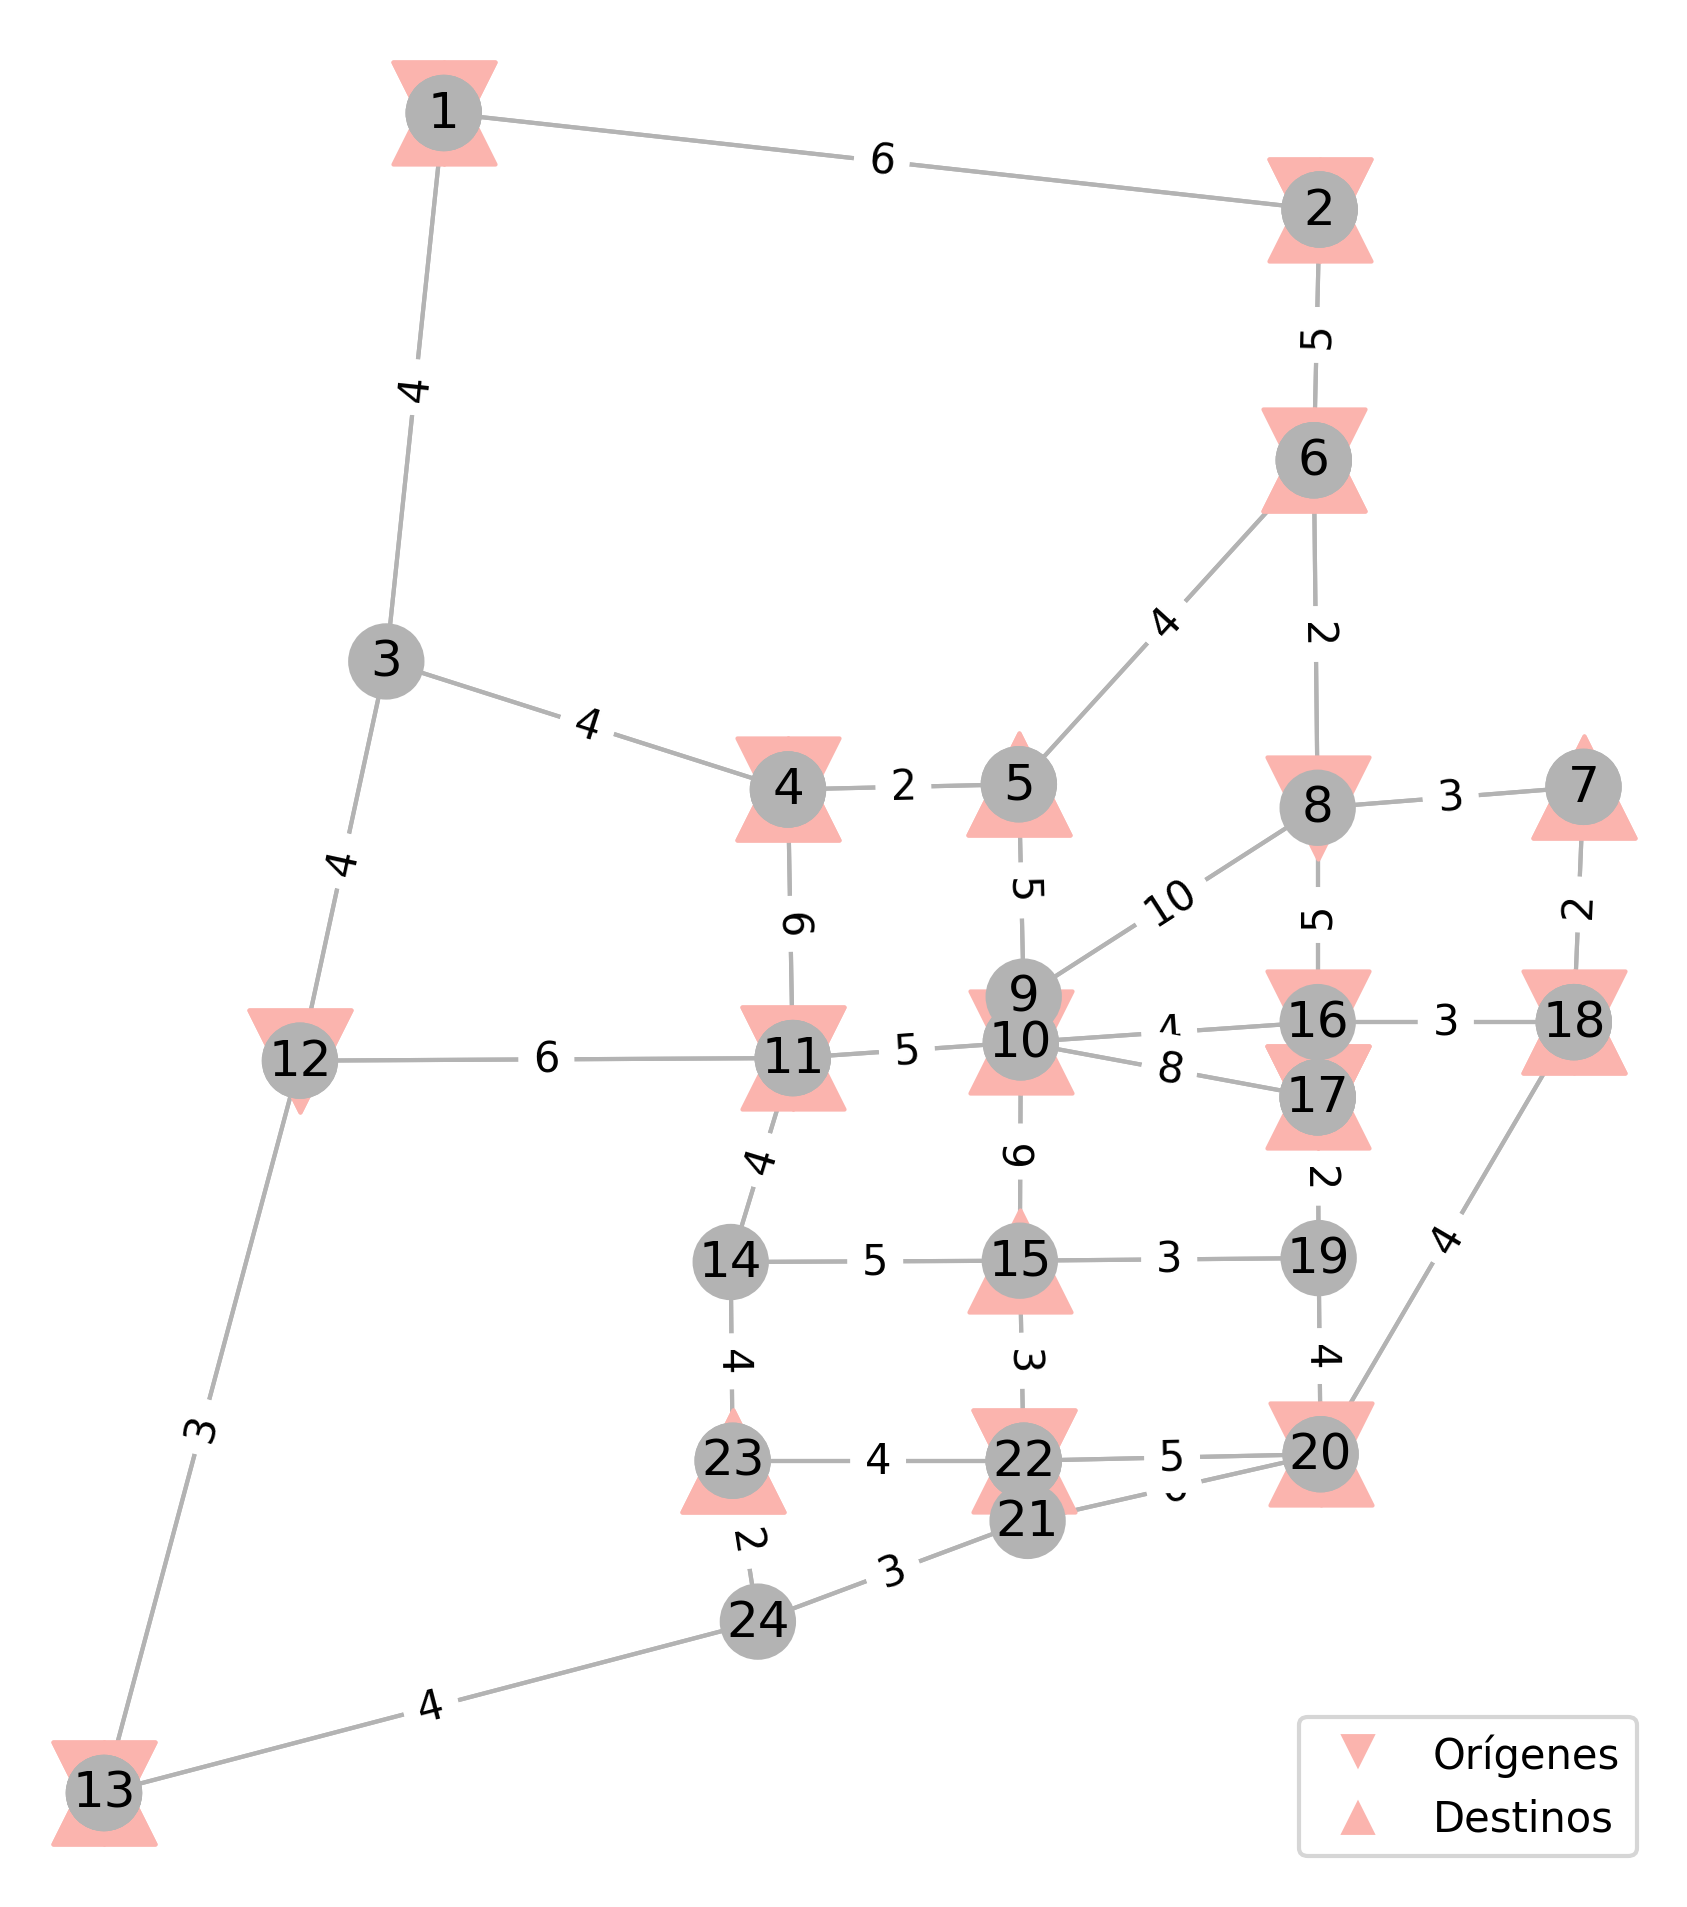
\includegraphics[width=8cm]{../resources/sioux_falls_odpairs.png}
\caption{Representación de la red de la instancia de Sioux-Falls.}
\label{fig:siouxfallsapendix}
\end{figure}

\begin{table}[h!]
\centering
\begin{tabular}{ccc}
  \toprule
    Arco & Costo \\
  \midrule
    (1, 2) & 6 \\
    (1, 3) & 4 \\
    (2, 1) & 6 \\
    (2, 6) & 5 \\
    (3, 1) & 4 \\
    (3, 4) & 4 \\
    (3, 12) & 4 \\
    (4, 3) & 4 \\
    (4, 5) & 2 \\
    (4, 11) & 6 \\
    (5, 4) & 2 \\
    (5, 6) & 4 \\
    (5, 9) & 5 \\
    (6, 2) & 5 \\
    (6, 5) & 4 \\
    (6, 8) & 2 \\
    (7, 8) & 3 \\
    (7, 18) & 2 \\
    (8, 6) & 2 \\
    (8, 7) & 3 \\
    (8, 9) & 10 \\
    (8, 16) & 5 \\
    (9, 5) & 5 \\
    (9, 8) & 10 \\
    (9, 10) & 3 \\
    (10, 9) & 3 \\
  \bottomrule
\end{tabular}
\begin{tabular}{ccc}
  \toprule
    Arco & Costo \\
  \midrule
    (10, 11) & 5 \\
    (10, 15) & 6 \\
    (10, 16) & 4 \\
    (10, 17) & 8 \\
    (11, 4) & 6 \\
    (11, 10) & 5 \\
    (11, 12) & 6 \\
    (11, 14) & 4 \\
    (12, 3) & 4 \\
    (12, 11) & 6 \\
    (12, 13) & 3 \\
    (13, 12) & 3 \\
    (13, 24) & 4 \\
    (14, 11) & 4 \\
    (14, 15) & 5 \\
    (14, 23) & 4 \\
    (15, 10) & 6 \\
    (15, 14) & 5 \\
    (15, 19) & 3 \\
    (15, 22) & 3 \\
    (16, 8) & 5 \\
    (16, 10) & 4 \\
    (16, 17) & 2 \\
    (16, 18) & 3 \\
    (17, 10) & 8 \\
    (17, 16) & 2 \\
 \bottomrule
\end{tabular}
\begin{tabular}{ccc}
  \toprule
    Arco & Costo \\
  \midrule
    (17, 19) & 2 \\
    (18, 7) & 2 \\
    (18, 16) & 3 \\
    (18, 20) & 4 \\
    (19, 15) & 3 \\
    (19, 17) & 2 \\
    (19, 20) & 4 \\
    (20, 18) & 4 \\
    (20, 19) & 4 \\
    (20, 21) & 6 \\
    (20, 22) & 5 \\
    (21, 20) & 6 \\
    (21, 22) & 2 \\
    (21, 24) & 3 \\
    (22, 15) & 3 \\
    (22, 20) & 5 \\
    (22, 21) & 2 \\
    (22, 23) & 4 \\
    (23, 14) & 4 \\
    (23, 22) & 4 \\
    (23, 24) & 2 \\
    (24, 13) & 4 \\
    (24, 21) & 3 \\
    (24, 23) & 2 \\
     & \\
     & \\
  \bottomrule
\end{tabular}
\caption{Costos de usuario de la tecnología base y de construcción de la tecnología 1 por arco de la red. Dado que utilizamos el largo del arco estos costos coinciden con dicho valor.}\label{table:siouxfallsgraphdata}
\end{table}

\begin{table}[h!]
\centering
\begin{tabular}{ccc}
  \toprule
    Origen & Destino & Demanda \\
  \midrule
    1 & 7 & 34 \\
    1 & 23 & 3 \\
    2 & 13 & 6 \\
    2 & 17 & 4 \\
    4 & 11 & 9 \\
    6 & 1 & 14 \\
    8 & 15 & 10 \\
    10 & 22 & 13 \\
    11 & 5 & 20 \\
    11 & 13 & 1 \\
    12 & 2 & 6 \\
    12 & 10 & 27 \\
    13 & 4 & 5 \\
    13 & 6 & 12 \\
    16 & 18 & 10 \\
    17 & 5 & 9 \\
    17 & 20 & 13 \\
    17 & 23 & 14 \\
    18 & 6 & 16 \\
    20 & 7 & 11 \\
    22 & 4 & 15 \\
    22 & 18 & 6 \\
  \bottomrule
\end{tabular}
\caption{Pares origen-destino utilizados para la red de Sioux-Falls junto a su valor de demanda.}\label{table:siouxfallsdemanddata}
\end{table}

  % Seguir copiando la linea de arriba para agregar más apéndices.

\end{document}
